\documentclass[12pt]{report}
\usepackage[utf8]{inputenc}
\usepackage[T1]{fontenc}
\usepackage[style=english]{csquotes}
\usepackage[english, spanish, catalan]{babel}
\usepackage{graphicx}
\usepackage{geometry}
\PassOptionsToPackage{hyphens}{url}\usepackage{hyperref}
\usepackage{titlesec}
\usepackage{lipsum}
\usepackage{fancyhdr}
\usepackage{amsmath}
\usepackage{amssymb}
\usepackage{tikz-cd}
\usepackage{subcaption}
\usepackage{stmaryrd}
\usepackage{url}
\usepackage{tikz}
\usetikzlibrary{shapes,
                tikzmark}
\tikzset{every tikzmarknode/.style={%
        draw=red, semithick, inner sep=2pt}
        }
\usepackage{forest}
\usetikzlibrary{fit,positioning}

\tikzset{
  red arrow/.style={
    midway,red,sloped,fill, minimum height=3cm, single arrow, single arrow head extend=.5cm, single arrow head indent=.25cm,xscale=0.3,yscale=0.15,
    allow upside down
  },
  black arrow/.style 2 args={-stealth, shorten >=#1, shorten <=#2},
  black arrow/.default={1mm}{1mm},
  tree box/.style={draw, rounded corners, inner sep=0.5em},
  node box/.style={white, draw=black, text=black, rectangle, rounded corners},
}
% Example definitions.
% --------------------

% Specific definitions
\def\Xtr{\mathbf{X}_{\text{tr}}}
\def\Ztr{\mathbf{Z}_{\text{tr}}}

% Packages
\usepackage{bm}
\usepackage{amssymb}
\usepackage{algorithmic}
\usepackage{algorithm}
\usepackage{url}
\usepackage{multirow}

% Functions
\def\trace{\operatorname{Tr}}
\def\dE{\mathbb E}
\def\KL{\mathbf{KL}}

% Number Sets
\def\real{{\mathbb R}}
\def\integer{{\mathbb Z}}
\def\natural{{\mathbb N}}

% Text
\def\p{{\mathrm{p}}}
\def\q{{\mathrm{q}}}
\def\rd{{\mathrm{d}}}

\def\F{{\mathrm{F}}}
\def\G{{\mathrm{G}}}
\def\H{{\mathrm{H}}}
\def\T{{\mathrm{T}}}

\def\KL{{\mbox{KL}}}
\def\TV{{\mbox{TV}}}

\def\tr{{\text{tr}}}

% Cal
\def\cC{{\mathcal C}}
\def\cH{{\mathcal H}}
\def\cL{{\mathcal L}}
\def\cN{{\mathcal N}}
\def\cX{{\mathcal X}}

% Bold Symbols and numbers
\def\bzero{{\mathbf 0}}
\def\bone{{\mathbf 1}}

% Greek letters
\def\balpha{{\boldsymbol{\alpha}}}
\def\bbeta{{\boldsymbol{\beta}}}
\def\bgamma{{\boldsymbol{\gamma}}}
\def\bdelta{{\boldsymbol{\delta}}}
\def\bepsilon{{\boldsymbol{\epsilon}}}
\def\bheta{{\boldsymbol{\eta}}}
\def\btheta{{\boldsymbol{\theta}}}
\def\biota{{\boldsymbol{\iota}}}
\def\bkappa{{\boldsymbol{\kappa}}}
\def\blambda{{\boldsymbol{\lambda}}}
\def\bmu{{\boldsymbol{\mu}}}
\def\bnu{{\boldsymbol{\nu}}}
\def\bxi{{\boldsymbol{\xi}}}
\def\bpi{{\boldsymbol{\pi}}}
\def\brho{{\boldsymbol{\rho}}}
\def\bsigma{{\boldsymbol{\sigma}}}
\def\btau{{\boldsymbol{\tau}}}
\def\bups{{\boldsymbol{\upsilon}}}
\def\bphi{{\boldsymbol{\phi}}}
\def\bchi{{\boldsymbol{\chi}}}
\def\bpsi{{\boldsymbol{\psi}}}
\def\bomega{{\boldsymbol{\omega}}}

\def\bAlpha{{\boldsymbol{\Alpha}}}
\def\bBeta{{\boldsymbol{\Beta}}}
\def\bGamma{{\boldsymbol{\Gamma}}}
\def\bDelta{{\boldsymbol{\Delta}}}
\def\bEpsilon{{\boldsymbol{\Epsilon}}}
\def\bHeta{{\boldsymbol{\Eta}}}
\def\bTheta{{\boldsymbol{\Theta}}}
\def\bIota{{\boldsymbol{\Iota}}}
\def\bKappa{{\boldsymbol{\Kappa}}}
\def\bLambda{{\boldsymbol{\Lambda}}}
\def\bMu{{\boldsymbol{\Mu}}}
\def\bNu{{\boldsymbol{\Nu}}}
\def\bXi{{\boldsymbol{\Xi}}}
\def\bPi{{\boldsymbol{\Pi}}}
\def\bRho{{\boldsymbol{\Rho}}}
\def\bSigma{{\boldsymbol{\Sigma}}}
\def\bTau{{\boldsymbol{\Tau}}}
\def\bUps{{\boldsymbol{\Upsilon}}}
\def\bPhi{{\boldsymbol{\Phi}}}
\def\bChi{{\boldsymbol{\Chi}}}
\def\bPsi{{\boldsymbol{\Psi}}}
\def\bOmega{{\boldsymbol{\Omega}}}

% Bold
\def\ba{{\mathbf a}}
\def\bb{{\mathbf b}}
\def\bc{{\mathbf c}}
\def\bd{{\mathbf d}}
\def\be{{\mathbf e}}
\def\bff{{\mathbf f}}
\def\bg{{\mathbf g}}
\def\bh{{\mathbf h}}
\def\bi{{\mathbf i}}
\def\bj{{\mathbf j}}
\def\bk{{\mathbf k}}
\def\bl{{\mathbf l}}
\def\bm{{\mathbf m}}
\def\bn{{\mathbf n}}
\def\bo{{\mathbf o}}
\def\bp{{\mathbf p}}
\def\bq{{\mathbf q}}
\def\br{{\mathbf r}}
\def\bs{{\mathbf s}}
\def\bt{{\mathbf t}}
\def\bu{{\mathbf u}}
\def\bv{{\mathbf v}}
\def\bw{{\mathbf w}}
\def\bx{{\mathbf x}}
\def\by{{\mathbf y}}
\def\bz{{\mathbf z}}

\def\bA{{\mathbf A}}
\def\bB{{\mathbf B}}
\def\bC{{\mathbf C}}
\def\bD{{\mathbf D}}
\def\bE{{\mathbf E}}
\def\bF{{\mathbf F}}
\def\bG{{\mathbf G}}
\def\bH{{\mathbf H}}
\def\bI{{\mathbf I}}
\def\bJ{{\mathbf J}}
\def\bK{{\mathbf K}}
\def\bL{{\mathbf L}}
\def\bM{{\mathbf M}}
\def\bN{{\mathbf N}}
\def\bO{{\mathbf O}}
\def\bP{{\mathbf P}}
\def\bQ{{\mathbf Q}}
\def\bR{{\mathbf R}}
\def\bS{{\mathbf S}}
\def\bT{{\mathbf T}}
\def\bU{{\mathbf U}}
\def\bV{{\mathbf V}}
\def\bW{{\mathbf W}}
\def\bX{{\mathbf X}}
\def\bY{{\mathbf Y}}
\def\bZ{{\mathbf Z}}

% Commands
%--------------------
\newcommand{\mean}[1]{\mathrm{<}#1\mathrm{>}}
\newcommand{\R}{\mathbb{R}}


%% Bibliography
\usepackage[backend=biber,style=numeric]{biblatex}
\DefineBibliographyStrings{english}{
  bibliography = {References},
}
\addbibresource{references.bib}

%% Cover, abstract and page style
%% Set up the geometry and hyperref packages
\geometry{
  a4paper,
  total={170mm,257mm},
  left=20mm,
  top=20mm,
}

\hypersetup{
    colorlinks=true,
    linkcolor=black,
    filecolor=magenta,
    urlcolor=cyan,
}

%% Define the cover page
\newcommand{\createcover}{
  \begin{titlepage}
    \centering
    
\includegraphics[width=0.3\textwidth]{logos/logo_FIB.png}\hspace{0.1cm}
    
\includegraphics[width=0.3\textwidth]{logos/logo_ETSETB.png}\hspace{0.1cm}
    
\includegraphics[width=0.25\textwidth]{logos/logo_FME.png}\\[1cm]
    
    {\large\bfseries BACHELOR'S DEGREE IN MATHEMATICS \\[0.3cm]  BACHELOR'S DEGREE IN DATA SCIENCE AND ENGINEERING}\\[1cm]
    
    {\huge\bfseries Automated detection of tumoural cells with graph neural networks}\\[1cm]

    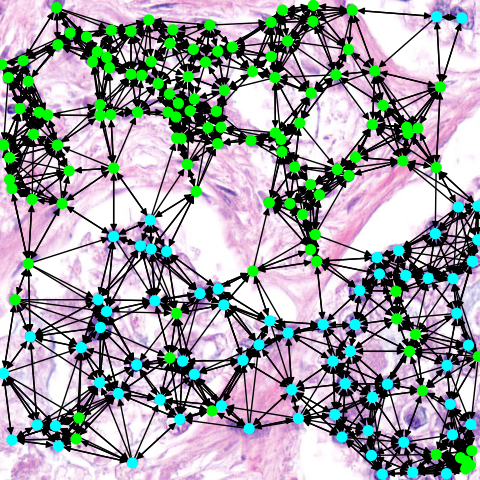
\includegraphics[width=0.7\textwidth]{imgs/graph_overlay.png}\\[2cm]
    
    {\large\itshape Author: Jose Pérez Cano}\\
    {\large\itshape Supervisor: Philippe Salembier Clairon}\\
    {\large\itshape Co-director: Ferran Marqués Acosta}\\[0.5cm]
    
    {\large June 2023}\\
    \vfill
    
\includegraphics[width=0.3\textwidth]{logos/logo_CFIS.jpg}
  \end{titlepage}
}

%% Define the abstract page
\newcommand{\createabstract}[4]{
\selectlanguage{#1}
\begin{abstract}
    \noindent #2 % Abstract text.
    \noindent \\
    \noindent #3 % Keywords.
    \noindent \\
    \noindent #4 % AMS codes
\end{abstract}
\selectlanguage{english}
}

%% Set up the headers and footers
\pagestyle{fancy} % Line on top of sections
\fancyhf{}
\renewcommand{\chaptermark}[1]{\markboth{#1}{}} 
\renewcommand{\sectionmark}[1]{\markright{\thesection\ #1}}
\fancyhead[L]{Jose Pérez Cano}
\fancyhead[R]{\leftmark}
\fancyfoot[C]{\thepage}
\fancypagestyle{plain}{
  \fancyhead{}
  \renewcommand{\headrulewidth}{0pt}
}

%% Customize the chapter and section formatting
\titleformat{\chapter}[display]
  {\normalfont\huge\bfseries}{\chaptertitlename\ \thechapter}{20pt}{\Huge}
\titlespacing*{\chapter}{0pt}{-30pt}{40pt}

%% Assemble the document
\begin{document}

\setlength{\headheight}{14.49998pt}
\addtolength{\topmargin}{-2.49998pt}

\createcover
\pagenumbering{roman}
\createabstract{english}{The detection of tumoural cells from whole slide images is an essential task in medical diagnosis and research. In this thesis, we propose and analyse a novel approach that combines computer vision-based models with graph neural networks to improve the accuracy of automated tumoural cell detection. Our proposal leverages the inherent structure and relationships between cells in the tissue. Experimental results on our own curated dataset shows that several different metrics improve by up to $15\%$ compared to just using the computer vision approach. It has been proved to work with H\&E stained lung tissue and HER2 stained breast tissue. We believe that our proposed method has the potential to improve the accuracy of automated tumoural cell detection, which can lead to accelerated diagnosis and research in the field by reducing the worload of hystopathologists.}{\textbf{Keywords:} Histology, Lung, Breast, Graph Neural Networks, Convolutional Neural Networks, Calibration.}{\textbf{AMS Codes:} 92C50, 92C55, 92C37, 68T10, 68T45, 68R10}
\clearpage
\createabstract{spanish}{La detección de células tumorales en imágenes de portaobjeto completo juega un papel esencial en el diagnóstico médico y es un elemento fundamental de la investigación sobre el cáncer. En esta tesis proponemos y analizamos un enfoque novedoso que combina modelos de visión por ordenador con redes neuronales en grafos para mejorar la precisión de la detección automatizada de células tumorales. Nuestra propuesta aprovecha la estructura inherente y las relaciones entre las células del tejido. Los resultados experimentales obtenidos sobre nuestra propia base de datos muestran que varias métricas mejoran hasta en un 15\% en comparación con solo usar el enfoque de visión. Se ha demostrado que funciona con tejido pulmonar teñido con H\&E y tejido mamario teñido con HER2. Creemos que nuestro método tiene el potencial de mejorar la precisión de los métodos automáticos de detección de células tumorales, lo que puede llevar a acelerar los diagnósticos y la investigación en este ámbito al reducir la carga de trabajo de los histopatólogos.}{\textbf{Palabras clave:} Histología, Pulmón, Mama, Redes Neuronales en Grafos, Redes Neuronales Convolucionales, Calibración.}{\textbf{Códigos AMS:} 92C50, 92C55, 92C37, 68T10, 68T45, 68R10}
\clearpage
\createabstract{catalan}{La detecció de cèl·lules tumorals en imatges de seccions completes és una tasca essencial en el diagnòstic mèdic i la investigació. En aquesta tesi, proposem i analitzem un enfocament innovador que combina models basats en visió amb xarxes neuronals en grafs per millorar la precisió de la detecció automatitzada de cèl·lules tumorals. La nostra proposta aprofita l'estructura inherent i les relacions entre cèl·lules en el teixit. Els resultats experimentals en el nostre propi conjunt de dades curat mostrin que diversos indicadors milloren fins a un 15\% en comparació amb només usar l'enfocament de visió. S'ha demostrat que funciona amb teixit pulmonar tenyit amb H\&E i teixit mamari tenyit amb HER2. Creiem que el nostre mètode proposat té el potencial de millorar la precisió de la detecció automatitzada de cèl·lules tumorals, el que pot portar a uns diagnòstics més ràpids i una investigació accelerada en el camp degut a la reducció en la càrrega de treball dels histopatòlegs.}{\textbf{Paraulas clau:} Histologia, Pulmó, Mama, Xarxes Neuronals en Grafs, Xarxes Neuronals Convolucionals, Calibració.}{\textbf{Codis AMS:} 92C50, 92C55, 92C37, 68T10, 68T45, 68R10}
\tableofcontents
\clearpage
\pagenumbering{arabic}

\chapter{Introduction}
\section{When technology meets histology}

This project was born due to the necessity of alleviating physicians and researchers workload in the field of digital pathology. On a typical day, our experts have to go through a wide variety of tissue images in order to detect some anomaly or disease. Depending on the task at hand they sometimes need to estimate the proportion of tumoural cells with respect to healthy ones. How wonderful would it be if a machine could perform that task for them. That is the purpose of this thesis, to automatically estimate the percentage of tumoural cells with respect to non-tumoural ones and facilitate the physician's job.

Analysing human tissue is a challenging task. The first part of the process consists of extracting the tissue from the part of the body that is relevant to the patient's condition. If the patient is alive the extraction is typically done using a needle. Otherwise, if the organ is already removed then a cube of tissue can be sliced. Then, simply watching those slices through a microscope is not going to be enough. Cells are very small and its interior is difficult to observe even when looking through the lenses of a microscope. For that reason tissue is stained prior to observing it. There are different kind of staining, some of them highlight the cell nuclei, others the membrane and other stainings react with specific kind of cells. Another factor to take into account is the cost of the dye. Some of them make the task at hand easier but are too expensive to do for every patient. A trade-off is usually found where the more expensive one is used only when the cheaper is not enough for confidently diagnosing.

In the past, the surgically extracted slices were typically watched through the lenses of a microscope \cite{Chen2011}, what is termed as optical microscopy. With the development of new technologies, the field has become more and more digitalised \cite{Kumar2020}, now being called digital pathology. The resulting digital images that originate from watching through the microscope the tissue are called Whole Slide Images (WSI). Between when a biopsy procedure is made and when the specialist watches it, there is now a period of time required to digitalise it. In other words, at the morning one specialist carries out the removal of the tissue. Afterwards, technicians digitalise the image in the afternoon. It is in the next morning the physician watches the result. Taking advantage of that interval between when the image is digitised and when the doctor watches it, other computational methods can be applied prior to the experts receiving the images. This will enhance the physician user experience while working without the need for them to wait for the algorithm to give the result at real time because it is already precomputed. Having a preliminary diagnosis can help reduce the workload and make the histologist more productive.

\section{Why graphs?}

This whole thesis was initially thought to be about lung tissue. Starting from a WSI we are interested in detecting which cells are tumoural and which cells are healthy. The purpose of the application is to rapidly detect tissue slices that contain a high amount of tumoural DNA so that it can be later on processed and analysed. Finding such WSI requires the histologist to look at several of them and deciding which one to choose. So we want to provide a ranking of images from more likely of having a high percentage of tumour to less likely. This way, on average, the physician would require to look at less images per patient, making it possible to analyse more patients' WSI in the same time. So, where does graphs come into play?

In a previous thesis, the same problem was tackled using a computer vision-only approach \cite{upcommons353765}. Initially, I was asked to improve on that method. After several months working on the problem I began to notice the principal flaw (which is also the principal feature) of convolutional neural networks: an inductive bias towards locality \cite{DBLP:journals/corr/CohenS16a}. That means deep neural networks classify cells based on their immediate morphological properties. However, having met with pathologist Irene Sansano Valero, which is an expert histologist in the field of lung tumour, made it clear that cells were considered being tumoural or not depending on their surroundings. Visually identical cells may be classified differently if their neighbourhood is different. Here, I am always referring to lung tissue, we will later on analyse if this still holds true for other tissues. It was made clear then that a different approach was needed. Another kind of inductive bias was required, a relational inductive bias. One that classified cells based on their relationships with nearby cells and not only on their individual properties. This is the exact kind of inductive bias graph neural networks provide \cite{DBLP:journals/corr/abs-2104-13478}. 

This is how the idea came into existence. The exact details of how the graph is constructed and which networks are employed are later discussed. But the key idea is that if relations between cells are considered important when classifying them, using graphs in some way may lead to better results. We expect this hypothesis to be specially true for lung tissue and, in fact, we come across high evidence that it is so. The question then is, is it true for other tissues? The answer is it depends. Apart from the lung dataset we repeat all the experiments for other three datasets obtaining mixed results. Sometimes it is a good fit, sometimes it is not and sometimes it works better but not because it is a graph but because it is a stacking classifier. The exact meaning of these words and which experiments are made to prove it will be later discussed.
\chapter{Problem Formulation and State Of The Art}

\section{Definition}

In order to estimate the percentage of tumoural cells we decided to solve other problem. Instead of just predicting a number from a WSI, which would make the problem a logistic regression problem, we decided to segment and classify every cell to later count them and compute the percentage. There are two reasons why we chose to do so. The first one is because it makes models more interpretable, and the second one is because it makes the problem easier to solve.

Developing more on that first reason, we work in the medical field. Here, having a model that is statistically better than, say, a student is not enough to consider it really better than the student. The student can explain itself on why it made that diagnosis and so it provides more insight on how and why it makes mistakes. A seemingly black box model that simply outputs a number (the percentage of tumoural cells) gives no insight whatsoever of how and when you may expect it to fail. This is very dangerous in a medical setting. If we were at a factory classifying packages, we don't care so much about that. We can recover lost packages later on while still benefiting from the efficiency of using a automated process. However, we cannot recover dead patients. That makes interpretability a must. If our model predicts cells we can see which cells are causing more trouble. This helps know which data is needed to used for retraining the model and fixing those mistakes in the future. In the end, we want a model that can learn from its mistakes, looking at individual cell predictions makes it easier to recognise patterns in the mistakes it is doing and so it makes it easier to incrementally improve the model from its errors.

The second reason is that the regression problem is harder to solve. It may seem to be the other way around but it is not. Having worked with machine learning problems for years, my experience is that a regression problem where images are the input is almost never a good idea. Reframing the problem to solve something apparently harder in between has brought me better results in the past. Nonetheless, let's describe mathematically each problem in order to analyse each of them and come to an intuition of why it is a bad idea.

First, let's denote by $\mathcal{X}$ and $\mathcal{Y}$ the input and output space of the problem. We expect to find a function $f : \mathcal{X} \to \mathcal{Y}$ that effectively predicts the correct percentage given the WSI. Any WSI is no more than a collection of pixels, for that reason they can be viewed as very high dimensional vectors $\mathcal{X} = \mathbb{R}^N$, with $N > 10^{9}$ \cite{DICOM}. Similarly, the percentage is just a number between 0 and 1, so $\mathcal{Y} = [0,1]$.

Now, the logistic regression approach consists of finding such function from a family of parametric models $\mathcal{F}_\theta = \{ f_\theta | f_\theta : \mathcal{X} \to \mathcal{Y} \}$ while the segmentation approach tries to find $f$ differently. It first divides the WSI into patches. Then, each patch is processed independently to obtain pixel-wise predictions which are then used to compute the percentage. So, the family of parametric models now in consideration is $\mathcal{G}_\theta = \{ g_\theta | g_\theta : \mathcal{X}_s \to \mathcal{X}_s,\ \mathcal{X}_s \subset \mathcal{X} \}$ where $\mathcal{X}_s$ represents the space of images of 1024 by 1024 pixels, meaning $\text{dim}(\mathcal{X}_s) \approx 3.1 \cdot 10^6$. Given any segmentation model $g_\theta$ we construct its regression counterpart $f_\theta$ as described in the following commutative diagram. 

\[ \begin{tikzcd}
\mathcal{X} \arrow{r}{f_\theta} \arrow[swap]{d}{s} & \mathcal{Y} \\%
\mathcal{X}_s^P \arrow{r}{\tilde{g}_\theta}& \mathcal{X}_s^P \arrow{u}{c}
\end{tikzcd}
\]

Where we have extended $g_\theta$ to several patches by applying it independently to all of them.

\begin{align}
\begin{split}
\tilde{g}_\theta : \mathcal{X}_s^P& \to \mathcal{X}_s^P\\
(x_1, ..., x_P)& \mapsto (g_\theta(x_1), ..., g_\theta(x_P))
\end{split}
\end{align}

And the $s$ and $c$ functions refer to the split and count operations. Given a WSI it is split into several patches, for each patch, every cell is segmented and then all the tumoural and healthy cells are counted.

Without making any further assumptions about the families of functions we can derive some important insights about the advantages and disadvantages of each approach. First of all, it is clear that in the first approach the models have access to a wider context. Considering independent patches limits the ability to take into account global information. For instance, in lung tissue there is a structure called the cilium. It is a filamentous structure that appears near bronchioles. Its own existence is reason enough for considering the nearby cells as healthy. An example of such structure is depicted on \autoref{fig:lung-cilium}. The presence of cilium in the middle of a WSI cannot be taken into account when classifying the border of the tissue. But this disadvantage is not such a big deal. In a 1024 by 1024 image there is room enough for all the cells affected by the cilium, so limiting to such patches is enough. There is also another type of cell that interacts with their surrounding, the erythrocyte, also called red blood cell. All the cells glued to it are considered healthy. But that only applies to very close cells to it, so by using patches you will have no problem with this type of interactions. On the other hand, if we look at the dimensionality of input and output spaces we see a clear difference between the two approaches. For $\mathcal{F}_\theta$ the input space has a huge dimensionality while the output is uni-dimensional. In contrast, for $\mathcal{G}_\theta$ the input and output space both have the same dimensionality which is several orders of magnitude smaller than the dimensionality of $\mathcal{X}$. This makes the first approach quite prone to the curse of dimensionality \cite{AnalyticsVidhya}\footnote{Notice that this is not true for other regression problems, NeRFs \cite{mildenhall2020nerf} need to increase the dimensionality of the input to work properly.}. Even worse, we have just one number per each WSI. Even a simple regression problem needs more than 30 samples to have a reasonable amount of uncertainty. Having such amount of WSI is a very difficult task.

One may also think that the regression problem can be split into patches too. That is, solving the problem for individual patches and then averaging the percentages. This way the difference in dimensionality of the input and output spaces is lower. Moreover, the data scarcity problem is solved. But it is not so easy. In my experience, even with 224 by 224 images, regression is quite unfeasible if done in a naive way. On the other hand, for the individual percentages of each patch to be enough we will need to label all the patches of a WSI. Otherwise the sampling may not be uniform enough since WSI are very different from one part of the image to another, in other words, they are highly non-stationary. Labelling all the patches of one WSI could mean labelling thousands of images, which is unfeasible.

All in all, we chose this way because we believed it was going to give better results and because the doctors preferred that solution over the other for its interpretability.


\section{Data labelling}\label{sec:data}

As stated in the previous section we have access to few WSI but each WSI contains a lot of information. One can extract hundreds of patches from surgical biopsies made by thoracotomy, and even in needle biopsies it is possible to obtain more than two hundred patches. However, those images are of no use without their corresponding labels. To illustrate what we are referring to, look at \autoref{fig:labels} below.

\begin{figure}[ht]
  \centering
  \begin{subfigure}[b]{0.45\textwidth}
    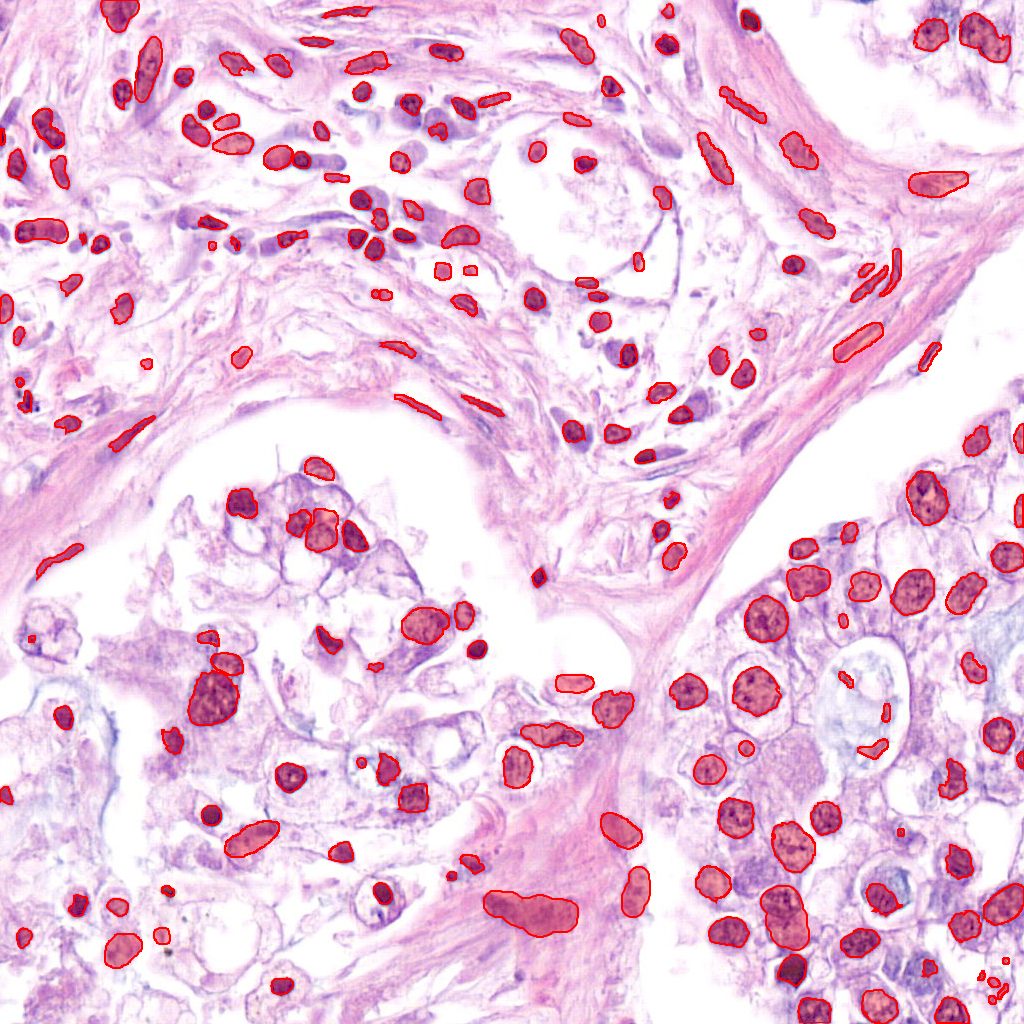
\includegraphics[width=\textwidth]{imgs/seg.png}
    \caption{Segmentation}
    \label{fig:seg}
  \end{subfigure}
  \hfill
  \begin{subfigure}[b]{0.45\textwidth}
    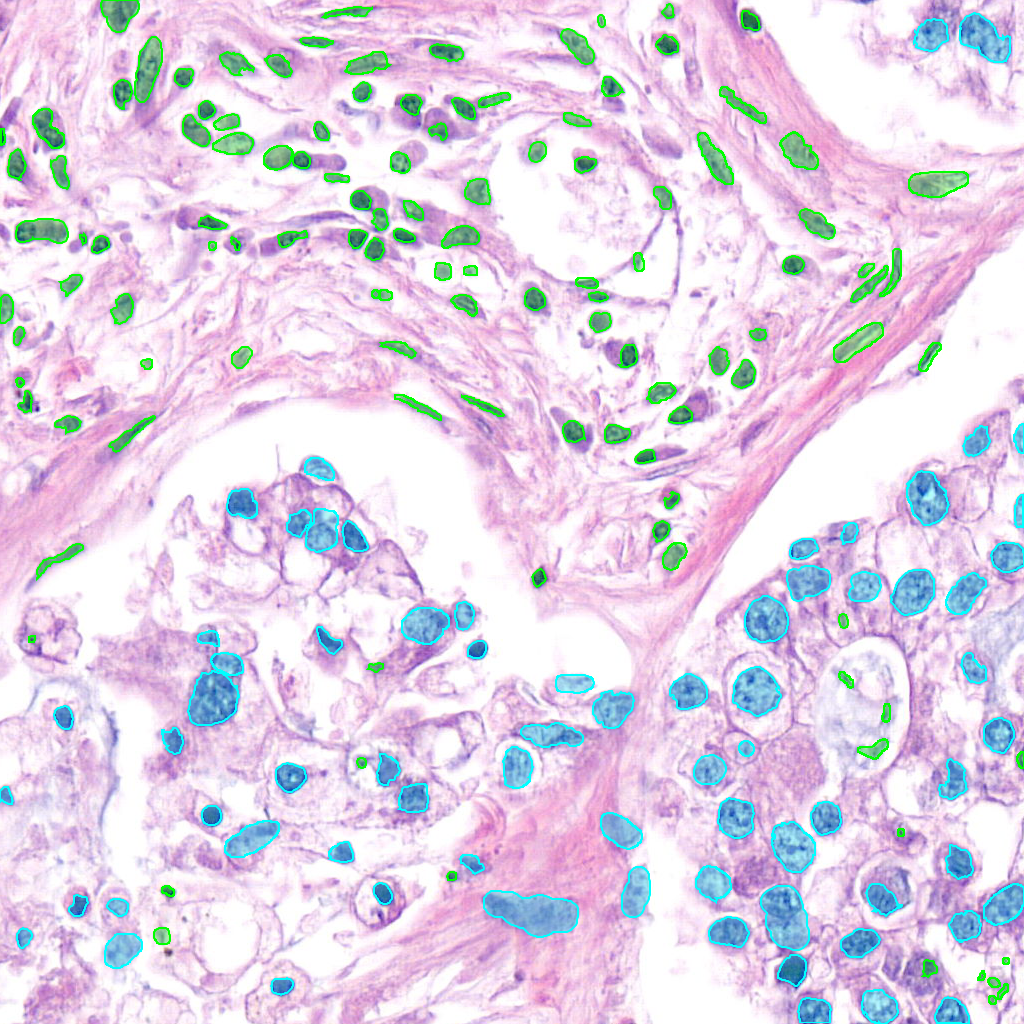
\includegraphics[width=\textwidth]{imgs/overlay.png}
    \caption{Classification}
    \label{fig:class}
  \end{subfigure}
  \caption{Visualisation of the kind of labels that are needed. For each cell it is required to have its contour, as seen in the left, together with their corresponding class as seen in the right. Blue means tumoural and green non-tumoural.}
  \label{fig:labels}
\end{figure}

The ground truth (GT) used to train the models needs to be handcrafted, which is a tedious process. To alleviate the amount of work required, an iterative procedure was designed. In a first step made by David Anglada and Feliu Formosa, the max-tree \cite{maxtree} was used to create rough segmentations of 24 patches that were later reviewed and improved by the students. Those initial labels were used to train Hovernet \cite{hovernet}, explained in detail in \autoref{sec:vision}. Using that newly trained model, 20 more images were annotated and reviewed by me. Then, Hovernet was trained again using those 44 images and used to infer the GT of 41 more patches. Only after carefully correcting all the 85 slices, would the pathologist Irene Sansano Valero start reviewing the dataset. The whole process took around 100 hours of human labour, around 20 hours of GPU computation and 10 hours of expert human labour.

\section{Computer vision algorithms}\label{sec:vision}

In this section I will provide a brief survey about the state of the art in segmentations problems and a detailed explanation of Hovernet \cite{hovernet} which is the model used in the first phase of our method.

The first deep learning attempt at biomedical segmentation was made by Olaf Ronneberger et al. \cite{unet}. They proposed an encoder-decoder architecture as shown in \autoref{fig:unet}.

\begin{figure}[ht]
    \centering
    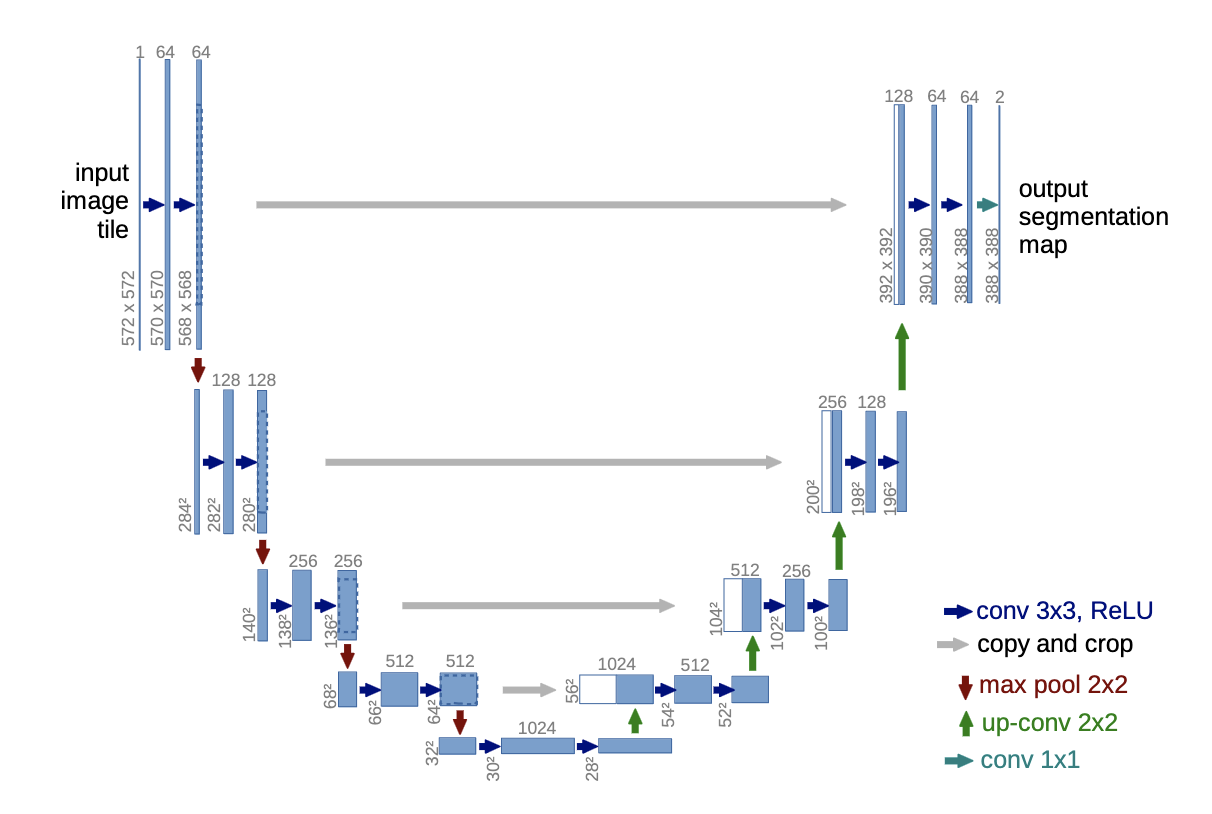
\includegraphics[width=\textwidth]{imgs/unet.png}
    \caption{Original U-net architecture. It was composed by convolutional layers, pooling layers and residual connections.}
    \label{fig:unet}
\end{figure}

That architecture was improved recently with the development of transformers \cite{transformer}. In 2021 Jieneng Chen et al. invented TransUNet \cite{transunet} and later on in 2022 Jeya Maria Jose Valanarasu et al. created UNeXt \cite{unext}. I will not dive into the specifics of those architectures but rather comment on their limitations and why we couldn't use them. The key limitation is their sample efficiency. Even though transformers are more sample efficient in reinforcement learning than previous deep learning methods \cite{micheli2023transformers}, they still require a fair amount of data. In Jeya Maria Jose Valanarasu et al. \cite{unext} they used two datasets of 2594 and 647 images respectively. That is at least an order of magnitude more than what we could obtain. The other option, TransUNet \cite{transunet}, was tried in a dataset with 3779 computer tomography (CT) images, yet too much for us. Apart from that, the problem they tackled was organ segmentation, which is quite different from cell segmentation. In order to achieve better sample efficiency, a method with specific inductive biases is needed.

As explained in \autoref{sec:data}, the max-tree \cite{maxtree} can give good results at detecting cell contours while using no data at all. The algorithm used morphological properties of the cells to distinguish them from the background. That set a precedent, morphological algorithms could help us reduce the amount of data needed. Another important morphological algorithm is the watershed \cite{watershed}. It is known for creating accurate contours if the energy landscape is properly defined. Hovernet \cite{hovernet} combines both the U-net architecture with the watershed algorithm to produce cell segmentations and classify them. An overview is on \autoref{fig:hovpipe}.

\begin{figure}[ht]
    \centering
    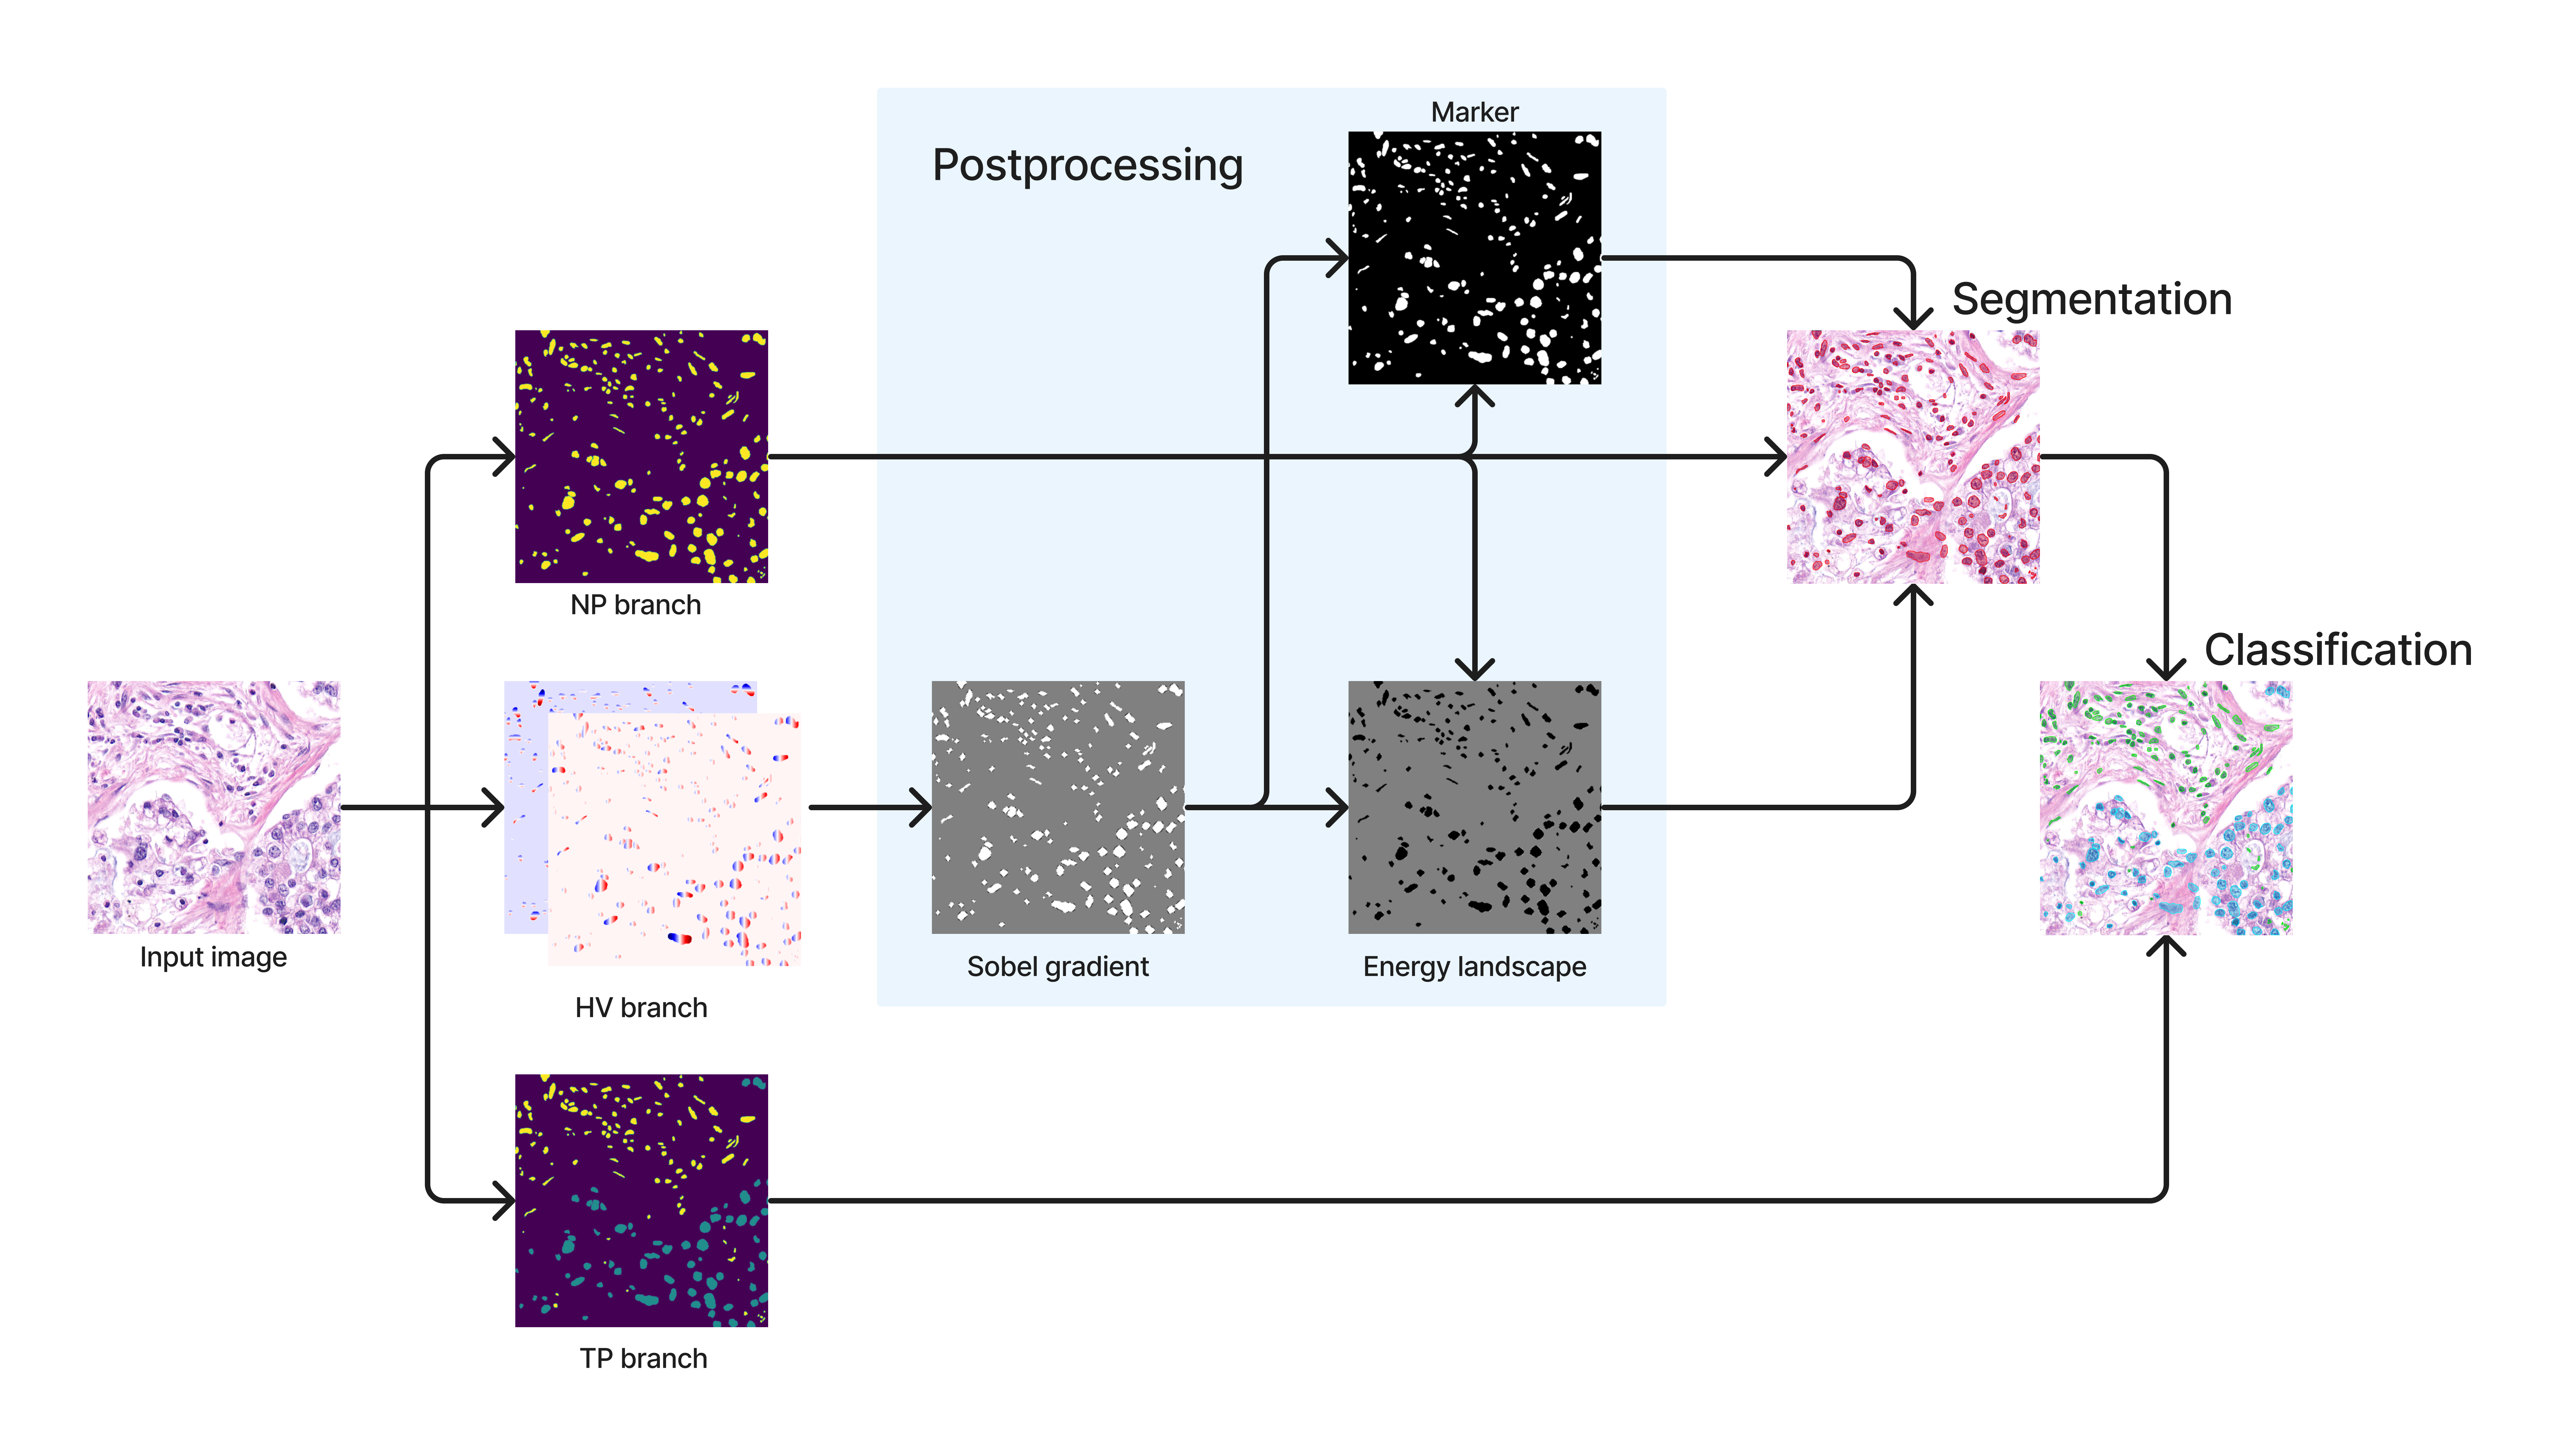
\includegraphics[width=\textwidth]{imgs/hovpipe.png}
    \caption{Overview of the Hovernet method. It has three branches that predict different maps derived from the GT. In a post-processing step all the maps are combined using the watershed algorithm with carefully designed energy landscapes and markers.}
    \label{fig:hovpipe}
\end{figure}

Hovernet employs the same encoder-decoder architecture as U-net but it combines three different decoders with only one shared encoder. Each of the three decoders is trained to infer a different property from the GT. The NP branch separates the cells from the background, ignoring their class. The HV branch predicts horizontal and vertical distances from each pixel to the nuclei of the nearest cell. And the TP branch predicts the GT as is. Everything is trained end-to-end under one single loss function, which is shown below

\begin{align}
    \mathcal{L} &= \lambda_{mse}^{HV}\mathcal{L}_{mse}^{HV} + \lambda_{msge}^{HV}\mathcal{L}_{msge}^{HV} + \lambda_{bce}^{NP}\mathcal{L}_{bce}^{NP} + \lambda_{dice}^{NP}\mathcal{L}_{dice}^{NP} + \lambda_{bce}^{TP}\mathcal{L}_{bce}^{TP} + \lambda_{dice}^{TP}\mathcal{L}_{dice}^{TP} \\
    &= \frac{\lambda_{mse}^{HV}}{B}\left( \sum_{i=0}^{B} \| H(x_i) - h_i \|_2^2 + \sum_{i=0}^{B} \| V(x_i) - v_i \|_2^2 \right) \\
    &+ \frac{\lambda_{msge}^{HV}}{B}\left( \sum_{i=0}^{B} \| \nabla H(x_i) - gh_i \|_2^2 + \sum_{i=0}^{B} \| \nabla V(x_i) - gv_i \|_2^2 \right) \\
    &+ \frac{\lambda_{bce}^{NP}}{B} \sum_{i=0}^B \sum_{j=0}^{D} (y_{i}^{NP})_j \log (NP(x_i)_j) \\
    &+ \frac{\lambda_{dice}^{NP}}{B} \sum_{i=0}^B \left(1 - \frac{\sum_{j=0}^D NP(x_i)_j (y_{i}^{NP})_j}{\sum_{j=0}^D (NP(x_i)_j)^2 + \sum_{j=0}^D ((y_{i}^{NP})_j)^2}\right)\\
    &+ \frac{\lambda_{bce}^{TP}}{B} \sum_{i=0}^B \sum_{j=0}^{D} (y_{i}^{TP})_j \log (TP(x_i)_j) \\
    &+ \frac{\lambda_{dice}^{TP}}{B} \sum_{i=0}^B \left(1 - \frac{\sum_{j=0}^D TP(x_i)_j (y_{i}^{TP})_j}{\sum_{j=0}^D (TP(x_i)_j)^2 + \sum_{j=0}^D ((y_{i}^{TP})_j)^2}\right)
\end{align}

\noindent where all the $\lambda$ are hyperparameters, the letter $y$ denotes GT in any form, $h$ and $v$ are horizontal and vertical GT maps, $gh$ and $gv$ are the gradients of horizontal and vertical maps, $D$ is the number of pixels in any image, $B$ is the batch size, $\| \cdot \|_2^2$ is the $L_2$ norm, $H(\cdot)$ and $V(\cdot)$ are the outputs of the HV branch, $NP(\cdot)$ the output of the NP branch and $TP(\cdot)$ the output of the TP branch.

After the model is trained, it can be used for inference in addition with a post-processing phase which consists of the watershed algorithm. This particular watershed requires an energy landscape which defines the space where the flooding is made and a marker that contains the starting points to start the flooding. Both are defined below

\begin{align}
    E &= (1 - \mathcal{S}_m(\bX)) \odot NP(\bX) \\
    M &= \text{ReLU}(NP(\bX) - \mathcal{S}_m(\bX))
\end{align}

\noindent being $E$ the energy and $M$ the marker. In those equations $\bX$ refers to the input image, ReLU is the rectified linear unit \cite{relu}, $\odot$ is the element-wise multiplication, also referred to as Hadamard product, and $\mathcal{S}_m(\bX)$ is the thresholded gradient of the HV branch as expressed here

\begin{equation}
    \mathcal{S}_m(\bX) = \max(S_x * H(\bX), S_y * V(\bX))
\end{equation}

\noindent where $S_x$ and $S_y$ are Sobel filters \cite{sobel} and $*$ is the convolution operation. The whole process can be visualized in \autoref{fig:hovpipe}. 

%% Postprocessing step

\section{Graph neural networks}\label{sec:gnn}

Having described the state of the art for computer vision, let's introduce the state of the art of graph neural networks as well. There are more than 50 different possible architectures \cite{graph_survey} and more than 300.000 possible configurations \cite{you2021design}. However I will focus mainly on two of the most popular architectures: graph convolution and graph attention. Both can be used for node classification which is what we are interested about since we are going to treat cells as nodes. More on that description in \autoref{sec:descr}.

\subsection{Graph convolution}\label{sec:gcn}

This architecture was proposed by Thomas N. Kipf et al. \cite{graphconv} in 2016 and has been cited almost ten thousands times as of this date. The main idea is to adapt the notion of convolution from images to graphs. An illustration of the concept can be seen in \autoref{fig:conv_comp}.

\begin{figure}[ht]
    \centering
    \begin{subfigure}[b]{0.4\textwidth}
        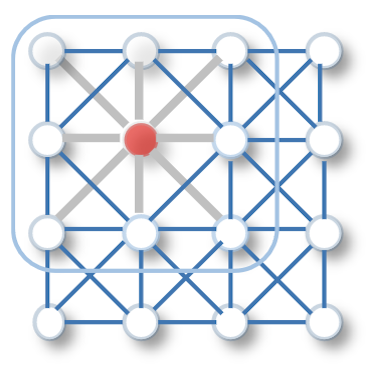
\includegraphics[width=\textwidth]{imgs/conv.png}
        \caption{2D Convolution where each pixel can be considered a node connected to all its adjacent pixels. This operation returns the weighted average of adjacent pixels for each node.}
    \end{subfigure}
    \hfill
    \begin{subfigure}[b]{0.4\textwidth}
        
\includegraphics[width=\textwidth]{imgs/graph conv.png}
        \caption{Graph Convolution where the weighted average is taken with respect to adjacent nodes. There is no notion of pixels and each node has no absolute spatial coordinates.}
    \end{subfigure}
    \caption{Visualisation of 2D Convolution vs Graph Convolution taken from \cite{graph_survey}.}
    \label{fig:conv_comp}
\end{figure}

Mathematically, the graph convolution operation as expressed in \cite{graphconv} can be defined as shown below

\begin{equation}
    \bh_j^{(l+1)} = \sigma \left(\bb^{(l)} + \sum_{k \in \mathcal{N}_j} \frac{1}{c_{jk}} \bW^{(l)}\bh_k^{(l)}\right)
\end{equation}

\noindent where $\bb^{(l)}\in \R^d, \bW^{(l)} \in \R^{d\times d}$ are the bias and weights of the layer, $\mathcal{N}_j$ is the set of neighbours of node $j$, $c_{jk} = \sqrt{|\mathcal{N}_j|\cdot |\mathcal{N}_k|}$ is a normalisation factor and $\sigma$ is an activation function. The vectors $\bh_k^{(l)}$ are the hidden embeddings of the network for each layer, being $\bh_k^{(0)}$ an initial vector containing any relevant information about the node. That information can be the area of the cell, the average colour, or even a prior distribution for the class label. In the last layer, the weight matrix is of dimensions $C \times d$, where $C$ is the number of classes or $1$ if $C=2$ and the activation function is either the sigmoid for a binary problem or the softmax \cite{softmax} for a multi-class problem.

\subsection{Graph attention}

As an improvement over simply doing the average, one year after the publication of the graph convolution, Petar Veličković et al. \cite{graphatt} proposed the idea of including the attention mechanism \cite{attention} to compute a weighted average instead. This idea, which has been cited over eight thousands times, is visualised in \autoref{fig:gat}.

\begin{figure}[ht]
    \centering
    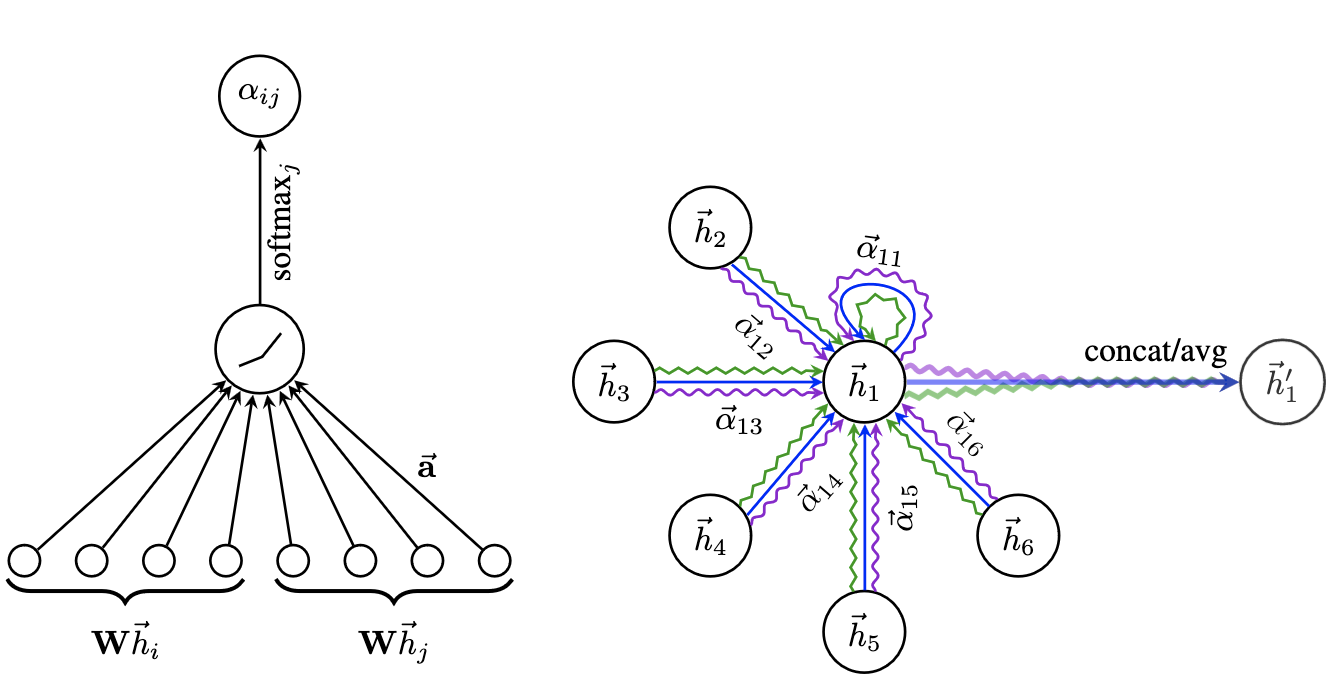
\includegraphics[width=\textwidth]{imgs/gat.png}
    \caption{On the left is the overview of the computation of the attention weights. For each adjacent node an attention weight is computed based on the similarity of their embeddings. On the right there is a visualisation about multi-head attention, which consists of concatenating the result of several attention mechanisms. The figures are taken from the original article \cite{graphatt}.}
    \label{fig:gat}
\end{figure}

More formally, the computation can be described as follows

\begin{equation}
    \bh_j^{(l+1)} = \sigma \left(\sum_{k \in \mathcal{N}_j} \alpha_{jk} \bW^{(l)}\bh_k^{(l)}\right)
\end{equation}

\noindent where $\bW^{l}\in \R^{d\times d}$ are the layer weights and $\alpha_{jk} \in \R$ are the attention weights which are defined by the following formula

\begin{equation}
    \alpha_{jk} = \frac{\exp(\text{LeakyReLU}(\ba \cdot [\bW \bh_j||\bW \bh_k]))}{\sum_{r\in \mathcal{N}_j} \exp(\text{LeakyReLU}(\ba \cdot [\bW \bh_j||\bW \bh_r]))}
\end{equation}

\noindent being $\ba \in \R^{2d'}, \bW \in \R^{d'\times d}$ two learnable projection matrices, LeakyReLU is the leaky rectified linear unit \cite{leakyrelu} and $||$ the concatenation operation. Inspired by the multi-head attention mechanism proposed in \cite{transformer}, the previous attention mechanism can be extended to $H$ heads

\begin{equation}
    \bh_j^{(l+1)} = \bigparallel_{h=1}^H \sigma \left(\sum_{k \in \mathcal{N}_j} \alpha_{jkh} \bW^{(l)}_h\bh_k^{(l)}\right)
\end{equation}

\noindent where now $\bW^{(l)}_h \in \R^{d \times Hd}$, the attention weights are different for each head and sum up to one in each head $\sum_{k\in\mathcal{N}_j}\alpha_{jkh}=1,\ \forall h$ and in the final layer heads are averaged instead of concatenated as explained in \cite{graphatt}.
\chapter{Problem Solving}

Having described the problem at hand as well as relevant deep learning methods it is time to join it all into one single method. In this chapter we will cover a detailed explanation of the method proposed, the metrics that will be used to compare across architectures and hyperparameters, the experiments carried out to show its usefulness and the results obtained.

\section{Method description}\label{sec:descr}

I have described how the cell classification problem was tackled with the help of convolutional neural networks. I have also explained two algorithms used for node classification. It is time to merge both fields. For that, we need to describe the cell classification problem as a node classification problem. As mentioned in \autoref{sec:gnn}, the nodes of our graph are going to be the individual cells. It is left to define the edges. We are going to consider two nodes (cells) to be related if they are sufficiently close. By sufficiently close it is meant that their euclidean distance is less than some previously defined amount. Apart from that, to have manageable graphs, the degree of each node is limited by only considering a small amount of nearby nodes as possible connections. This way we ensure the number of edges increases linearly with the number of nodes making our method more scalable. An example of such graph is on \autoref{fig:graph_def}. 

\begin{figure}[h]
    \centering
    \begin{subfigure}{0.3\textwidth}
      \centering
      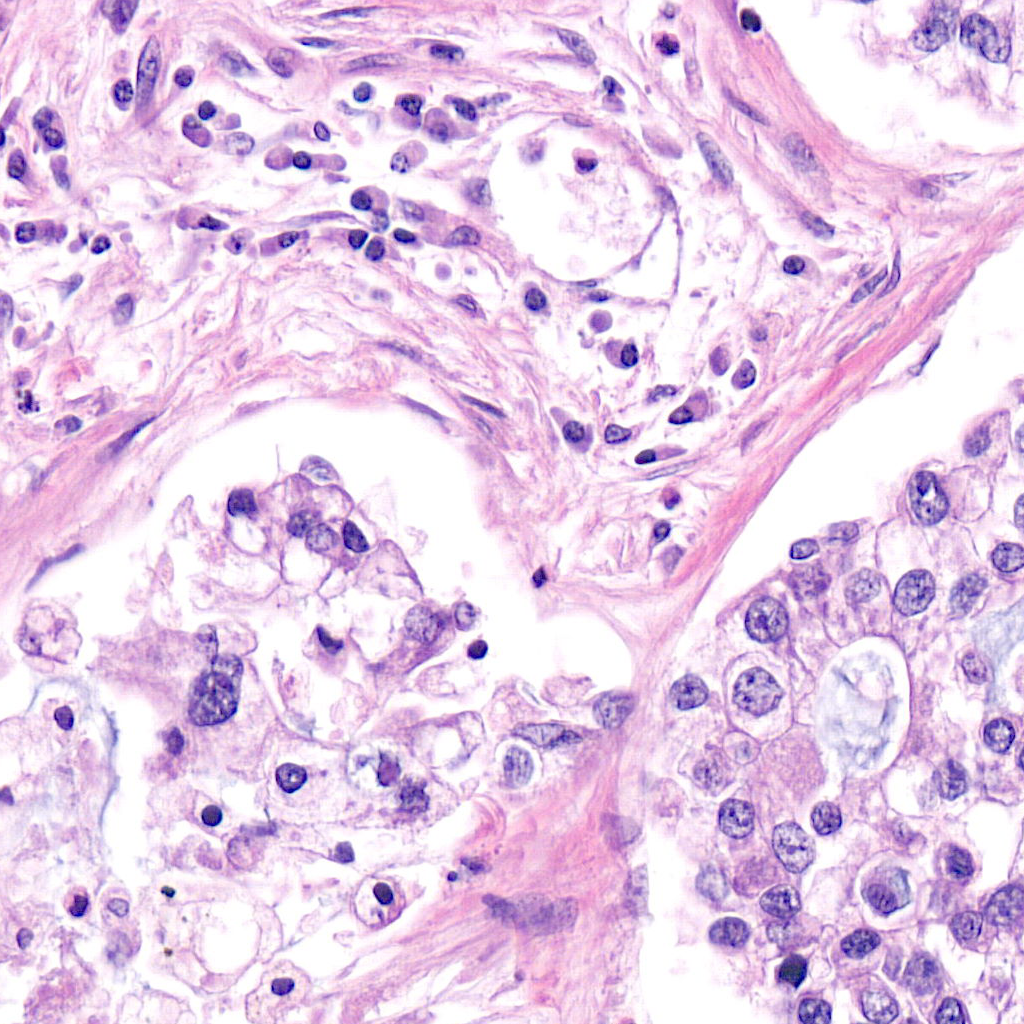
\includegraphics[width=\textwidth]{imgs/img_ex.png}
    \end{subfigure}
    \begin{subfigure}{0.3\textwidth}
      \centering
      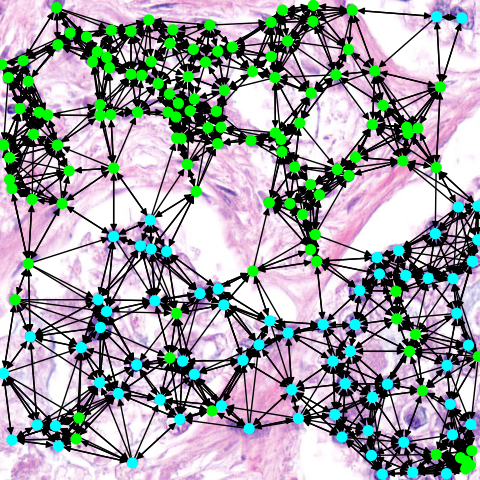
\includegraphics[width=\textwidth]{imgs/graph_overlay.png}
    \end{subfigure}
    \begin{subfigure}{0.3\textwidth}
      \centering
      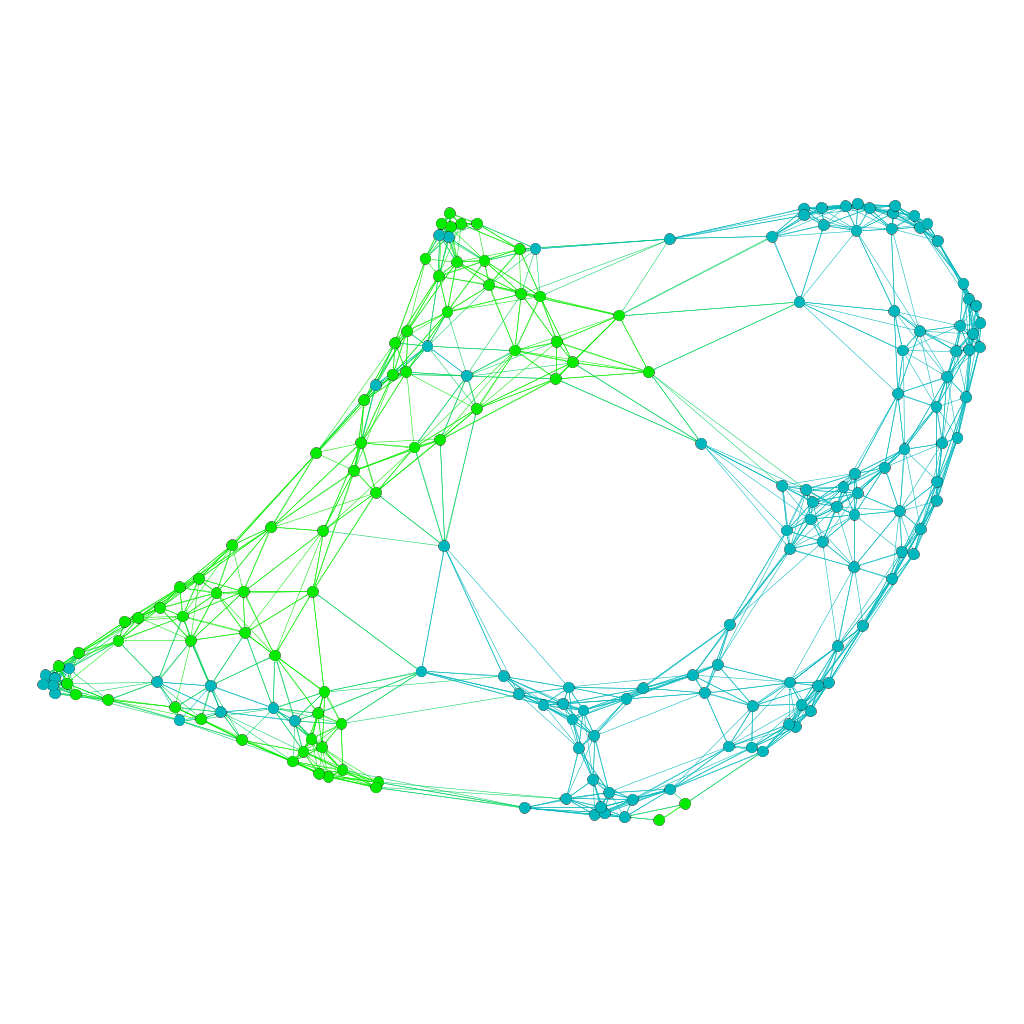
\includegraphics[width=\textwidth]{imgs/graph_class.png}
    \end{subfigure}
    \caption{Example of an image and its associated graph. At the middle we have the nodes located at their corresponding centroids. However, a graph is an abstraction, so it may also be viewed as in the right image, since it only encodes relationships, not absolute positions. The visualization of the graph was made using Gephi \cite{gephi}.}
    \label{fig:graph_def}
\end{figure}

Given nodes and edges we can still give more information to the graph neural network. In \autoref{sec:gcn} we showed that the network can be given an initial set of features $\bh_k^{(0)}$. Those features can be anything that gives information about the cell. We decided to use the following set of descriptive features:

\begin{itemize}
    \item The area and perimeter of the cell measured in pixels. Those values should give information about the shape of the cell.
    \item The standard deviation of the values of the pixels in gray format. This magnitude is supposed to bring insights about the luminosity of the cell.
    \item The histogram of the red, green and blue colour channels. We expect it to summarise the information about the colour of the cell.
    \item A prior distribution of the class. It is computed using the output of Hovernet. Each class probability is inferred as the number of pixels of that class predicted by Hovernet divided by the total number of pixels of the cell.
\end{itemize}

\noindent Later on, in \autoref{sec:exp} an experiment is made to discover how relevant the selected features are.

\section{Evaluation metrics}\label{sec:metrics}

This section is going to provide a review of the most common metrics for any classification problem, either binary of multiclass. 

\subsection{Confusion Matrix}

Prior to defining any metric we have to define the concept of confusion matrix. Most of the metrics described can be expressed in terms of it. The confusion matrix is a way of measuring how precise is any method. For a binary classification problem one has positive (1) and negative (0) classes. If the model correctly predicts the positive or negative class it is called true positive and true negative. Then, if the model incorrectly predicts positive it is called false positive and if it infers negative wrongly it is denoted by false negative. Confusion matrices are typically expressed as shown below.

\begin{table}[ht]
\centering
\caption{Binary confusion matrix.}
\begin{tabular}{c c c|c|}
& & \multicolumn{2}{c}{\textbf{Predicted}} \\ \cline{3-4}
& & \multicolumn{1}{|c|}{Positive} & Negative \\ \cline{2-4}
\multirow{2}{*}{\textbf{Actual}} & \multicolumn{1}{|c|}{Positive} & $TP$ & $FP$ \\ \cline{2-4}
                     & \multicolumn{1}{|c|}{Negative} & $FN$ & $TN$ \\ \cline{2-4}
\end{tabular}
\label{table:confusion_matrix}
\end{table}

For more than two classes sometimes an adaptation is made. Instead of adding more rows and columns the matrix is built considering one class against all the others. In that case several confusion matrices are needed. Of course, one can also create a bigger confusion matrix as follows

\begin{table}[ht]
\centering
\caption{Multi-class confusion matrix. Here the terms true positive, negative and false positive, negative lack any meaning unless you consider one class against the others.}
\label{table:confusion_matrix2}
\begin{tabular}{c c c|c|c|c|c|}
& & \multicolumn{5}{c}{\textbf{Predicted}} \\ \cline{3-7}
& & \multicolumn{1}{|c|}{Class 1} & Class 2 & Class 3 & Class 4 & Class 5 \\ \cline{2-7}
\multirow{5}{*}{\textbf{Actual}} & \multicolumn{1}{|c|}{Class 1} & & & & & \\ \cline{2-7}
                     & \multicolumn{1}{|c|}{Class 2} & & & & & \\ \cline{2-7}
                     & \multicolumn{1}{|c|}{Class 3} & & & & & \\ \cline{2-7}
                     & \multicolumn{1}{|c|}{Class 4} & & & & & \\ \cline{2-7}
                     & \multicolumn{1}{|c|}{Class 5} & & & & & \\ \cline{2-7}
\end{tabular}
\end{table}

\subsection{Accuracy}\label{sec:acc}

The first metric we will be defining is the most intuitive one. It is basically the percentage of correct predictions. Using the terminology from \autoref{table:confusion_matrix} it can be expressed as 
\begin{equation}
    \frac{TP + TN}{TP + FP + TN + FN}
\end{equation}

The main disadvantage of the accuracy comes when dealing with imbalanced datasets. By predicting the class that appears the most a high accuracy can be easily achieved in those cases.

The accuracy is a binary classification metric, later on in \autoref{sec:micro} an adaptation to multi-class problems is described.

\subsection{Precision}

The accuracy requires to know how many true negatives there are. But in some problems like object detection that is not always possible. Due to how labels are constructed in some cases it is impossible to know how many true negatives can be considered, although in the case of object detection the trend seems to be changing these days \cite{kirillov2023segment}. In those cases it makes sense to define the percentage of correct predictions only within the positive class. Mathematically, precision is defined as

\begin{equation}
    P = \frac{TP}{TP + FP}
\end{equation}

This metric, however, can be easily fooled. In an image with hundreds of cells, by only predicting one true tumoural cell you achieve a precision of $100\%$. But that is a useless value since you would be missing on most relevant cells.

\subsection{Recall}

As opposed to precision, recall focuses more on what relevant values are retrieved rather than them being correct. It is defined like this

\begin{equation}
    R = \frac{TP}{TP + FN}
\end{equation}

Again, this metric can also be fooled. By predicting everything as positive you achieve $100\%$. Since this metric ignores false positives you are left with a biased metric against the negative label.

\subsection{$F_1$ Score}\label{sec:f1}

In order to take the best from precision and recall, the F-measure was proposed in 1992 at the Proceedings of the 4th conference on Message understanding \cite{10.5555/1072064}. The F-measure is defined as the harmonic mean between precision and recall.

\begin{equation}
    \frac{2 \cdot P \cdot R}{P + R} = \frac{2 \cdot TP}{2 \cdot TP + FP + FN}
\end{equation}

Nowadays it is called $F_1$ score because that measure has been extended to what is called the $F_\beta$ score.

\begin{equation}
    F_\beta = \frac{(1+\beta^2) \cdot P \cdot R}{\beta^2 \cdot P + R} = \frac{(1+\beta^2) \cdot TP}{(1+\beta^2) \cdot TP + \beta^2 \cdot FP + FN}
\end{equation}

\noindent By taking $\beta=1$ the original F-measure is obtained. This metric achieves $100\%$ when all the relevant positive samples are retrieved and only the relevant samples, therefore it is not so easily fooled. Moreover, it is less prone to suffer from class imbalance as the accuracy does.

There are three ways of extending the $F_1$ score to a multi-class classification problem. All of them involve some kind of averaging the individual $F_1$ scores computed by considering one class against all the others. 

\subsection{Macro $F_1$ Score}

The first way of averaging individual $F_1$ scores is by simply taking the arithmetic mean. If we have $n$ classes, and we call $F_1^i$ the $F_1$ score of the class $i$ against the others, then the macro $F_1$ score is

\begin{equation}
    \frac{1}{n} \sum_{i=1}^n F_1^i
\end{equation}

The main drawback of only considering this metric is that classes can be imbalanced. In fact, for multi-class problems that is the rule rather than the exception. Giving equal weights to all of the classes harms the less represented labels.

\subsection{Weighted $F_1$ Score}

As a way of solving the main drawback of the macro $F_1$ score one can deal with the weighted $F_1$ score that averages individual scores based on their support, that is, based on the number of true instances by class. Let's call $n_i$ the number of true instances of class $i$, then the weighted $F_1$ score is

\begin{equation}
    \sum_{i=1}^n \frac{n_i \cdot F_1^i}{n_1 + \dots + n_n}
\end{equation}

\subsection{Micro $F_1$ Score}\label{sec:micro}

Another way of averaging the individual $F_1$ scores is by micro-averaging. When macro-averaging, true positives, false negatives and false positives are computed per-class prior to averaging all the scores computed as defined in \autoref{sec:f1}. Micro-averaging changes the order. True positives, false negatives and false positives are first aggregated among all the classes and then the micro $F_1$ score is computed using the formula in \autoref{sec:f1}. To illustrate the computation let's consider the matrix from \autoref{table:confusion_matrix2} and let's also fill it with false positives / negatives and true positives, giving the matrix in \autoref{table:confusion_matrix3}. Now, this terminology only makes sense when splitting by class. For that reason we will denote by $TP_i$ the true positives of class $i$, and $FP_i$, $FN_i$ the false positives and negatives of same class $i$. Notice that what is a false positive for one class can be a false negative for another.

\begin{table}[ht]
\centering
\caption{Multi-class confusion matrix. The values in the diagonal are all true positives when considering one class agains the others. Depending on which class you are considering, the values considered false positives and false negatives could be interchanged.}
\begin{tabular}{c c c|c|c|c|c|}
& & \multicolumn{5}{c}{\textbf{Predicted}} \\ \cline{3-7}
& & \multicolumn{1}{|c|}{Class 1} & Class 2 & Class 3 & Class 4 & Class 5 \\ \cline{2-7}
\multirow{5}{*}{\textbf{Actual}} 
 & \multicolumn{1}{|c|}{Class 1} & $TP_1$ & $FP_1$, $FN_2$ & $FP_1$, $FN_3$ & $FP_1$, $FN_4$ & $FP_1$, $FN_5$ \\ \cline{2-7}
 & \multicolumn{1}{|c|}{Class 2} & $FP_2$, $FN_1$ & $TP_2$ & $FP_2$, $FN_3$ & $FP_2$, $FN_4$ & $FP_2$, $FN_5$ \\ \cline{2-7}
 & \multicolumn{1}{|c|}{Class 3} & $FP_3$, $FN_1$ & $FP_3$, $FN_2$ & $TP_3$ & $FP_3$, $FN_4$ & $FP_3$, $FN_5$ \\ \cline{2-7}
 & \multicolumn{1}{|c|}{Class 4} & $FP_4$, $FN_1$ & $FP_4$, $FN_2$ & $FP_4$, $FN_3$ & $TP_4$ & $FP_4$, $FN_5$ \\ \cline{2-7}
 & \multicolumn{1}{|c|}{Class 5} & $FP_5$, $FN_1$ & $FP_5$, $FN_2$ & $FP_5$, $FN_3$ & $FP_5$, $FN_4$ & $TP_5$ \\ \cline{2-7}
\end{tabular}
\label{table:confusion_matrix3}
\end{table}

The micro-average is then the sum of the diagonal divided by the sum of all the entries in the matrix. It is quite similar to how the accuracy is computed. For that reason sometimes this metric is referred to as the accuracy in multi-class problems.

\newpage
\subsection{Dice's coefficient}

The Dice's coefficient can be viewed as a generalisation of the $F_1$ score. Given two sets $X$ and $Y$ the Dice's coefficient is defined as 

\begin{equation}
    \frac{2\cdot |X \cap Y|}{|X| + |Y|}
\end{equation}

If we consider $X$ as the set of relevant items and $Y$ as the set of retrieved elements, we obtain the $F_1$ score. To show that, let's see what are the sets of retrieved and relevant objects. The relevant items are the sum of true positives and false negatives. The retrieved ones are the sum of true positives and false positives. The intersection is clearly just the true positives, so $|X\cap Y| = TP$ and also $|X|+|Y|=2\cdot TP + FN + FP$. Substituting into the formula for the Dice's coefficient the formula for the $F_1$ score appears.

But the Dice's coefficient can be used for more than that. It can be used as a metric for image segmentation problems. By defining $X$ as the set of pixels that belongs to a class in the ground truth and $Y$ as the set of pixels of the same class but in the predictions, the Dice's coefficient can be used for evaluating the performance of a segmentation model. 

Furthermore, it is possible to extend that measure to a loss function. All the metrics presented so far require a thresholding function at the end. That function has a discontinuity at $0.5$ but worse than that, are completely flat in the rest of the $[0,1]$ interval, which means the gradient is zero. A null gradient stops any deep learning method from using them as loss functions. The adaptation of the Dice's coefficient to a loss was made by Milletari et al. \cite{milletari2016vnet}. The idea is to take advantage from the fact that pixel class probabilities range from 0 to 1. The Dice's coefficient can be seen as a boolean operation. Therefore, the Dice's loss is a function that when given just 0s and 1s is that same boolean operation, but is also defined in the rest of the $[0,1]$ interval and not just in the extremes. To be consistent with the original notation, let's call $p_i$ to the predicted probabilities and $g_i$ to the ground truth probabilities, where $i$ ranges from $1$ to $N$ being $N$ the total number of pixels. Thus, the Dice's loss is

\begin{equation}
    D = \frac{2 \sum_{i=1}^N p_i g_i}{\sum_{i=1}^N p_i^2 + \sum_{i=1}^N g_i^2}
\end{equation}

It is clear that when $p_i \in \{0,1\} \forall i$ and $g_i \in \{0,1\} \forall i$ the result is the same as the Dice's coefficient. But in this new version, the gradient can be computed with respect to any pixel with this formula.

\begin{equation}
    \frac{\partial D}{\partial p_j} = 2\cdot \frac{g_j\left(\sum_{i=1}^N p_i^2 + \sum_{i=1}^N g_i^2\right) - 2p_j \sum_{i=1}^N p_ig_i}{\left(\sum_{i=1}^N p_i^2 + \sum_{i=1}^N g_i^2 \right)^2}
\end{equation}

\subsection{ROC AUC}

Another metric that avoids thresholding the probabilities is the Receiver Operating Characteristic Area Under the Curve. It evaluates the ordering of the probabilities instead of the actual predictions. Before diving into the details of the ROC curve, we need to first define the false positive rate.

\begin{equation}
    FPR = \frac{FP}{FP + TN}
\end{equation}

False positives and true negatives depend on the threshold selected. Using $0.5$ gives some predictions while using $-1$ give everything as positive and using $2$ returns all negatives. By changing the threshold different FPR are obtained. Moreover, the Recall, also known as true positive rate (TPR), changes when using different thresholds too. There is a balance between both of them, similar to what happened with precision and recall. Both metrics can be fooled, but not at the same time. So by changing the threshold one can measure which metric is being fooled the most. The ROC curve plots the TPR in the y axis and the FPR in the x axis. An example is on \autoref{fig:auc}.

\begin{figure}[ht]
    \centering
    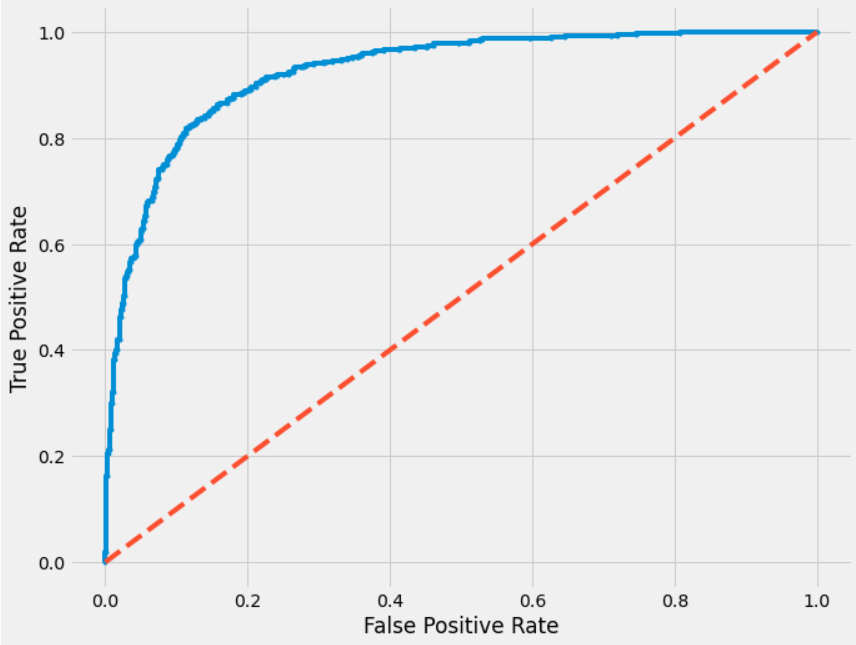
\includegraphics[width=\textwidth]{imgs/auc.png}
    \caption{Example of a ROC curve.}
    \label{fig:auc}
\end{figure}

This curve always starts in the $(0,0)$ and finishes in the $(1,1)$ corresponding to thresholds $2$ and $-1$ respectively (or any other threshold that returns all negatives and all positives). Given that, the ROC AUC is, as its name states, the area under that curve. A random classifier would yield the orange line in \autoref{fig:auc} that goes from $(0,0)$ to $(1,1)$, while a perfect classifier would go from $(0,0)$ to $(0,1)$ and then to $(1,1)$. Therefore, any classifier has an AUC roughly between $0.5$ and $1$. Notice that an AUC of $0$ corresponds to an adversarial classifier, which is a perfect classifier but changes negatives with positives.

\subsection{Calibration}

To finish this section, I'll cover a different way of evaluating classifiers. Normally, the effectiveness of a classifier is measured depending on how well it classifies samples. But that has its flaws too. It may be interesting to have a way of measuring the uncertainty of a prediction. If I am going to be diagnosed with cancer I want to know how likely that is wrong. Having a $51\%$ probability of dying is not the same as having a $99.9\%$ probability. None of the previous metrics evaluates the quality of the uncertainty provided by the probabilities. Deep learning methods oftentimes suffer from overconfidence \cite{wei2022mitigating, meronen2023fixing, melotti2022reducing}. Neural networks typically provide probabilities that are close to $1$ even when the available information is not enough to be so sure about that prediction. To analyse that phenomena, reliability diagrams were invented. An example is provided in \autoref{fig:rel}. On the x axis there is the predicted probability while in the y axis is an estimation of the real probability.

\begin{figure}[ht]
    \centering
    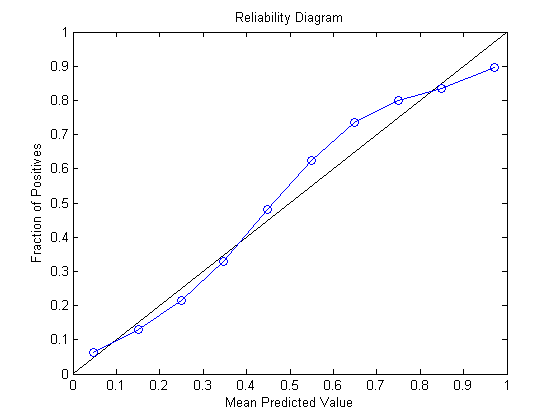
\includegraphics[width=\textwidth]{imgs/rel.png}
    \caption{Example of a reliability diagram.}
    \label{fig:rel}
\end{figure}

More specifically, predicted probability is quantised. The x axis represents the probability distribution of the model, but we only have a finite collection of samples, so that distribution is estimated using the histogram. This means that the points in \autoref{fig:rel} in fact represents a set of samples that are predicted with very similar probabilities. The magnitude in the y axis is how many of them really are positive. As an example, suppose we have 4 samples predicted with probabilities $0.74, 0.75, 0.75, 0.76$ and only three of them are real positives. The mean predicted probability of that group is $0.75$, and the real probability is also $0.75$ since 3 out of 4 are positives. This would give a point in the black line, a perfectly calibrated point. On the other hand, consider the following example. Four samples, 3 with probability 1 and 1 with probability 0. From the first three, one is negative and two are positive. The sample with probability 0 is negative. In this case, we have a point at $(0,0)$ and another at $(1,\frac{2}{3})$. This time, we have a less calibrated prediction. Nonetheless, in both examples we have an accuracy of $75\%$. This illustrates the fact that calibration is independent from how well you classify samples. An example of an uncalibrated model is on \autoref{fig:hov_rel}.

\begin{figure}[ht]
    \centering
    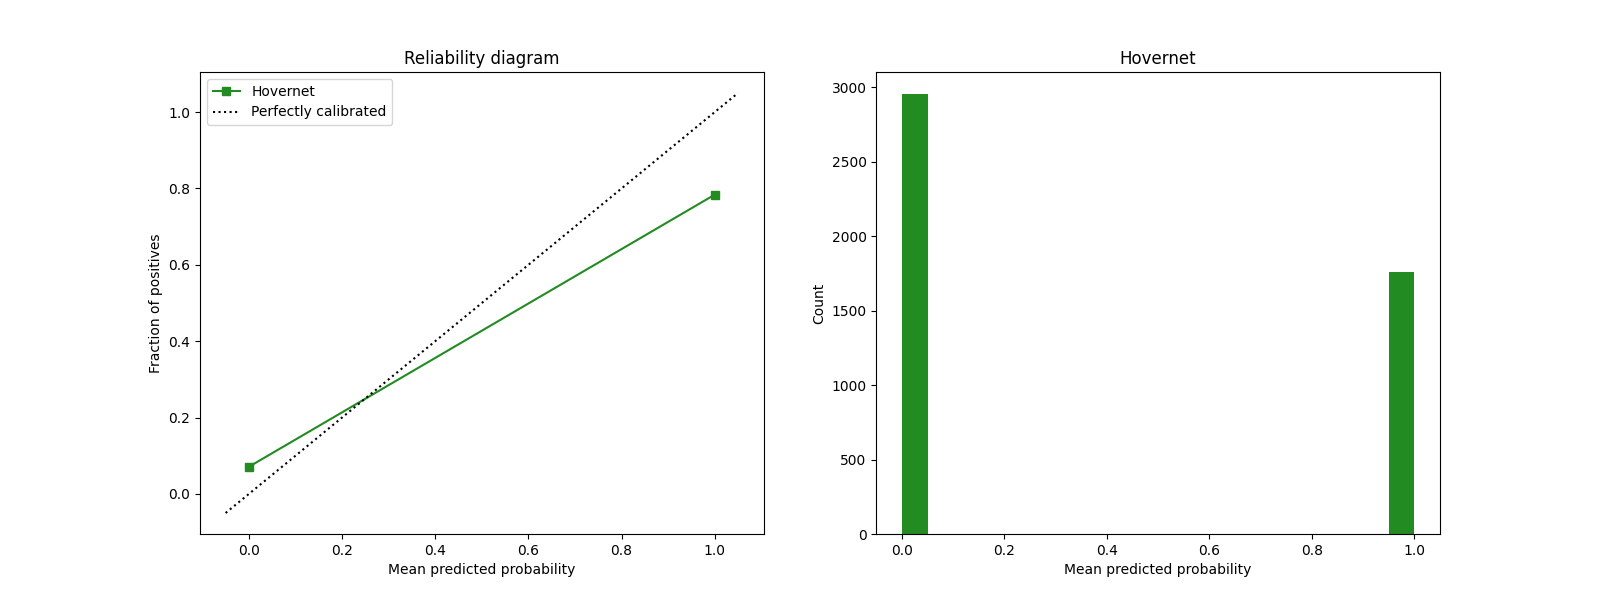
\includegraphics[width=\textwidth]{imgs/hov_rel_diag.png}
    \caption{Reliability diagram of Hovernet from one of our experiments. At the right is the histogram of the predicted probabilities, clearly not a uniform distribution.}
    \label{fig:hov_rel}
\end{figure}

Reliability diagrams can be converted into a metric in the same way the ROC was made a metric by using the area under it. Here, instead of the area under the curve, the area between the model curve and a perfectly calibrated curve is taken. Furthermore, since points in that diagram can represent sets of arbitrary size the area of each bin is weighted by the number of samples in it. Where now we are calling the points bins, since in fact, each point has a width that represents the range of probabilities it takes into account. A more appropriate visualisation is on \autoref{fig:rel2}. The metric derived is called Expected Calibration Error (ECE).

\begin{figure}[ht]
    \centering
    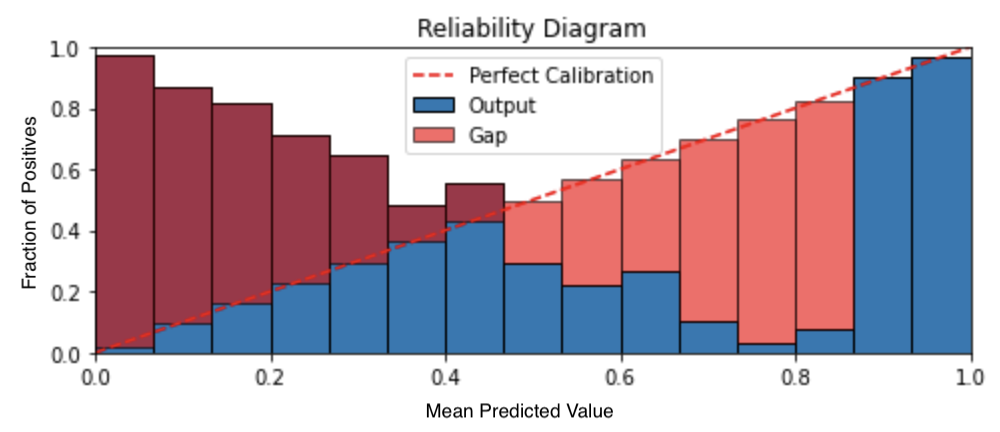
\includegraphics[width=\textwidth]{imgs/rel2.png}
    \caption{Another way of representing a reliability diagram.}
    \label{fig:rel2}
\end{figure}

\subsection{Extending metrics}

I have depicted a clear way of measuring uncertainty calibration in the previous section but it has at least one downside, it is only for binary problems. I'll devote this subsection to a way in which one can extend any binary metric to a multiclass metric. Suppose we have a metric called $M$.  Now, given a multiclass setup one can compute $M^k$, the same metric but considering the class $k$ against the others. By grouping all the other classes into one, the problem is now binary and so we can compute $M$. By averaging all the $M^k$ we get the extension of $M$. For instance, the macro $F_1$ score correspond to doing this to the $F_1$ score with equal weights to all classes. While the weighted $F_1$ score is the weighted average of the individual $F_1$ scores. However, the micro $F_1$ score, which is also called accuracy, does not correspond to the extension of the accuracy, although it is quite close. The extension of the accuracy is in fact $\frac{2}{N} \text{Micro} + \frac{N-2}{N}$ being $N$ the number of classes. The proof is straightforward. If we call $D$ the diagonal of the confusion matrix and $T$ the total sum then

\begin{align}
    Acc^k &= \frac{a_{kk} + \sum_{i,j \neq k} a_{ij}}{\sum_{i,j}a_{ij}} \\
    Acc_{extended} &= \frac{1}{N} \sum_{k} Acc^k = \frac{\sum_{k}a_{kk} + \sum_{k} \sum_{i,j\neq k} a_{ij}}{N \sum_{i,j}a_{ij}} \\
    &= \frac{2D + (N-2) T}{N T} = \frac{2}{N} \text{Micro} + \frac{N-2}{N}
\end{align}

where the intermediate step can be deduced by counting how many times does each term appears. The diagonal terms appear $N-1$ times while the rest of terms appear $N-2$ times, therefore $\sum_{k} \sum_{i,j\neq k} a_{ij} = D + (N-1)T$, concluding the proof. Surprisingly enough, the extension of the accuracy approaches 1 as the number of classes increases so it is quite a bad metric. In the experiments below, we will be using the extension of the ECE and call it just ECE for simplicity in the multiclass datasets.

\section{Experiments}\label{sec:exp}

Two experiments were carried out to show the usefulness of graph neural networks in the problem of cell detection and another two experiments were made to provide insights about the models involved. Results are in \autoref{sec:results}, this section is only to describe the experiments themselves. 


\subsection{GNN vs CNN}

The main experiment and the one that supports the principal thesis of this work compares convolutional neural networks with graph neural networks. In order to state that GNNs are actually useful they must outperform CNNs (Hovernet) in every metric defined in \autoref{sec:metrics}. But outperforming in just one dataset is not enough. For that reason the comparison will be made using all the datasets from the original Hovernet article \cite{hovernet, gamper2020pannuke, 8880654}, and using several internal datasets of the DigiPatics project \cite{DigiPatics2022}. More concretely, the methods will be evaluated in the HER2 stained breast dataset and the H\&E stained lung dataset. For the multi-class problems, multi-class metrics will be taken into account and for binary problems, binary metrics.

\subsection{GNN vs XGBoost}

Outperforming CNNs may not be due to the graph structure. It is possible that the extracted features are sufficient to improve CNN results. It may be that the edges do not contain any useful information. To account for that, GNN must be compared with node-only methods. In this case we selected XGBoost \cite{xgboost} for comparison since it has been in the leaderboard of several Kaggle competitions\footnote{\url{https://dataaspirant.com/xgboost-algorithm/}}. By comparing node-only methods with GNNs we can know if the value of GNNs reside on the extracted features or on the graph structure itself.

\subsection{Scaling CNNs}

The original Hovernet article restricted their images to having 270x270 pixels. That is a very narrow view of the cells. It seems intuitive that increasing the receptive field of the model increases its performance too. But science does not understand intuition, only facts. So an experiment needs to be carried out in order to prove if increasing the receptive field is really beneficial. Apart from that, since the original weights of Hovernet are open source, we can initialise our weights with them. Therefore, there are four different models that we will call 270, 270FT, 518 and 518FT. The number indicates the resolution of the images and FT means fine-tuned. The models with FT in the name initialise their weights with the ones from the original Hovernet article. The other models initialise their weights at random. The datasets used in this experiment are only our own lung and breast datasets.

\subsection{Void GNNs}

Finally, the last experiment is about knowing if the extracted features are relevant or not. We distinguish two types of features: morphological and probabilities. The first group is independent from the Hovernet output while the second is not. To see which of them are more important we train the same GNN models with different features. One with all the features, one only with morphological features and another only with probabilities. By comparing the metrics obtained we can discern which set of features is more relevant.

\chapter{Results}
\section{Quantitative analysis}\label{sec:results}

In what follows there will be four tables per section showing the results of each experiment for four different datasets. CoNSeP and MoNuSAC datasets are available online and are more diverse in content, while DigiPatics breast and DigiPatics lung  are private datasets designed with a more specific goal in mind. Also, at every table the best results will be marked in bold.

\subsection{GNN vs CNN}

This is the main experiment of my thesis. It shows if using graphs improves over not using them. For two out of the three multiclass datasets it do improves, and GNNs also outperform Hovernet in the only binary dataset. Moreover it also lowers the ECE, showing it is not only predicting better but is better calibrated. Nonetheless, the remaining dataset (CoNSeP) poses a question. Why is not working there? Two possible reasons. On the one hand, it is a small dataset with less than 30 images for training and it has 7 classes. This makes the creation of structures quite unusual, cells are more disperse in space not forming groups. And for those that do make groups, there are few samples for the algorithm to learn about it. On the other hand, it may also be that the model is overfitting. It is possible that the probabilities given to the GNN correlate with the target label more in the training that in the test set, making the model learn some patterns that are wrong. Since the other two multiclass datasets have more that 100 images, we deem proper to assume that GNNs start to outperform CNNs when provided with sufficiently enough data. Another remarkable property is that even though GNNs are worse in the CoNSeP dataset overall, they have a lower ECE, meaning they are still better calibrated.

In the datasets that GNNs do improve over CNNs, it is left to discern the real cause why that is happening. When talking to experts, we expected GNNs to be a good fit for the lung dataset but not for the breast one. In the lung dataset they pay special attention to the way cells are grouped together, while in the breast dataset it was not so much the case. So, why does using graphs give better results in both cases? The GNN vs XGBoost and the Void GNN experiments will throw light in this matter.

\begin{table}[ht]
\centering
\caption{Result of the GNN vs CNN experiment.}
\begin{tabular}{c|c|c|c|c|}
  \cline{2-5}
  & Micro $F_1$ score ($\uparrow$) & Macro $F_1$ score ($\uparrow$) & Weighted $F_1$ score ($\uparrow$) & ECE ($\downarrow$) \\ \hline
\multicolumn{1}{|c|}{CNN}  & \textbf{71.11\%} & \textbf{54.06\%} & \textbf{70.39\%} & 0.0680 \\ \hline
\multicolumn{1}{|c|}{GNN}  & 64.44\% & 47.87\% & 61.42\% & \textbf{0.0539} \\ \hline
\end{tabular}
\caption{CoNSeP dataset.}

\vspace{0.5cm}


\begin{tabular}{c|c|c|c|c|}
  \cline{2-5}
  & Micro $F_1$ score ($\uparrow$) & Macro $F_1$ score ($\uparrow$) & Weighted $F_1$ score ($\uparrow$) & ECE ($\downarrow$) \\ \hline
\multicolumn{1}{|c|}{CNN}  & 82.06 \% & 68.76\% & 82.34\% & 0.0774 \\ \hline
\multicolumn{1}{|c|}{GNN}  & \textbf{88.71\%} & \textbf{69.72\%} & \textbf{89.05\%} & \textbf{0.0251}  \\ \hline
\end{tabular}
\caption{MoNuSAC dataset.}

\vspace{0.5cm}

\begin{tabular}{c|c|c|c|c|}
  \cline{2-5}
  & Micro $F_1$ score ($\uparrow$) & Macro $F_1$ score ($\uparrow$) & Weighted $F_1$ score ($\uparrow$) & ECE ($\downarrow$) \\ \hline
\multicolumn{1}{|c|}{CNN}  & 65.12\% & 40.55\% & 66.38\% & 0.3243 \\ \hline
\multicolumn{1}{|c|}{GNN}  & \textbf{70.47\%} & \textbf{42.53\%} & \textbf{71.13\%} & \textbf{0.2501} \\ \hline
\end{tabular}
\caption{DigiPatics breast dataset.}

\vspace{0.5cm}

\begin{tabular}{c|c|c|c|c|c|}
  \cline{2-6}
  & Accuracy ($\uparrow$) & $F_1$ score ($\uparrow$) & ROC AUC ($\uparrow$) & ECE ($\downarrow$) & \%Err ($\downarrow$) \\ \hline
\multicolumn{1}{|c|}{CNN}  & 82.39\% & 57.69\% & 75.20\% & 0.1653 & 11.89\% \\ \hline
\multicolumn{1}{|c|}{GNN}  & \textbf{83.27\%} & \textbf{66.53\%} & \textbf{86.84\%} & \textbf{0.0884} & \textbf{3.52\%} \\ \hline
\end{tabular}
\caption{DigiPatics lung dataset.}
\label{tab:gnn-cnn}
\end{table}

\newpage
\subsection{GNN vs XGBoost}

In the first experiment it was shown that GNNs outperform CNNs in most of the scenarios. But why? Is it due to the relations among cells or due to stacking another classifier on top of the CNN? In the former we should expect GNN to also outperform a node-only method like XGBoost. If it is the latter, then XGBoost should win. As we can see here, the answer is not crystal clear. In some cases it is better to use GNNs and in others it is not. In order to further elucidate when is the case in advance to training the models, the qualitative analysis will help give some insight. Looking at individual images will provide some keys about when graphs are a good fit. Moreover, we find that for those datasets where GNN perform better, in the Void GNN experiment the models trained without probabilities also perform better. While for those that XGBoost is the winner here, the models with probabilities are the winner there. Showcasing that for MoNuSAC and Digipatic lung datasets, the graph structure is indeed important and the performance boost is not due to stacking a classifier on top. This is also consistent with our prior knowledge of the breast dataset. We didn't expect graphs to be a good fit because they indeed aren't. Their performance boost is because of the overall model being a stack classifier.

\begin{table}[ht]
    \centering
    \caption{Result of the GNN vs XGBoost experiment.}
    \begin{tabular}{c|c|c|c|c|}
  \cline{2-5}
  & Micro $F_1$ score ($\uparrow$) & Macro $F_1$ score ($\uparrow$) & Weighted $F_1$ score ($\uparrow$) & ECE ($\downarrow$) \\ \hline
\multicolumn{1}{|c|}{XGB}  & \textbf{71.54\%} & \textbf{51.64\%} & \textbf{69.87\%} & \textbf{0.0320} \\ \hline
\multicolumn{1}{|c|}{GNN}  & 64.44\% & 47.87\% & 61.42\% & 0.0539  \\ \hline
\end{tabular}
\caption{CoNSeP dataset.}

\vspace{0.5cm}

\begin{tabular}{c|c|c|c|c|}
  \cline{2-5}
  & Micro $F_1$ score ($\uparrow$) & Macro $F_1$ score ($\uparrow$) & Weighted $F_1$ score ($\uparrow$) & ECE ($\downarrow$) \\ \hline
\multicolumn{1}{|c|}{XGB}  & 85.23\% & \textbf{76.09\%} & 85.20\% & 0.0449 \\ \hline
\multicolumn{1}{|c|}{GNN}  & \textbf{88.71\%} & 69.72\% & \textbf{89.05\%} & \textbf{0.0251} \\ \hline
\end{tabular}
\caption{MoNuSAC dataset.}

\vspace{0.5cm}

\begin{tabular}{c|c|c|c|c|}
  \cline{2-5}
  & Micro $F_1$ score ($\uparrow$) & Macro $F_1$ score ($\uparrow$) & Weighted $F_1$ score ($\uparrow$) & ECE ($\downarrow$)  \\ \hline
\multicolumn{1}{|c|}{XGB}  & \textbf{78.51\%} & \textbf{47.36\%} & \textbf{79.78\%} & 0.2502   \\ \hline
\multicolumn{1}{|c|}{GNN}  & 70.47\% & 42.53\% & 71.13\% & \textbf{0.2501}   \\ \hline
\end{tabular}
\caption{DigiPatics breast dataset.}

\vspace{0.5cm}

\begin{tabular}{c|c|c|c|c|c|}
  \cline{2-6}
  & Accuracy ($\uparrow$) & $F_1$ score ($\uparrow$) & ROC AUC ($\uparrow$) & ECE ($\downarrow$) & \%Err ($\downarrow$) \\ \hline
\multicolumn{1}{|c|}{XGB}  & \textbf{83.77\%} & 62.64\% & 84.20\% & 0.1007 & 7.85\% \\ \hline
\multicolumn{1}{|c|}{GNN}  & 83.27\% & \textbf{66.53\%} & \textbf{86.84\%} & \textbf{0.0884} & \textbf{3.52\%} \\ \hline
\end{tabular}
\caption{DigiPatics lung dataset.}
    \label{tab:gnn-xgb}
\end{table}

\newpage
\subsection{Scaling CNNs}

Deleting last layer weights and retraining can give better performance, as shown below in \autoref{tab:consep-scaling}. 270FT performs better than 270 and 518FT better than 518 for the CoNSeP dataset. This aligns perfectly with the results from \cite{zhou2022fortuitous}. They observe that reinitialising weights and retraining can boost performance. In our setup this translates to fine-tuning a model in the same dataset it was pretrained. Also, you may have noticed that the metrics for 518FT are slightly different than those in the GNN vs CNN experiment even though they are the same model. That is because we trained the same model twice converging to slightly different checkpoints. I provide both metrics to demonstrate that the ordering is the same using either of both metrics, thus proving training is sufficiently stable.

Same result is obtained for MoNuSAC dataset. Fine-tuning the checkpoint trained on CoNSeP helps obtain better results when applied as initialisation for the models trained on MoNuSAC dataset which comes from a totally different distribution. The features learned by the encoder seems to generalise well to this other dataset. However, the results in the breast dataset differ from the ones in the CoNSeP and MoNuSAC datasets. In that case using a pretrained checkpoint didn't perform well at neither resolution. This may be because the local minima found for the CoNSeP dataset is far away from the nearest minima in the DigiPatics breast dataset, making a random initialisation a better method. Another reason may be that the breast dataset has a colour distribution very different that the others, probably because it used a different staining method.

Another remarkable fact is that using a field of view of 518 pixels instead of 270 gives better metrics no matter the initialisation nor the dataset, except for lung. We would have liked to further try a bigger field of view. But training the 518 models required more than 20 GB of GPU VRAM. Scaling to 1030x1030 images would require near 80 GB of GPU VRAM, which is only feasible using A100 or H100, which cost more than 10000€. Using CPU offloading was also not an option since that technique trades memory for time, typically increasing by 100 the time required. The models required around 4 hours to train. This means one experiment may take up to 2 weeks with a bigger field of view, which is clearly prohibitive. With our resources, 518 was the maximum we could achieve.

The lung case is quite strange for two reasons. First, because a smaller field of view gives better results while on the other datasets it doesn't. And second, because in previous experiments we made when the labels were not reviewed by an expert revealed exactly the opposite pattern. The DigiPatics lung dataset went through an iterative process until it arrived at the state it is here. The scaling experiment consistently gave better results for 518FT at all the steps except at the last one, when the labels were all reviewed by an expert. Although we still use the 518FT backbone for the GNN, it doesn't invalidate the point since the two stages are independent. We are just showing that adding a graph neural network on top improves, that is independent from improving the segmentation model.

\begin{table}[ht]
    \centering
    \caption{Result of the Scaling CNNs experiment.}
    \begin{tabular}{c|c|c|c|}
  \cline{2-4}
  & Micro $F_1$ score ($\uparrow$) & Macro $F_1$ score ($\uparrow$) & Weighted $F_1$ score ($\uparrow$) \\ \hline
\multicolumn{1}{|c|}{270}  & 54.20\% & 36.21\% & 54.62\% \\ \hline
\multicolumn{1}{|c|}{270FT}  & 66.73\% & 49.01\% & 65.96\% \\ \hline
\multicolumn{1}{|c|}{518}  & 56.75\% & 37.76\% & 59.45\% \\ \hline
\multicolumn{1}{|c|}{518FT}  & \textbf{71.02\%} & \textbf{53.83\%} & \textbf{70.52\%} \\ \hline
\end{tabular}
\caption{CoNSeP dataset.}
\label{tab:consep-scaling}


\vspace{0.5cm}

\begin{tabular}{c|c|c|c|}
  \cline{2-4}
  & Micro $F_1$ score ($\uparrow$) & Macro $F_1$ score ($\uparrow$) & Weighted $F_1$ score ($\uparrow$)  \\ \hline
\multicolumn{1}{|c|}{270}  & 76.46\% & 56.20\% & 77.04\% \\ \hline
\multicolumn{1}{|c|}{270FT}  & 77.97\% & 62.84\% & 77.93\% \\ \hline
\multicolumn{1}{|c|}{518}  & 78.57\% & 58.64\% & 79.61\% \\ \hline
\multicolumn{1}{|c|}{518FT}  & \textbf{82.02\%} & \textbf{70.40\%} & \textbf{82.09\%} \\ \hline
\end{tabular}
\caption{MoNuSAC dataset.}

\vspace{0.5cm}

\begin{tabular}{c|c|c|c|c|}
  \cline{2-4}
  & Micro $F_1$ score ($\uparrow$) & Macro $F_1$ score ($\uparrow$) & Weighted $F_1$ score ($\uparrow$) \\ \hline
\multicolumn{1}{|c|}{270}  & 70.04\% & 38.22\% & 68.43\%  \\ \hline
\multicolumn{1}{|c|}{270FT}  & 48.55\% & 21.57\% & 34.44\% \\ \hline
\multicolumn{1}{|c|}{518}  & \textbf{72.36\%} & \textbf{45.64\%} & \textbf{75.80\%} \\ \hline
\multicolumn{1}{|c|}{518FT}  & 68.78\% & 43.27\% & 71.58\% \\ \hline
\end{tabular}
\caption{DigiPatics breast dataset.}

\vspace{0.5cm}

\begin{tabular}{c|c|c|c|}
  \cline{2-4}
  & Accuracy ($\uparrow$) & $F_1$ score ($\uparrow$) & ROC AUC ($\uparrow$)  \\ \hline
\multicolumn{1}{|c|}{270}  & 78.77\% & 67.17\% & 79.00\% \\ \hline
\multicolumn{1}{|c|}{270FT}  & \textbf{85.46\%} & \textbf{71.65\%} & \textbf{79.90\%} \\ \hline
\multicolumn{1}{|c|}{518}  & 81.07\% & 56.16\% & 69.73\% \\ \hline
\multicolumn{1}{|c|}{518FT}  & 82.22\% & 57.01\% & 70.13\% \\ \hline
\end{tabular}
\caption{DigiPatics lung dataset.}
    \label{tab:scaling}
\end{table}

\newpage
\subsection{Void GNNs}

Another way of seeing if the good performance of graphs is due to the information in the edges or in the attributes of the nodes, is to train the graphs models with and without the attributes. If there is no performance difference, then edges are relevant. Otherwise, it is less relevant. Moreover, there is a set of attributes that depends on the layers behind, the probabilities. To discern if GNNs are working cause they are stacked above or because there is a graph structure we also train the models with and without the probabilities. We observe that in the datasets that XGBoost did not outperform GNNs the GNN trained with no information about the prior probability given by Hovernet do in fact perform better than the model with those probabilities. However, in the two datasets that XGBoost did give better results we can see that using probabilities gives a benefit over using other types of features. This tells us that MoNuSAC and DigiPatics lung datasets have more structure than CoNSeP and DigiPatics breast datasets. In DigiPatics breast GNNs gave better results than CNN but it was due to stacking. For DigiPatics lung it was because the graph is indeed a good way of modelling the problem. 

Another conclusion that derives from this tables is that some kind of features are needed, no matter how simple they are. Training the graph networks without any feature at all gave very poor results. It also resulted in a more unstable training in general. Providing the model with some information about the individual cells is crucial for the proper functioning of the method.

\begin{table}[ht]
    \centering
    \caption{Result of the Void GNNs experiment.}
    \resizebox{0.9\textwidth}{!}{\begin{tabular}{c|c|c|c|c|}
  \cline{2-5}
  & Micro $F_1$ score ($\uparrow$) & Macro $F_1$ score ($\uparrow$) & Weighted $F_1$ score ($\uparrow$) & ECE ($\downarrow$) \\ \hline
\multicolumn{1}{|c|}{Full}  & 64.44\% & \textbf{47.87\%} & 61.42\% & 0.0539  \\ \hline
\multicolumn{1}{|c|}{Probabilities}  & \textbf{64.93\%} & 47.37\% & \textbf{61.63\%} & \textbf{0.0494} \\ \hline
\multicolumn{1}{|c|}{Morphological}  & 52.11\% & 29.42\% & 48.19\% & 0.0582 \\ \hline
\multicolumn{1}{|c|}{Void}  & 29.88\% & 8.08\% & 15.78\% & 0.0742 \\ \hline
\end{tabular}}
\caption{CoNSeP dataset.}

\vspace{0.2cm}

\resizebox{0.9\textwidth}{!}{\begin{tabular}{c|c|c|c|c|}
  \cline{2-5}
  & Micro $F_1$ score ($\uparrow$) & Macro $F_1$ score ($\uparrow$) & Weighted $F_1$ score ($\uparrow$) & ECE ($\downarrow$) \\ \hline
\multicolumn{1}{|c|}{Full}  & 88.71\% & 69.72\% & 89.05\% & \textbf{0.0251}  \\ \hline
\multicolumn{1}{|c|}{Probabilities}  & 82.59\% & \textbf{73.43\%} & 82.60\% & 0.0784 \\ \hline
\multicolumn{1}{|c|}{Morphological}  & \textbf{92.01\%} & 69.83\% & \textbf{92.02\%} & 0.0405 \\ \hline
\multicolumn{1}{|c|}{Void}  & 53.61\% & 26.65\% & 52.20\% & 0.0580 \\ \hline
\end{tabular}}
\caption{MoNuSAC dataset.}

\vspace{0.2cm}

\resizebox{0.9\textwidth}{!}{\begin{tabular}{c|c|c|c|c|}
  \cline{2-5}
  & Micro $F_1$ score ($\uparrow$) & Macro $F_1$ score ($\uparrow$) & Weighted $F_1$ score ($\uparrow$) & ECE ($\downarrow$) \\ \hline
\multicolumn{1}{|c|}{Full}  & \textbf{70.47\%} & \textbf{42.53\%} & \textbf{71.13\%} & 0.2501  \\ \hline
\multicolumn{1}{|c|}{Probabilities}  & 67.94\% & 40.83\% & 68.91\% & 0.2666 \\ \hline
\multicolumn{1}{|c|}{Morphological}  & 63.05\% & 30.48\% & 61.26\% & 0.2676 \\ \hline
\multicolumn{1}{|c|}{Void}  & 36.91\% & 11.86\% & 24.96\% & \textbf{0.2413} \\ \hline
\end{tabular}}
\caption{DigiPatics breast dataset.}

\vspace{0.2cm}

\resizebox{0.9\textwidth}{!}{\begin{tabular}{c|c|c|c|c|c|}
  \cline{2-6}
  & Accuracy ($\uparrow$) & $F_1$ score ($\uparrow$) & ROC AUC ($\uparrow$) & ECE ($\downarrow$) & \%Err ($\downarrow$) \\ \hline
\multicolumn{1}{|c|}{Full}  & 83.27\% & 66.53\% & 86.84\% & 0.0884 & 3.52\% \\ \hline
\multicolumn{1}{|c|}{Probabilities}  & 82.87\% & 63.10\% & 87.26\% & 0.0470\% & 7.08\% \\ \hline
\multicolumn{1}{|c|}{Morphological}  & \textbf{83.81\%} & \textbf{70.18\%} & \textbf{88.88\%} & \textbf{0.0431\%} & \textbf{0.78\%} \\ \hline
\multicolumn{1}{|c|}{Void}  & 73.24\% & 0.00\% & 54.66\% & 0.1250 & 26.76\% \\ \hline
\end{tabular}}
\caption{DigiPatics lung dataset.}
    \label{tab:void-gnn}
\end{table}

\newpage
\subsection{CNNs metrics in detail}

In all the experiments above I provided metrics only for 1-1 matchings of cells. That is a fair way of comparing CNN to GNN since GNN can only improve predictions on 1-1 matchings. However, it does not show the full picture. The CNN can miss cells or predict cells that do not exist. For that reason I here provide the same metrics as above but adding one extra class: the background. It never has true positives, only false positives and false negatives. Thus, it will almost always be worse than the metrics above given. For a counter example on when it is not worse, look at the next paragraph. The bigger the gap, the more cells it is missing or incorrectly predicting. Nevertheless, such gap does not alter any of the conclusions. In this project we did not try to narrow this gap because we consider the classification problem to be inherently more difficult than the segmentation problem. We believe improving the segmentation problem is simply a matter of more data and bigger models. If you think about it, you can detect cells without formal knowledge, it is just a matter of geometry and color. But recognising where are the tumours located? That requires more than 10 years of training to humans, and even in that case experts still have doubts. Therefore we directed our efforts toward improving the classification, not the segmentation.

You may have noticed that in the DigiPatics breast dataset the macro $F_1$ score did not worsen when adding the background. It seems counterintuitive since we are adding a class with no true positives, only false positives and false negatives. But, the key to why this happens is purely technical. This is the global confusion matrix for the test set in the DigiPatics breast dataset:

\[
\begin{bmatrix}
0 & 95 & 151 & 116 & 9 & 425 \\
26 & 100 & 14 & 1 & 0 & 64 \\
518 & 752 & 1136 & 819 & 17 & 445 \\
25 & 6.0 & 54 & 336 & 28 & 5 \\
0 & 0 & 0 & 0 & 0 & 0 \\
509 & 48 & 18 & 3 & 1 & 2672
\end{bmatrix}
\]

\noindent Why is this matrix problematic? Well, there is one class which does not appear at all in the ground truth. The reason why this causes the problem is because the two macro $F_1$ scores are computed differently. The "With Background" metrics are computed using the confusion matrix and a custom function I designed. The "Without Background" metrics are computed using pairs of labels and the sklearn f1\_score function. Both functions are coded properly, that is not the problem. But in my implementation of the metric, I coded a function that estimates the number of classes based on the classes with support in the ground truth, and also ignoring the zero class. However, the sklearn function estimates the number of classes as the class with the maximum label. This is making one metric being divided by 4 and another being divided by 5. If we adjust the sklearn given metric to consider 4 classes instead of 5 we get a macro $F_1$ score of $50.69\%$ which is bigger than $44.56\%$ as expected. The reason I don't adjust this metric in the other tables is because the GNN methods are also evaluated using the sklearn function so the comparison is fair as it is. I just left the metrics below unchanged to showcase how a simple decision in design of an algorithm or method can affect the final conclusions, even creating mathematically impossible situations.

\begin{table}[ht]
\centering
\caption{Hovernet evaluated with and without background in four different datasets.}
\begin{tabular}{c|c|c|c|}
  \cline{2-4}
  & Micro $F_1$ score & Macro $F_1$ score & Weighted $F_1$ score \\ \hline
\multicolumn{1}{|c|}{With Background}  & 48.38\% & 49.58\% & 57.84\% \\ \hline
\multicolumn{1}{|c|}{Without Background}  & \textbf{71.11\%} & \textbf{54.06\%} & \textbf{70.39\%} \\ \hline
\end{tabular}
\caption{CoNSeP dataset.}

\vspace{0.5cm}


\begin{tabular}{c|c|c|c|}
  \cline{2-4}
  & Micro $F_1$ score & Macro $F_1$ score & Weighted $F_1$ score \\ \hline
\multicolumn{1}{|c|}{With Background}  & 53.29\% & 43.95\% & 67.67\% \\ \hline
\multicolumn{1}{|c|}{Without Background}  & \textbf{82.06\%} & \textbf{68.76\%} & \textbf{82.34\%} \\ \hline
\end{tabular}
\caption{MoNuSAC dataset.}

\vspace{0.5cm}

\begin{tabular}{c|c|c|c|}
  \cline{2-4}
  & Micro $F_1$ score & Macro $F_1$ score & Weighted $F_1$ score \\ \hline
\multicolumn{1}{|c|}{With Background}  & 50.57\% & \textbf{44.56\%} & 57.89\% \\ \hline
\multicolumn{1}{|c|}{Without Background}  & \textbf{65.12\%} & 40.55\% & \textbf{66.38\%}  \\ \hline
\end{tabular}
\caption{DigiPatics breast dataset.}

\vspace{0.5cm}

\begin{tabular}{c|c|c|c|c|c|c|c|}
  \cline{2-7}
  & Accuracy & $F_1$ score & ROC AUC & Micro $F_1$ & Macro $F_1$ & Weighted $F_1$ \\ \hline
\multicolumn{1}{|c|}{With Background}  & NA & NA & NA & 66.12\% & 66.06\% & 72.11\% \\ \hline
\multicolumn{1}{|c|}{Without Background}  & 82.39\% & 57.69\% & 75.20\% & NA & NA & NA \\ \hline
\end{tabular}
\caption{DigiPatics lung dataset.}
\label{tab:cnn-vis}
\end{table}

\newpage
\section{Qualitative analysis}

In this section I will be providing insights as to why and when graph neural networks are a good regularizer. The overall effect of using GNNs can be described as finding groups. In some cases it is a good approach in others it isn't, it depends on the data. Throughout this sections I will be referring to all the classes by their colours. They all have a more profound meaning, like epithelial or inflammatory or tumoural. But for simplicity I will just refer to them by the colour they are painted with.

\subsection{CoNSeP}

This dataset is the smallest of all four which makes a model with higher inductive bias like Hovernet perform better. Graphs are a more general structure, and that means they require more data to function properly. As a first example look at \autoref{fig:consep-qual1}. Hovernet tries to identify some of the green cells while the graph convolution just consider everything to be a big group. However, Hovernet also misclassifies some cells as blue or yellow when they are not, which is something the GCN does not do. In this aspect, and as will be seen with more examples, GCN normally play safe and assign the class with more cells as the main class of the group. GCNs do not typically try to find outliers which is something Hovernet does but sometimes, as in this case, it fails. Graph attention on the other hand may focus on smaller groups. In this case, GAT has managed to properly identify a small green nest of cells, just missing one of the cells in that nest. 

\begin{figure}[H]
  \centering
  \begin{subfigure}[b]{0.45\textwidth}
    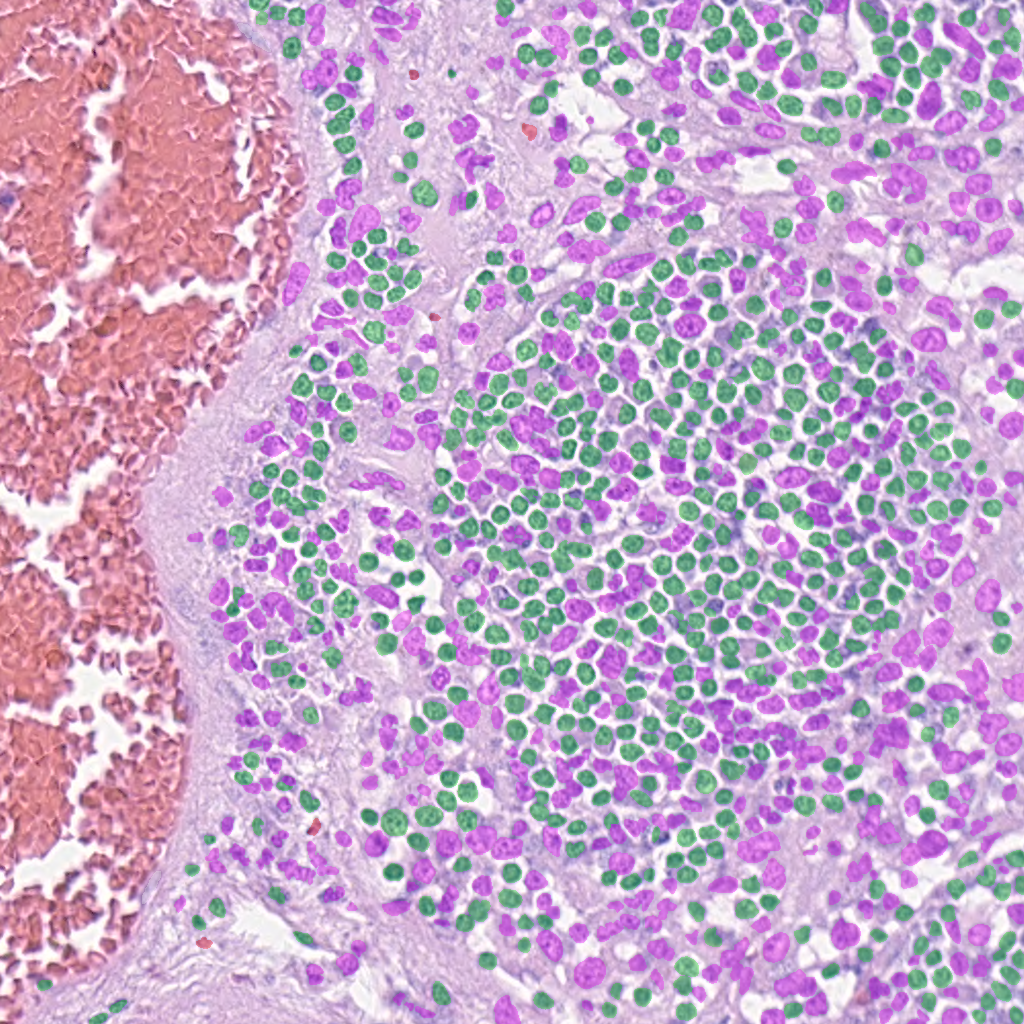
\includegraphics[width=\textwidth]{imgs/qual/consep/gt1.overlay.png}
    \caption{GT}
    \label{fig:consep-gt1}
  \end{subfigure}
  \hfill
  \begin{subfigure}[b]{0.45\textwidth}
    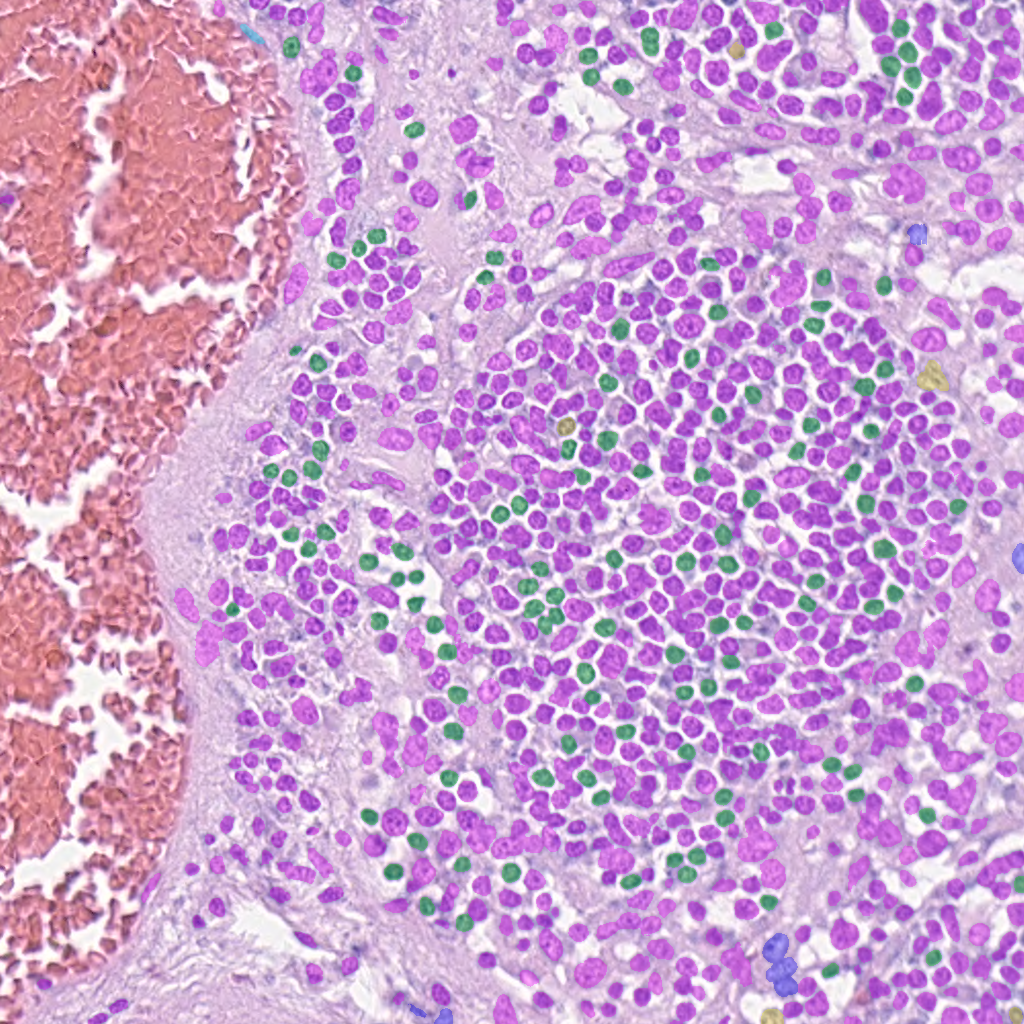
\includegraphics[width=\textwidth]{imgs/qual/consep/hov1.png}
    \caption{Hovernet}
    \label{fig:consep-hov1}
  \end{subfigure}
  \\
  \begin{subfigure}[b]{0.45\textwidth}
    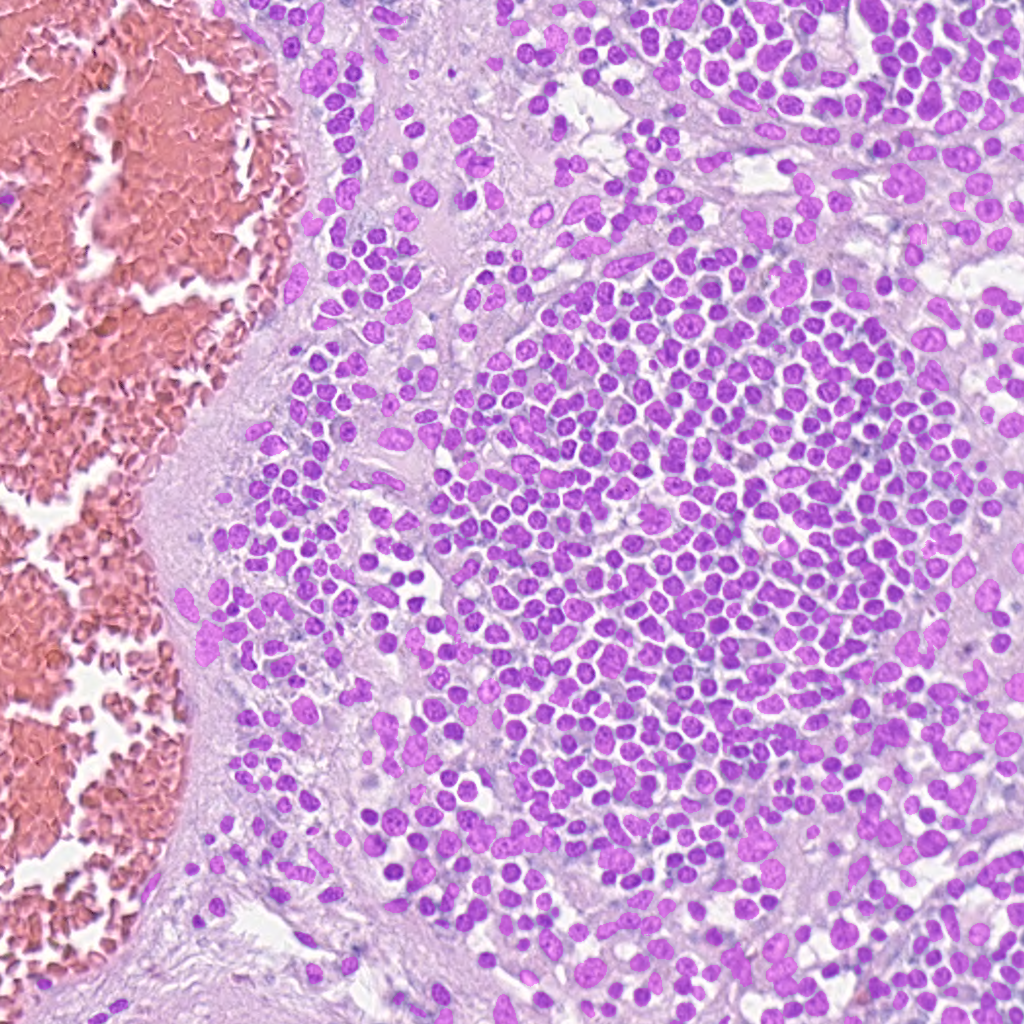
\includegraphics[width=\textwidth]{imgs/qual/consep/gcn-full1.png}
    \caption{GCN}
    \label{fig:consep-gcn1}
  \end{subfigure}
  \hfill
  \begin{subfigure}[b]{0.45\textwidth}
    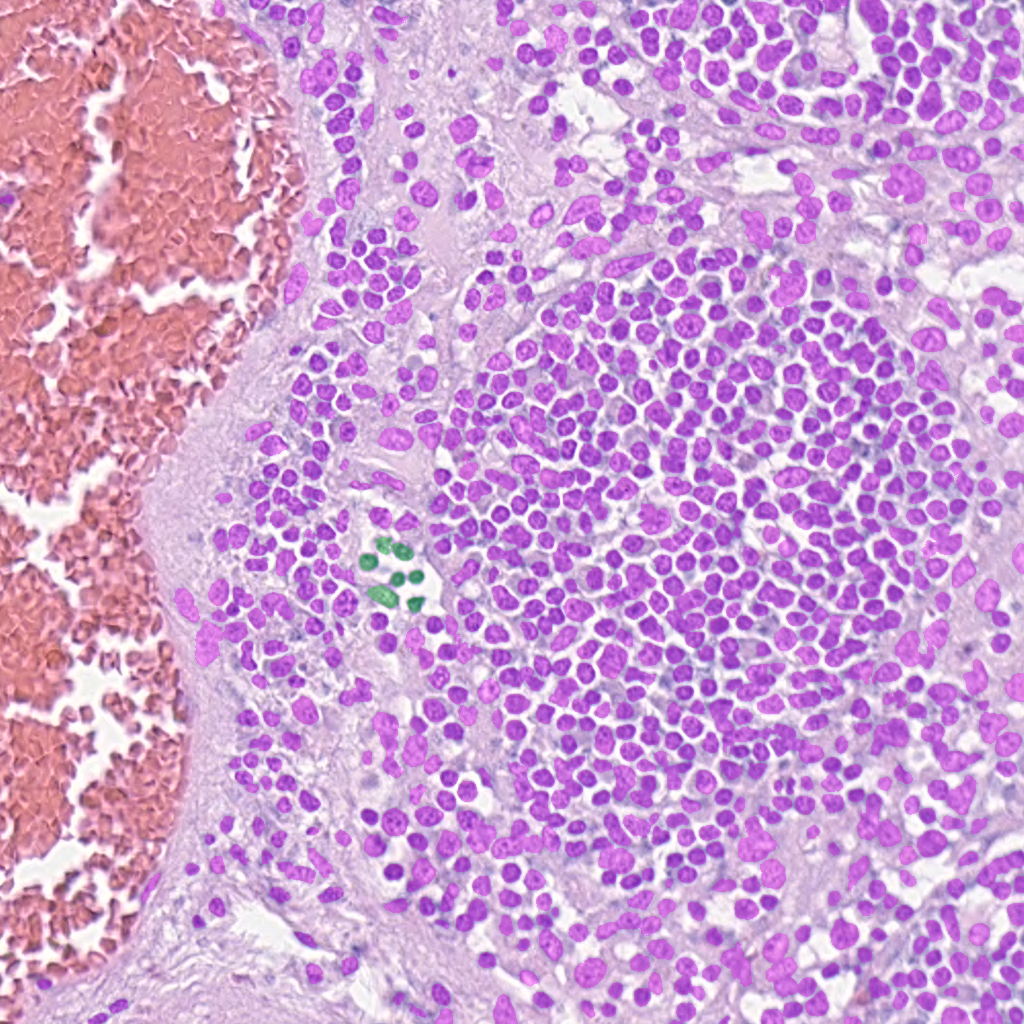
\includegraphics[width=\textwidth]{imgs/qual/consep/gat-full1.png}
    \caption{GAT}
    \label{fig:consep-gat1}
  \end{subfigure}
  \caption{Comparison of the predictions of Hovernet, graph convolution and graph attention methods.}
  \label{fig:consep-qual1}
\end{figure}

To illustrate how diverse is this concrete dataset, I will show another example where the sizes of the cells are different, the labels are different, and the way the cells are structured is also different. This example shows how difficult this dataset is. With so many classes, the number of possible ways of arranging cells is very high. Making less than 30 images not enough for the graph to learn something useful. 

\begin{figure}[H]
  \centering
  \begin{subfigure}[b]{0.45\textwidth}
    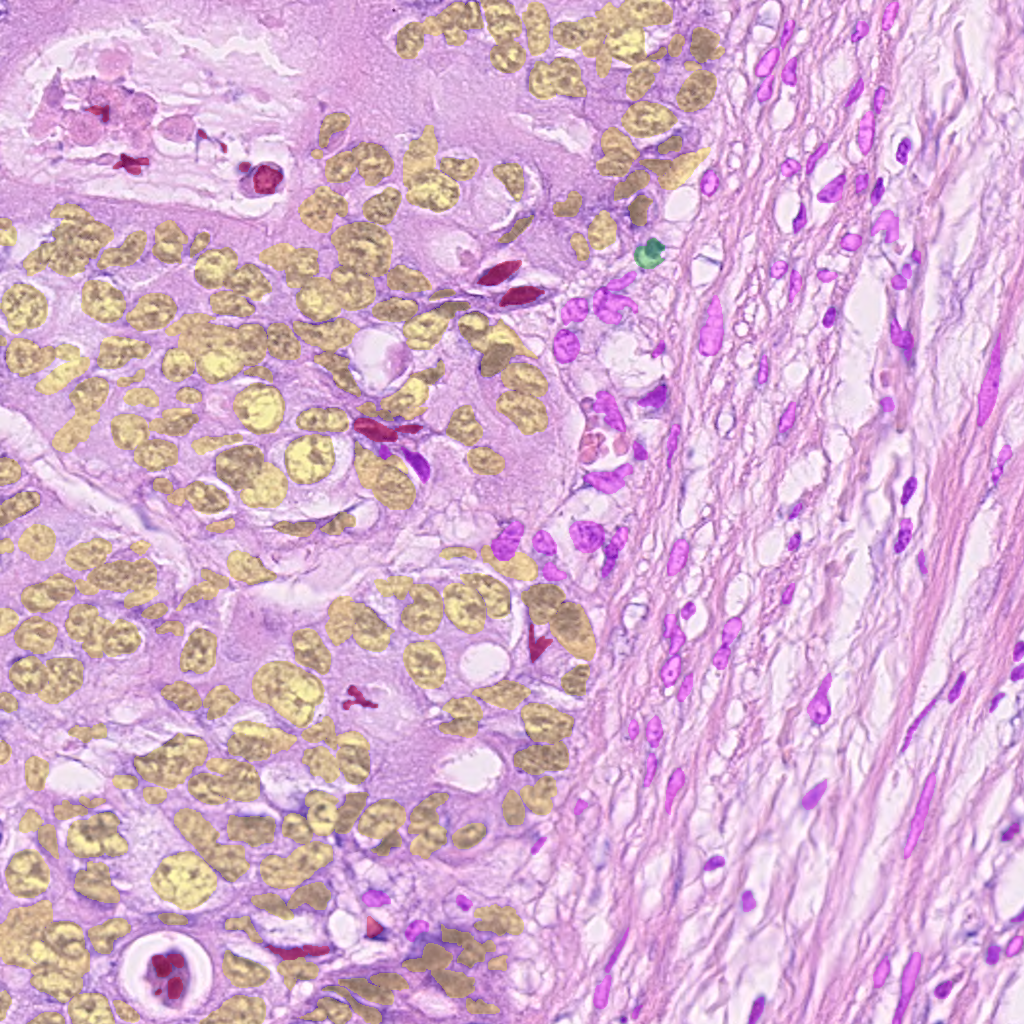
\includegraphics[width=\textwidth]{imgs/qual/consep/gt2.overlay.png}
    \caption{GT}
    \label{fig:consep-gt2}
  \end{subfigure}
  \hfill
  \begin{subfigure}[b]{0.45\textwidth}
    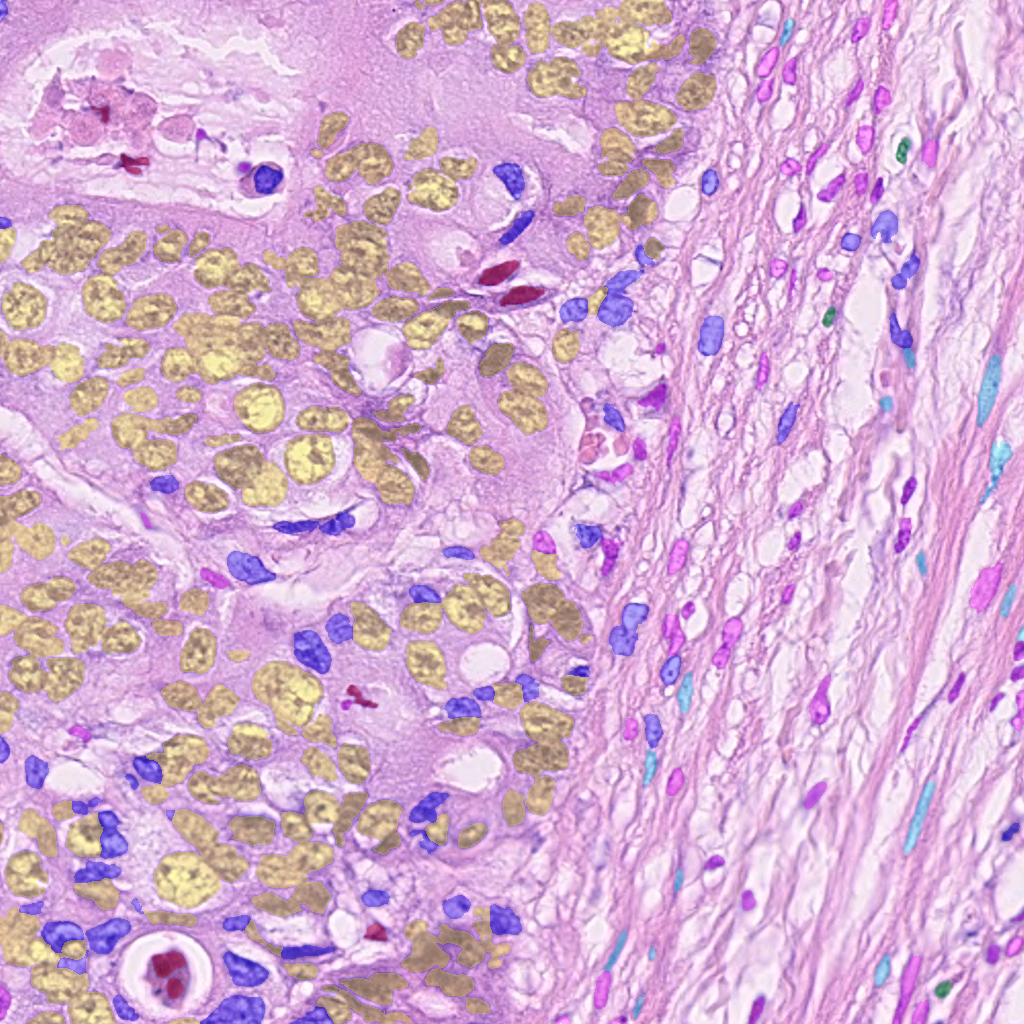
\includegraphics[width=\textwidth]{imgs/qual/consep/hov2.png}
    \caption{Hovernet}
    \label{fig:consep-hov2}
  \end{subfigure}
  \\
  \begin{subfigure}[b]{0.45\textwidth}
    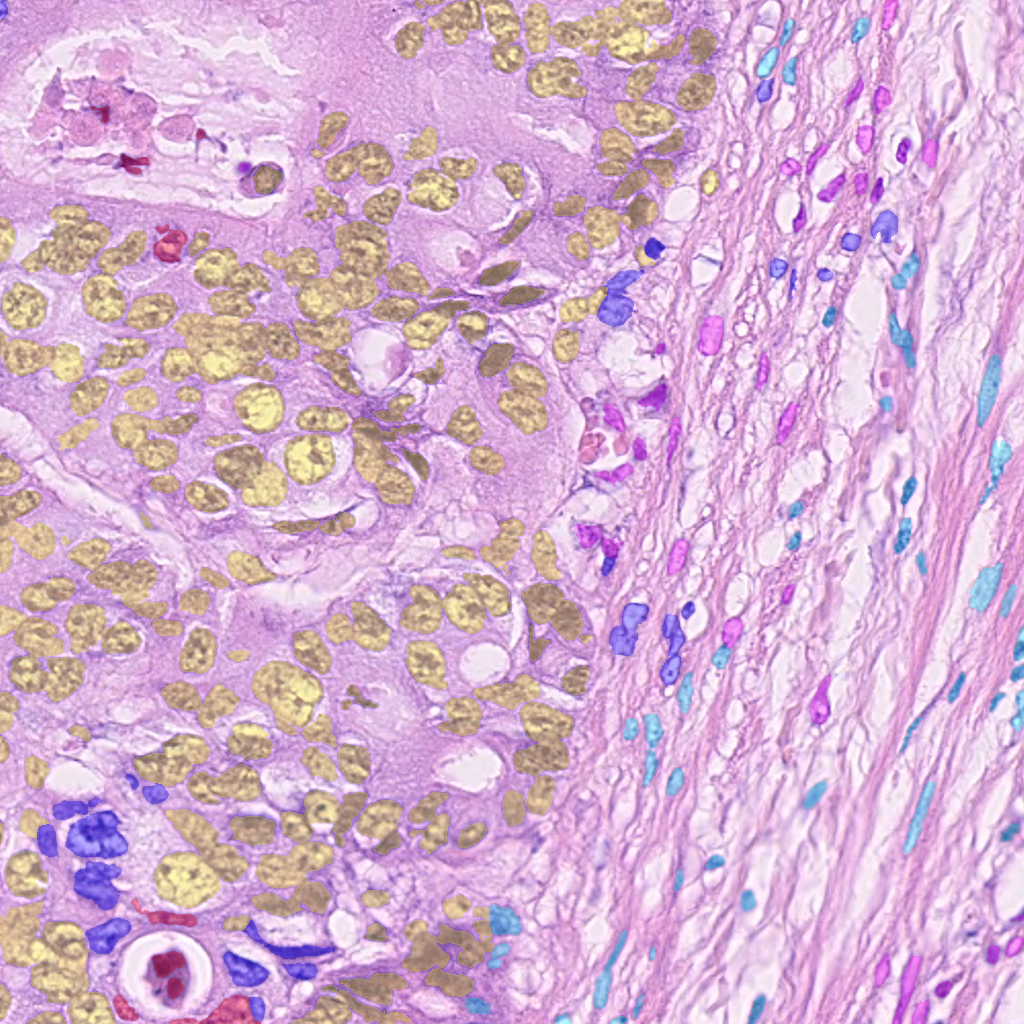
\includegraphics[width=\textwidth]{imgs/qual/consep/gcn-full2.png}
    \caption{GCN}
    \label{fig:consep-gcn2}
  \end{subfigure}
  \hfill
  \begin{subfigure}[b]{0.45\textwidth}
    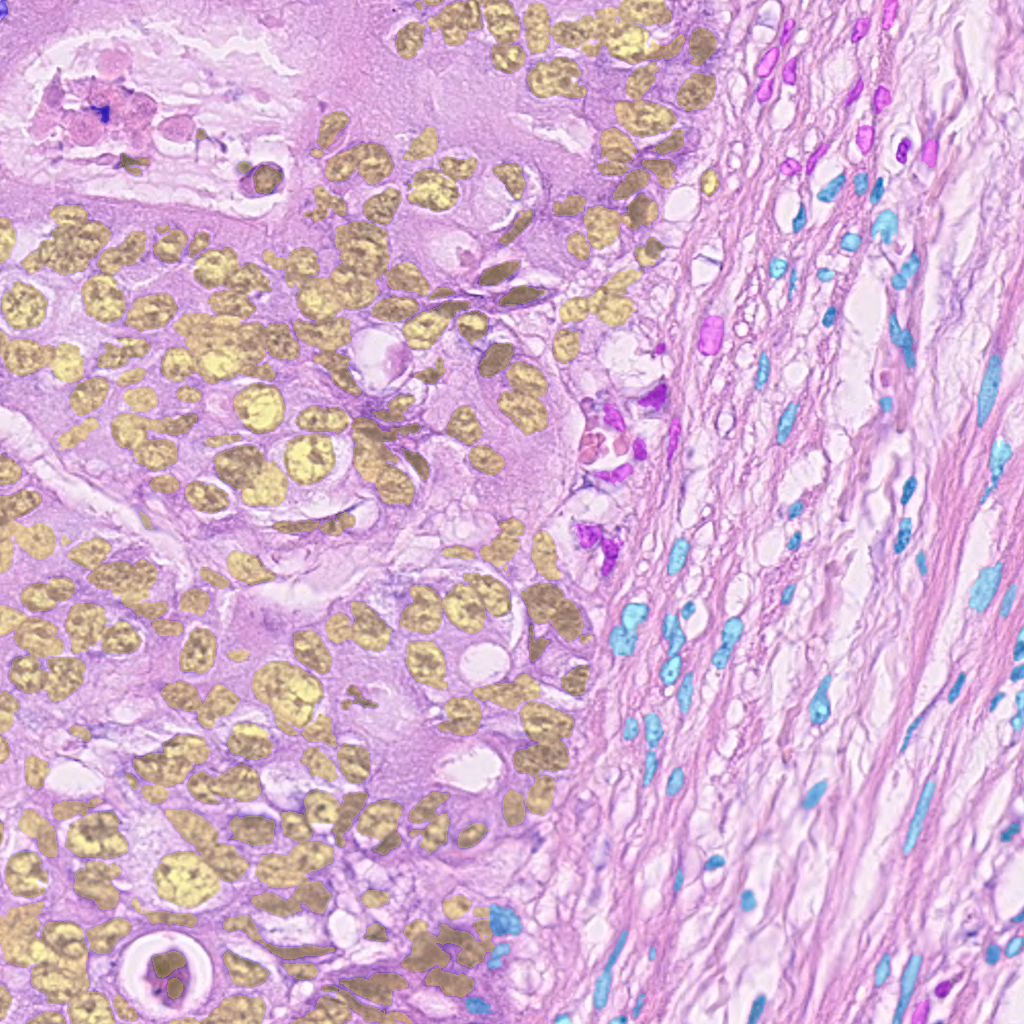
\includegraphics[width=\textwidth]{imgs/qual/consep/no-morph2.png}
    \caption{Probabilities only}
    \label{fig:consep-no-morph2}
  \end{subfigure}
  \\
  \begin{subfigure}[b]{0.45\textwidth}
    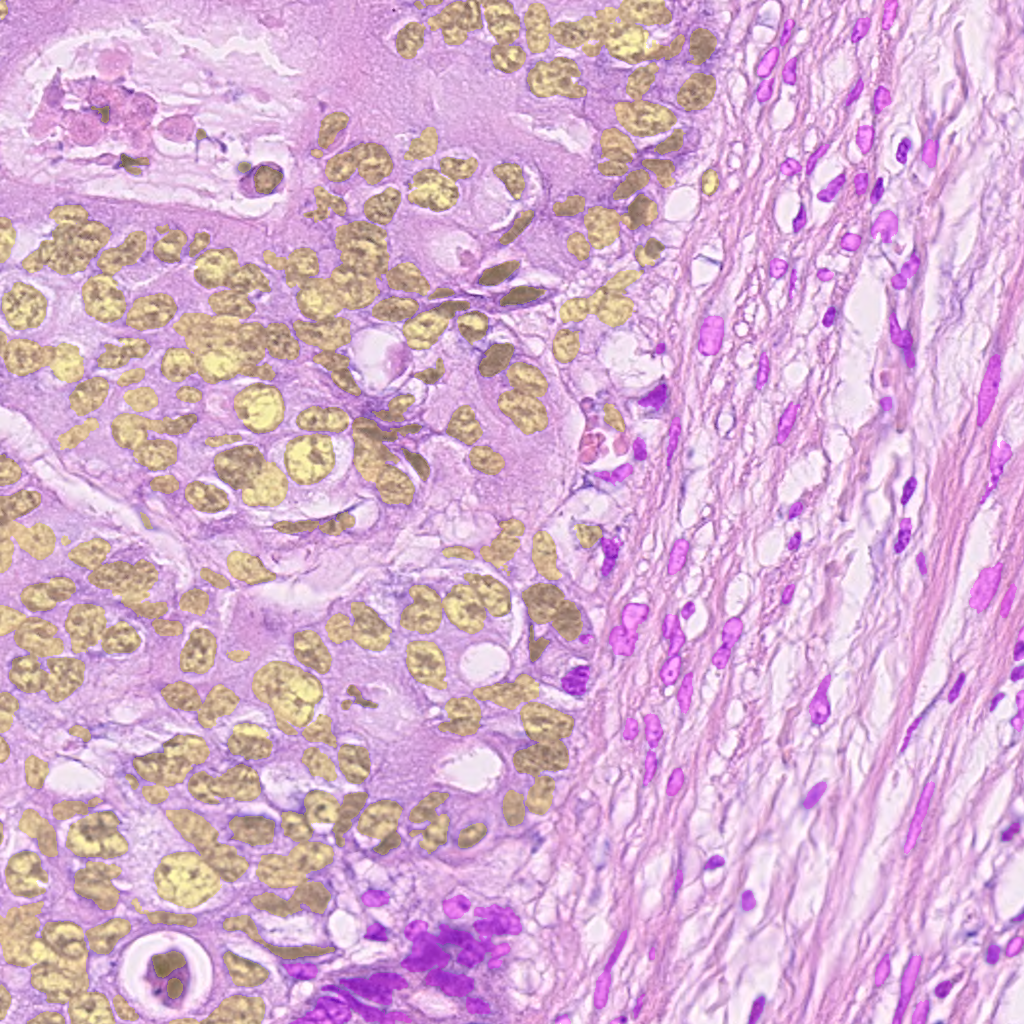
\includegraphics[width=\textwidth]{imgs/qual/consep/no-prior2.png}
    \caption{Morphological features only}
    \label{fig:consep-no-prior2}
  \end{subfigure}
  \hfill
  \begin{subfigure}[b]{0.45\textwidth}
    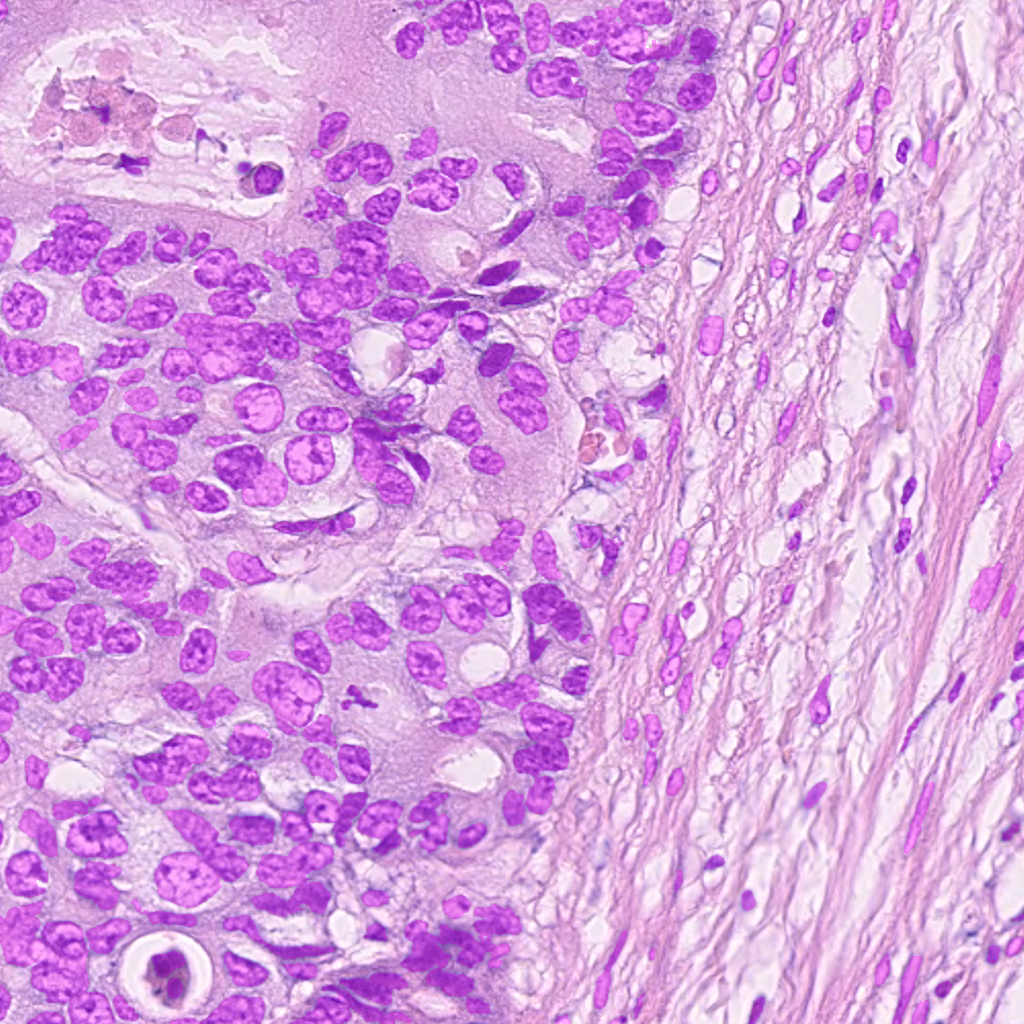
\includegraphics[width=\textwidth]{imgs/qual/consep/void2.png}
    \caption{Void}
    \label{fig:consep-void2}
  \end{subfigure}
  \caption{Illustration of the behaviour of the different models.}
  \label{fig:consep-qual2}
\end{figure}

\newpage

In \autoref{fig:consep-qual2} we can see that Hovernet misses some of the magenta cells and classifies them as blue. Here, the effect of the GCN is positive in some aspects and negative in others. The positive side is that it recovers most of the yellow cells thanks to considering them as a whole. The negative aspect is that it expands the cyan cells which were initially misclassified by Hovernet. This is a common pattern. Since the GNN operates using the probabilities from Hovernet, it can propagate the errors from it. As further proof of that look at the same example, but now look at the output from the models trained without the probabilities of Hovernet and trained only with those probabilities. The model that was trained only with probabilities further propagates the cyan group while the model trained without them did not produce any cyan cells at all. There is a trade-off when using Hovernet probabilities. It can help fix groups where Hovernet misclassified a few of the inner cells. But relying too much on Hovernet probabilities can worsen the results. When using just morphological features, the GNN is more independent from Hovernet which in this case was beneficial. Nonetheless, using no features at all is a bad idea. In this specific example the model trained only with the graph but no features classified everything as magenta, wrongly forgetting the yellow cells. Visually it is quite clear that the yellow cells and the magenta ones are a separate group, but if you just consider nodes in a graph, without indicating the area or the perimeter, there is not enough information to detect two groups in this image.

To end with the analysis of this dataset, I will display another image where cells of different types are mixed together. In \autoref{fig:consep-qual3} we can see how Hovernet predicts a more diverse set of cells than the GCN. It has yellow cells which are not surrounded by other yellow cells, it also has cyan, magenta and blue. In contrast, the GCN has mostly predicted the cyan as the dominant class. The effect of using GNNs is visible again. Hovernet takes risk and predicts lonely cells, cells with no neighbour of the same class. GNNs create neighbourhoods of cells. In this case neither of them are really a good fit since Hovernet predicts many classes that are not real and the GCN cannot really discern the mix of cyan and magenta that is in the middle of the image and predicts the whole middle group as cyan.

\begin{figure}[H]
    \centering
    \begin{subfigure}[b]{0.3\textwidth}
    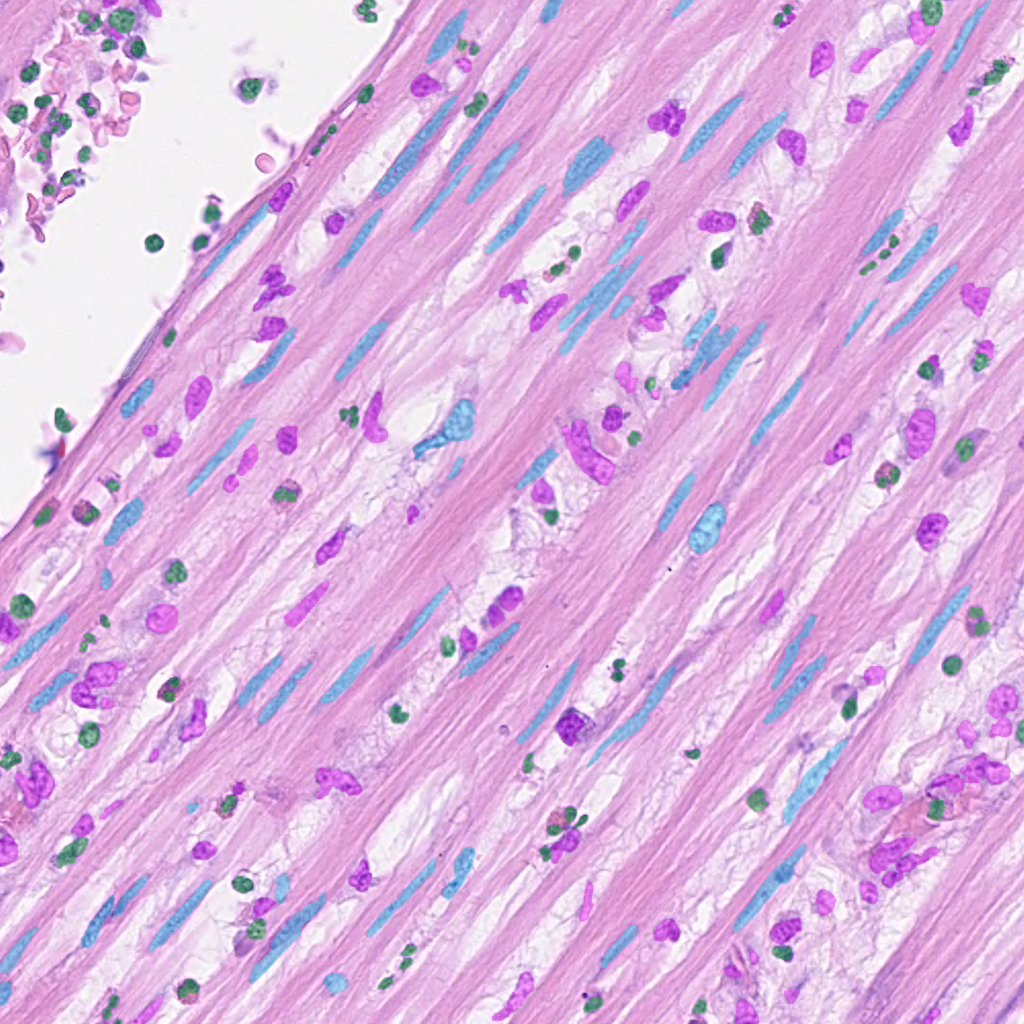
\includegraphics[width=\textwidth]{imgs/qual/consep/gt3.overlay.png}
    \caption{GT}
    \label{fig:consep-gt2}
  \end{subfigure}
  \begin{subfigure}[b]{0.3\textwidth}
    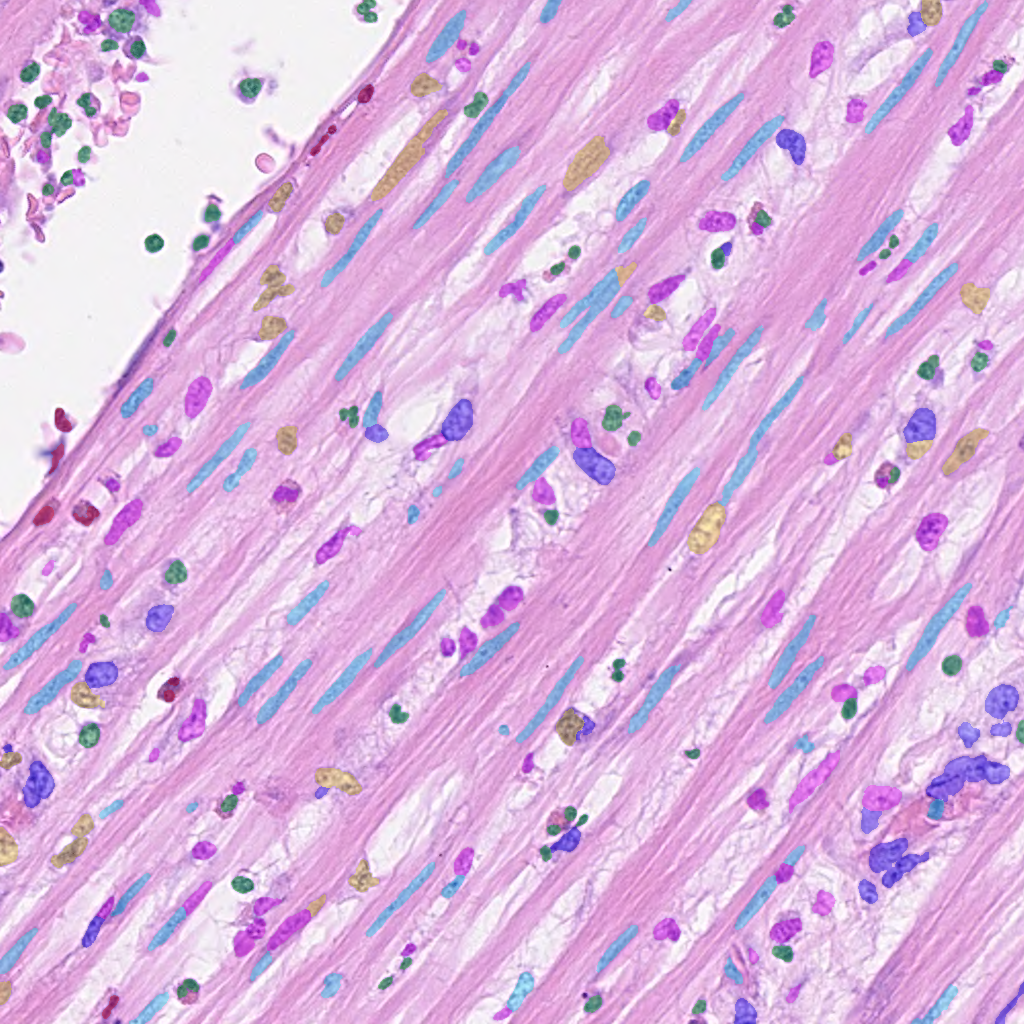
\includegraphics[width=\textwidth]{imgs/qual/consep/hov3.png}
    \caption{Hovernet}
    \label{fig:consep-hov2}
  \end{subfigure}
  \begin{subfigure}[b]{0.3\textwidth}
    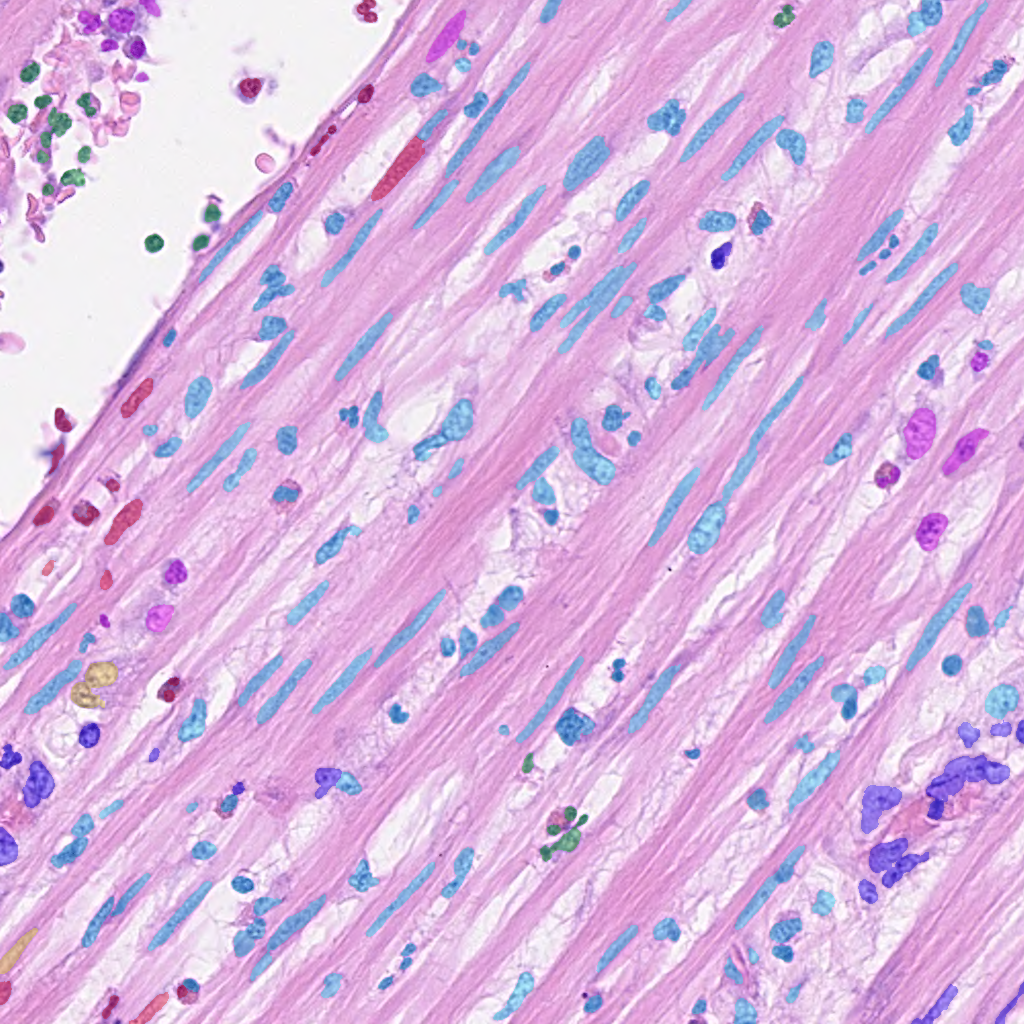
\includegraphics[width=\textwidth]{imgs/qual/consep/gcn-full3.png}
    \caption{GCN}
    \label{fig:consep-gcn2}
  \end{subfigure}
    \caption{Last example of CoNSeP database. It mixes different cell types which makes it difficult for the GNN to work properly.}
    \label{fig:consep-qual3}
\end{figure}

\newpage
\subsection{MoNuSAC}

In previous sections I have stated that this dataset was a good example of where the graph neural networks are a good fit. With the CoNSeP dataset we have seen that those models tend to group cell togethers. When there is a mix of different classes it works poorly. In \autoref{fig:monusac-ex} we can see three examples out of this dataset which are exactly the opposite. They contain well defined groups. It is difficult to appreciate but in the image on the left there are two well defined groups, one green and one red and in the image at the left there are also blue cells close to each other. Many of the images in this dataset are like the one in the middle, with only one class in the whole image. Having this setup it is expected to see Hovernet misclassify some cells since it is not considering the image as a whole while the GNNs solve that problem by merging everything into big groups.

\begin{figure}[H]
    \centering
    \begin{subfigure}[b]{0.3\textwidth}
    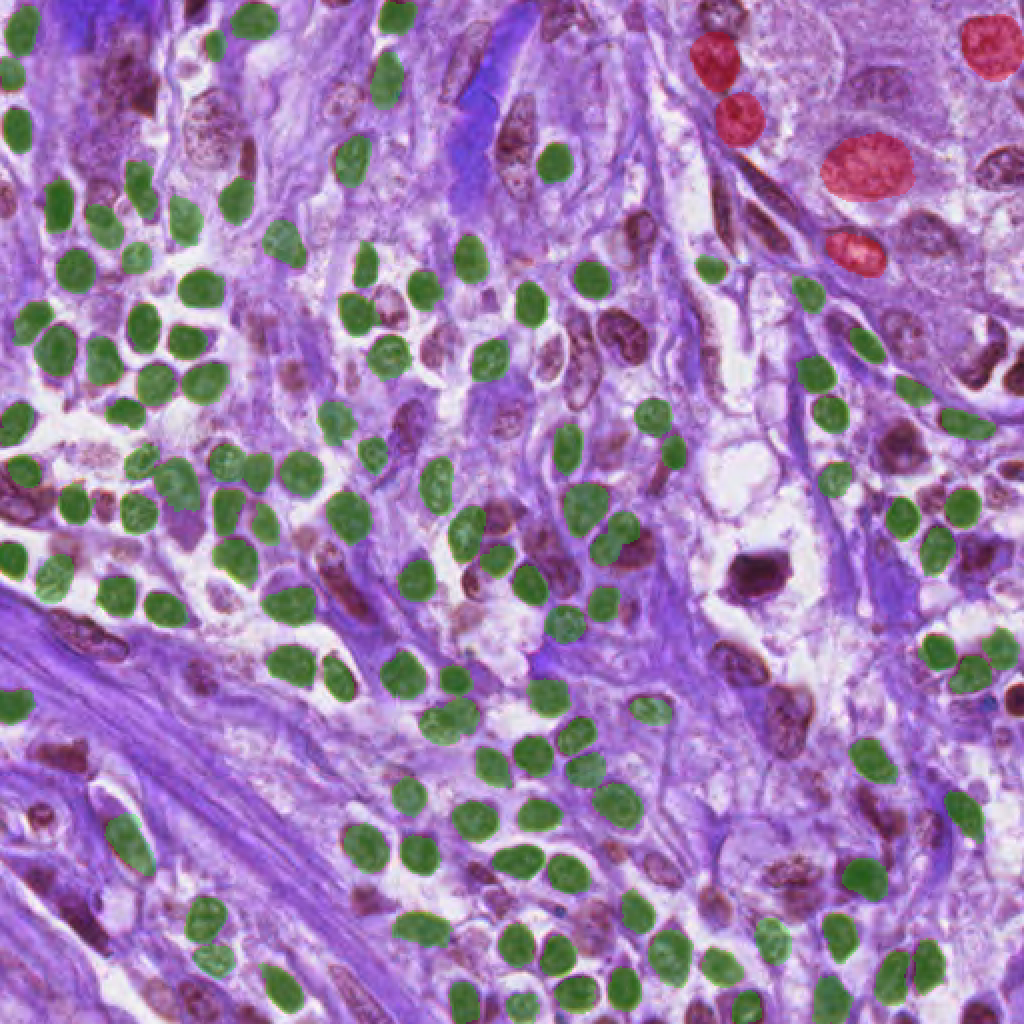
\includegraphics[width=\textwidth]{imgs/qual/monusac/gt1.overlay.png}
    \label{fig:monusac-gt1}
  \end{subfigure}
  \begin{subfigure}[b]{0.3\textwidth}
    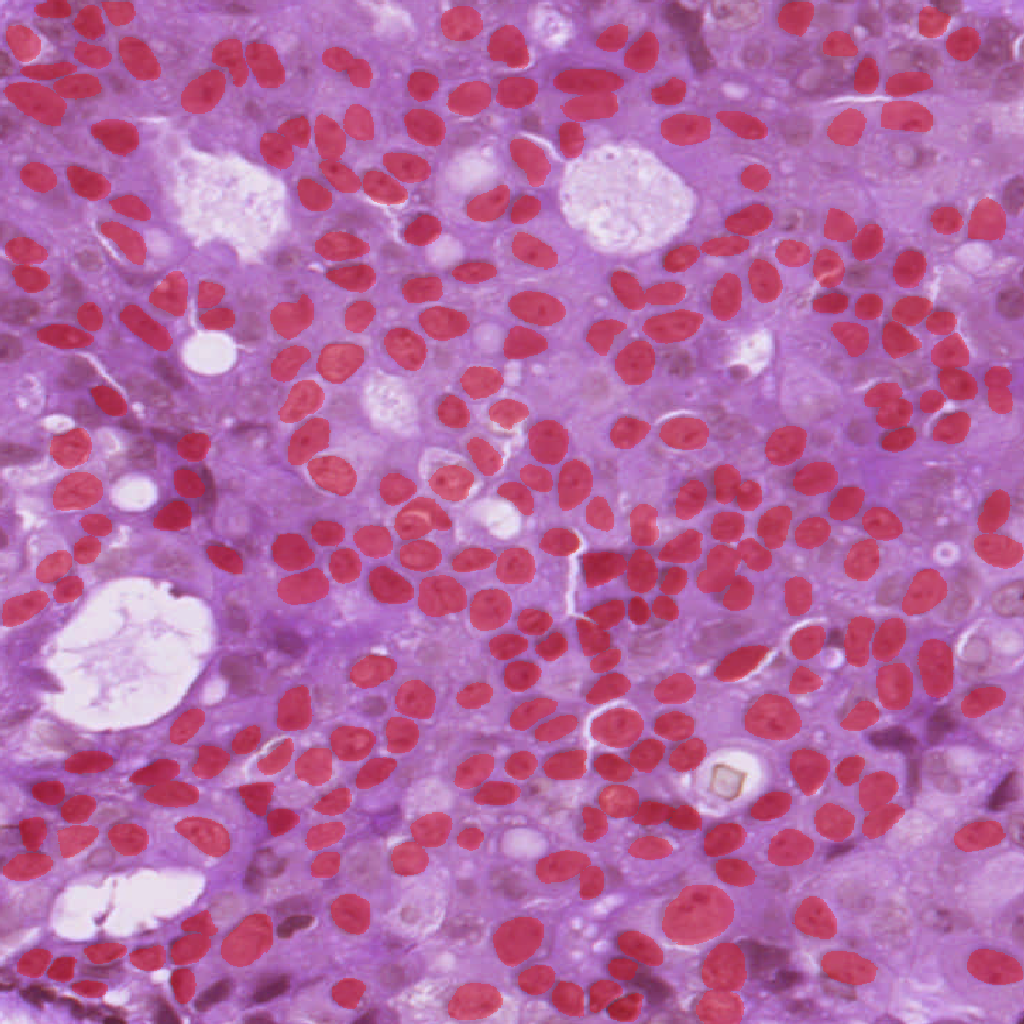
\includegraphics[width=\textwidth]{imgs/qual/monusac/gt2.overlay.png}
    \label{fig:monusac-gt2}
  \end{subfigure}
  \begin{subfigure}[b]{0.3\textwidth}
    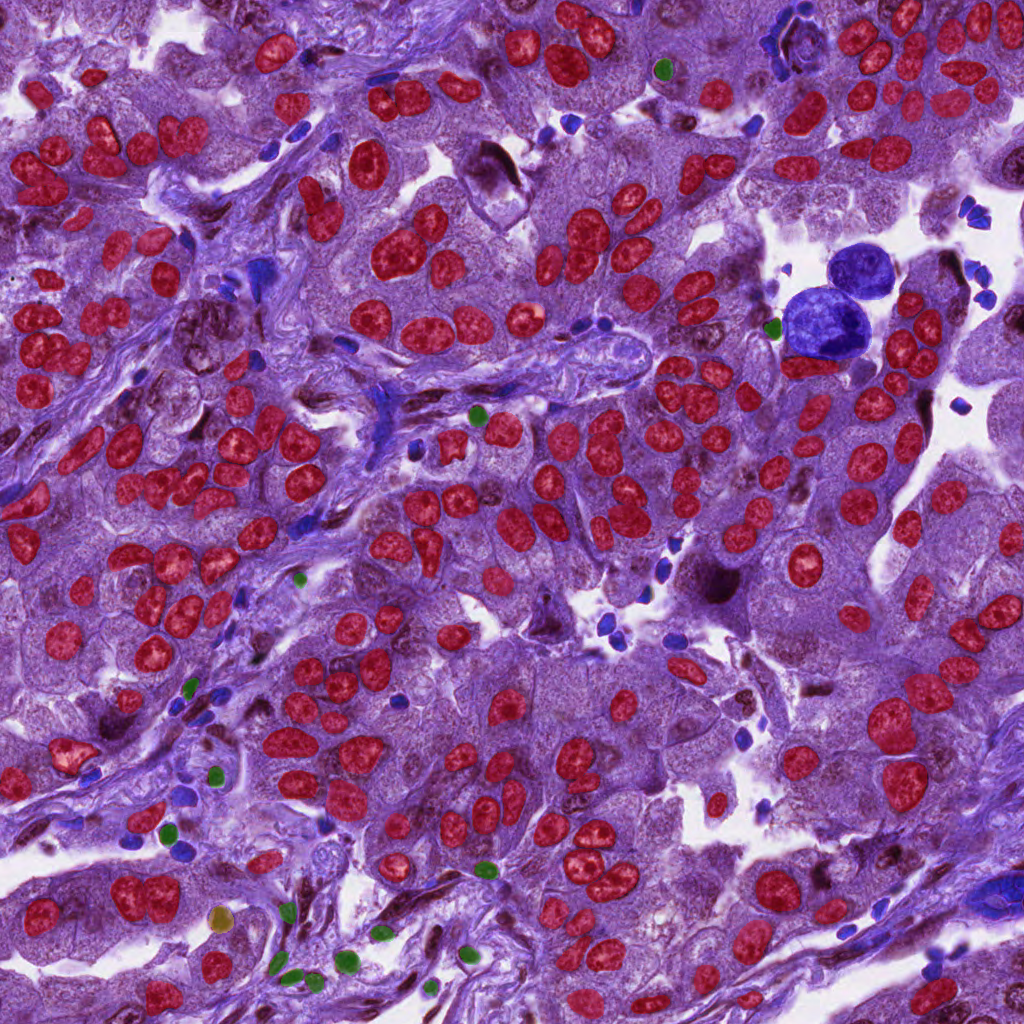
\includegraphics[width=\textwidth]{imgs/qual/monusac/gt3.overlay.png}
    \label{fig:monusac-gt3}
  \end{subfigure}
    \caption{Three examples with their ground truth overlayed on top.}
    \label{fig:monusac-ex}
\end{figure}

Let's dive into the details of what every model predicted with the image on the left. Same as what happened in CoNSeP, here in \autoref{fig:monusac-qual1} the Hovernet randomly misclassifies some green cells into red cells. The graph network that was trained only with Hovernet probabilities believes it and so it creates three nests. The green in the middle, the red at the top right and the red at the bottom left grouping and merging the result from the Hovernet. The network trained with morphological features is more correct in that the group at the bottom left is correctly classified as green while preserving the red group at the top right. The GCN trained with everything is confused and so it simply predicts everything as green. Finally, the GCN that only sees the graph and no features at all behaves a bit unpredictably, creating another group of red cells at the bottom right and at the top left.

Similar conclusions can be drawn with the result obtained from the image on the right of \autoref{fig:monusac-ex}. The output is on \autoref{fig:monusac-qual3}. The result with the remaining image at the center of \autoref{fig:monusac-ex} is less informative. In there all the models correctly predicted every cell as red. Even though Hovernet sometimes randomly misclassifies little cells, there are cases like the one in the middle of \autoref{fig:monusac-ex} that everything is correctly classified. When there is only one group to classify, the graph networks will be as right as Hovernet. After all, they are using the probabilities as inputs and creating clusters of cells. If there is only one cluster, there is not much work to do.

\begin{figure}[H]
  \centering
  \begin{subfigure}[b]{0.45\textwidth}
    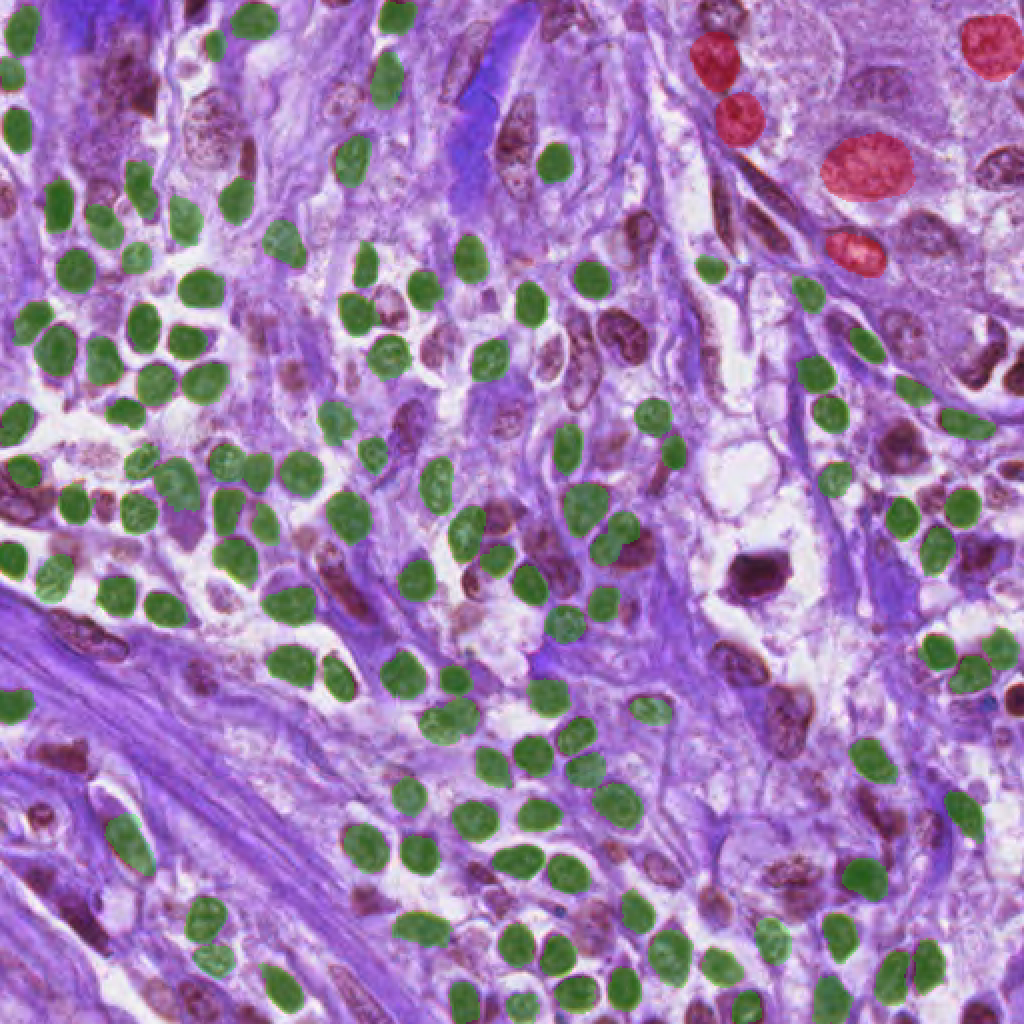
\includegraphics[width=\textwidth]{imgs/qual/monusac/gt1.overlay.png}
    \caption{GT}
    \label{fig:monusac-gt1}
  \end{subfigure}
  \hfill
  \begin{subfigure}[b]{0.45\textwidth}
    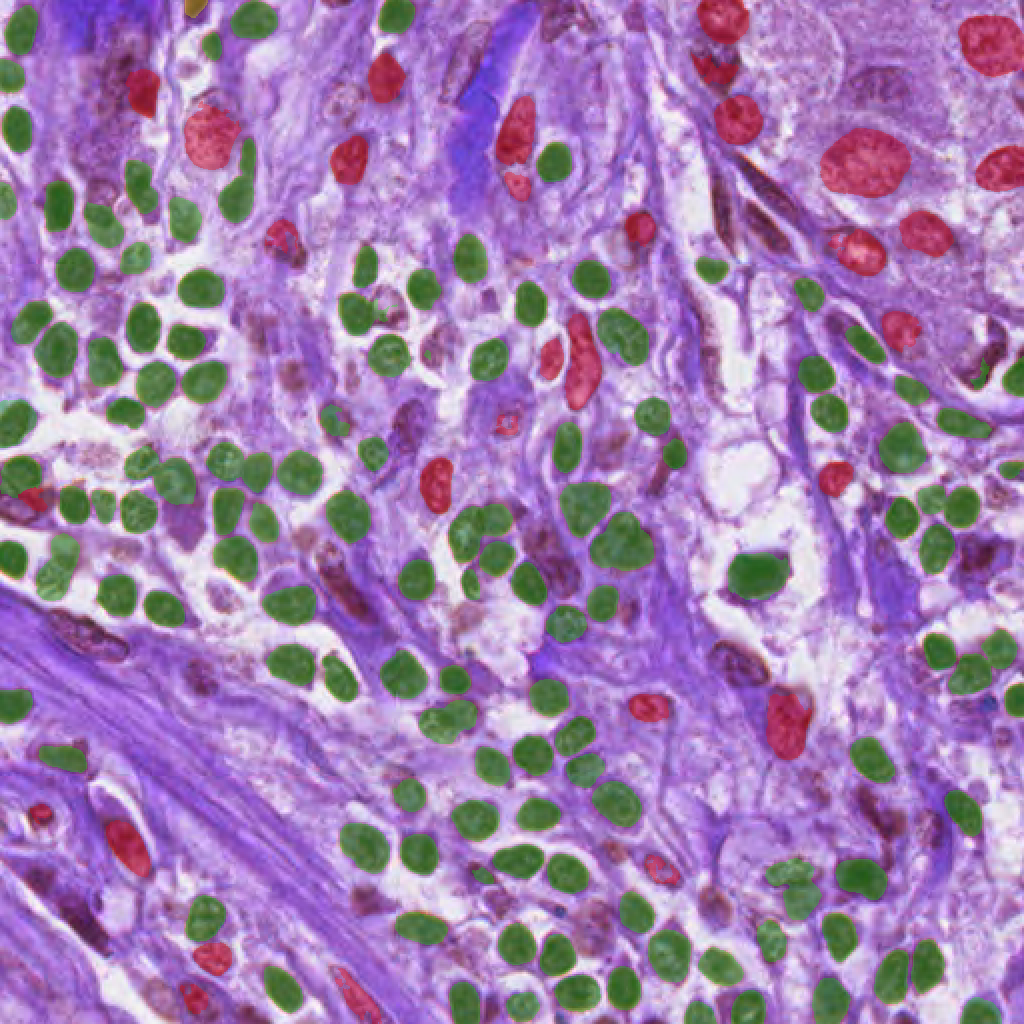
\includegraphics[width=\textwidth]{imgs/qual/monusac/hov1.png}
    \caption{Hovernet}
    \label{fig:monusac-hov1}
  \end{subfigure}
  \\
  \begin{subfigure}[b]{0.45\textwidth}
    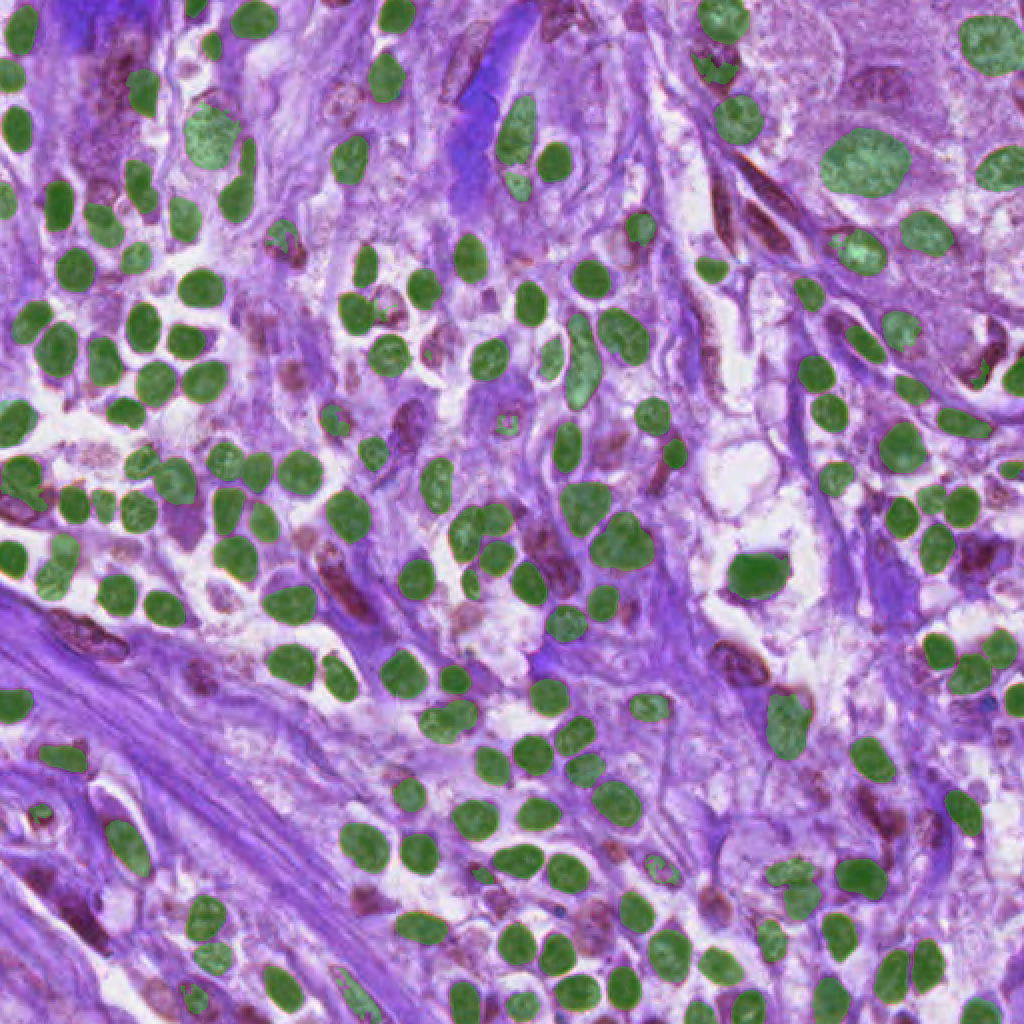
\includegraphics[width=\textwidth]{imgs/qual/monusac/gcn-full1.png}
    \caption{GCN}
    \label{fig:monusac-gcn1}
  \end{subfigure}
  \hfill
  \begin{subfigure}[b]{0.45\textwidth}
    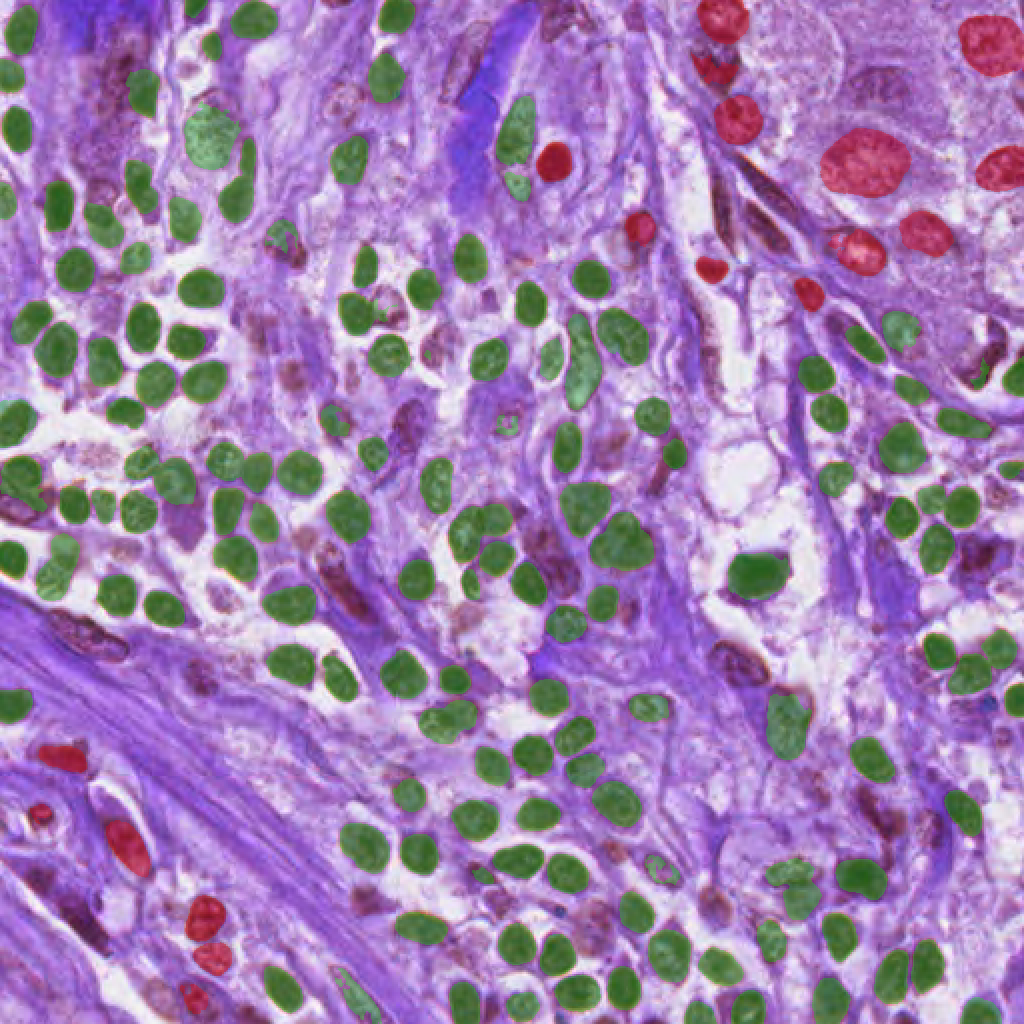
\includegraphics[width=\textwidth]{imgs/qual/monusac/no-morph1.png}
    \caption{Probabilities only}
    \label{fig:monusac-no-morph1}
  \end{subfigure}
  \\
  \begin{subfigure}[b]{0.45\textwidth}
    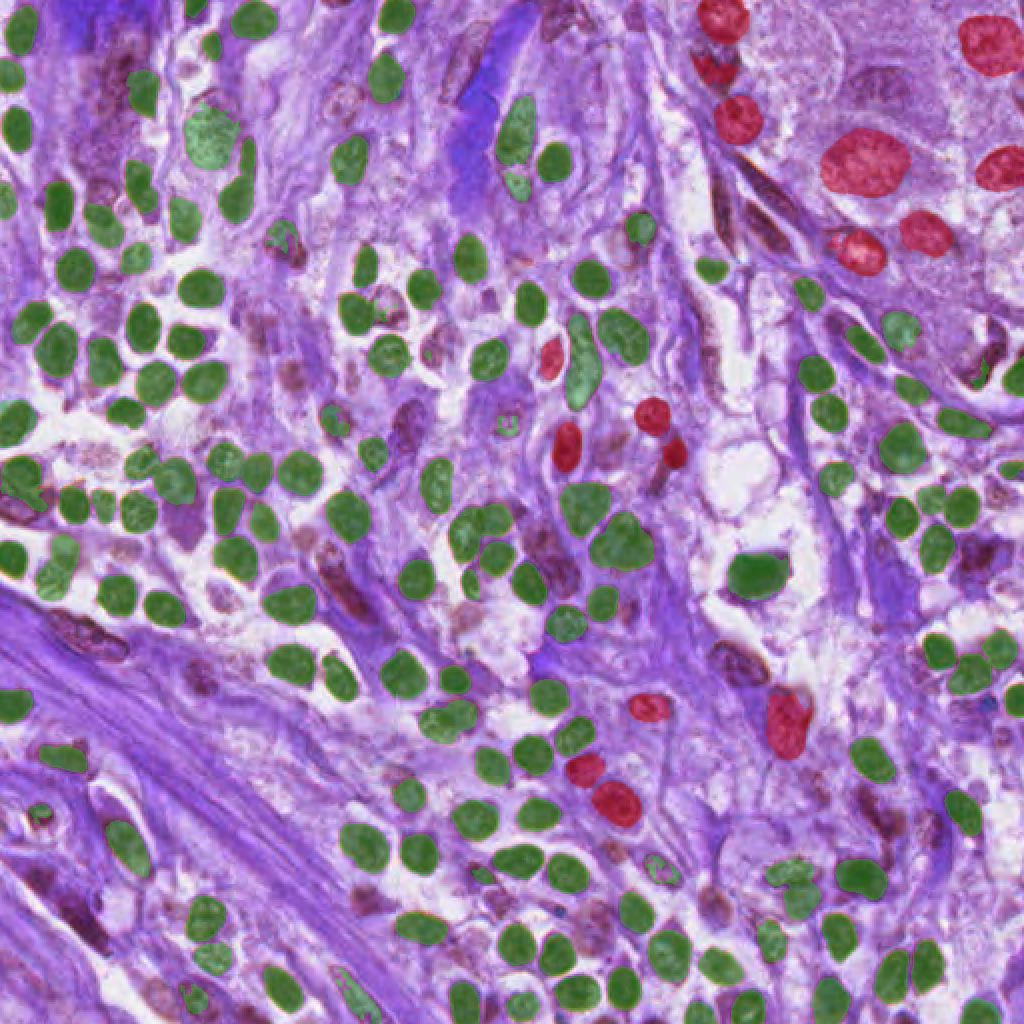
\includegraphics[width=\textwidth]{imgs/qual/monusac/no-prior1.png}
    \caption{Morphological features only}
    \label{fig:monusac-no-prior1}
  \end{subfigure}
  \hfill
  \begin{subfigure}[b]{0.45\textwidth}
    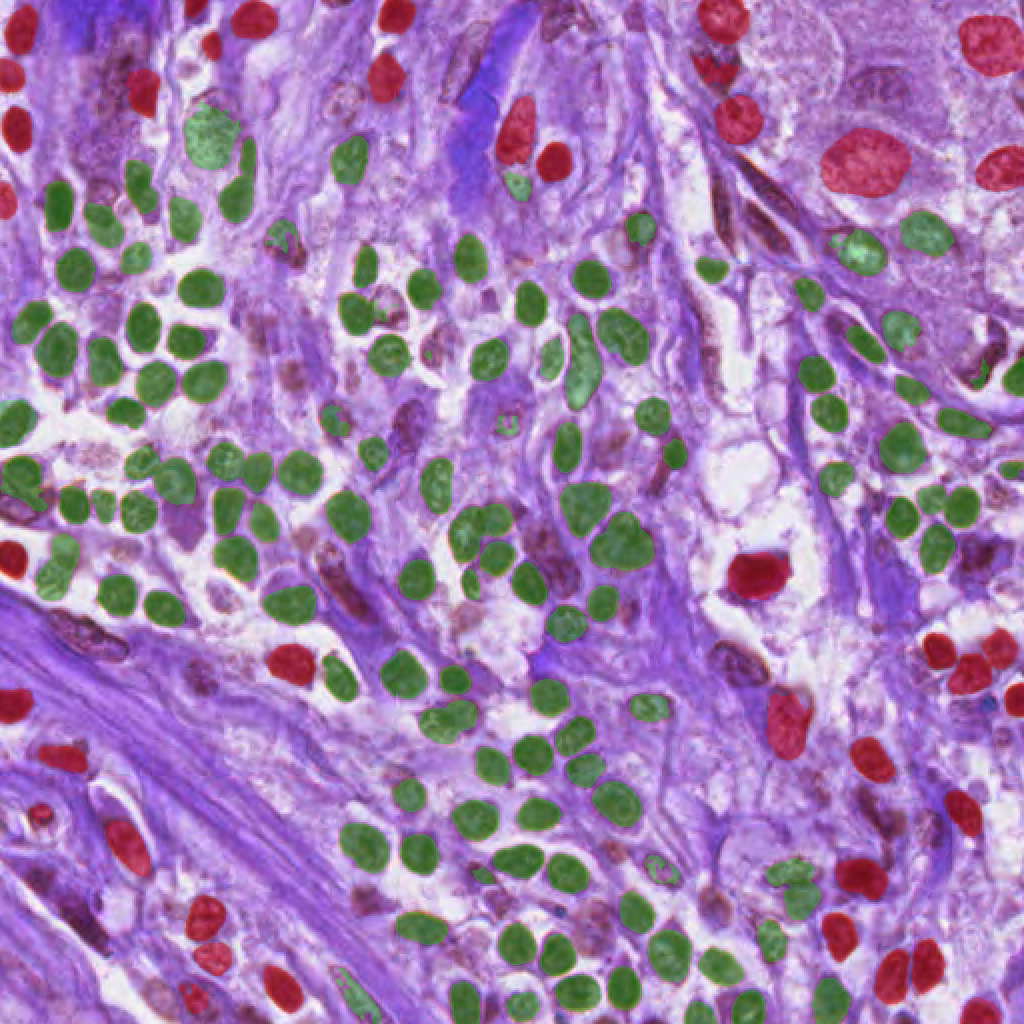
\includegraphics[width=\textwidth]{imgs/qual/monusac/void1.png}
    \caption{Void}
    \label{fig:monusac-void1}
  \end{subfigure}
  \caption{Illustration of the behaviour of the different models.}
  \label{fig:monusac-qual1}
\end{figure}

\begin{figure}[H]
  \centering
  \begin{subfigure}[b]{0.45\textwidth}
    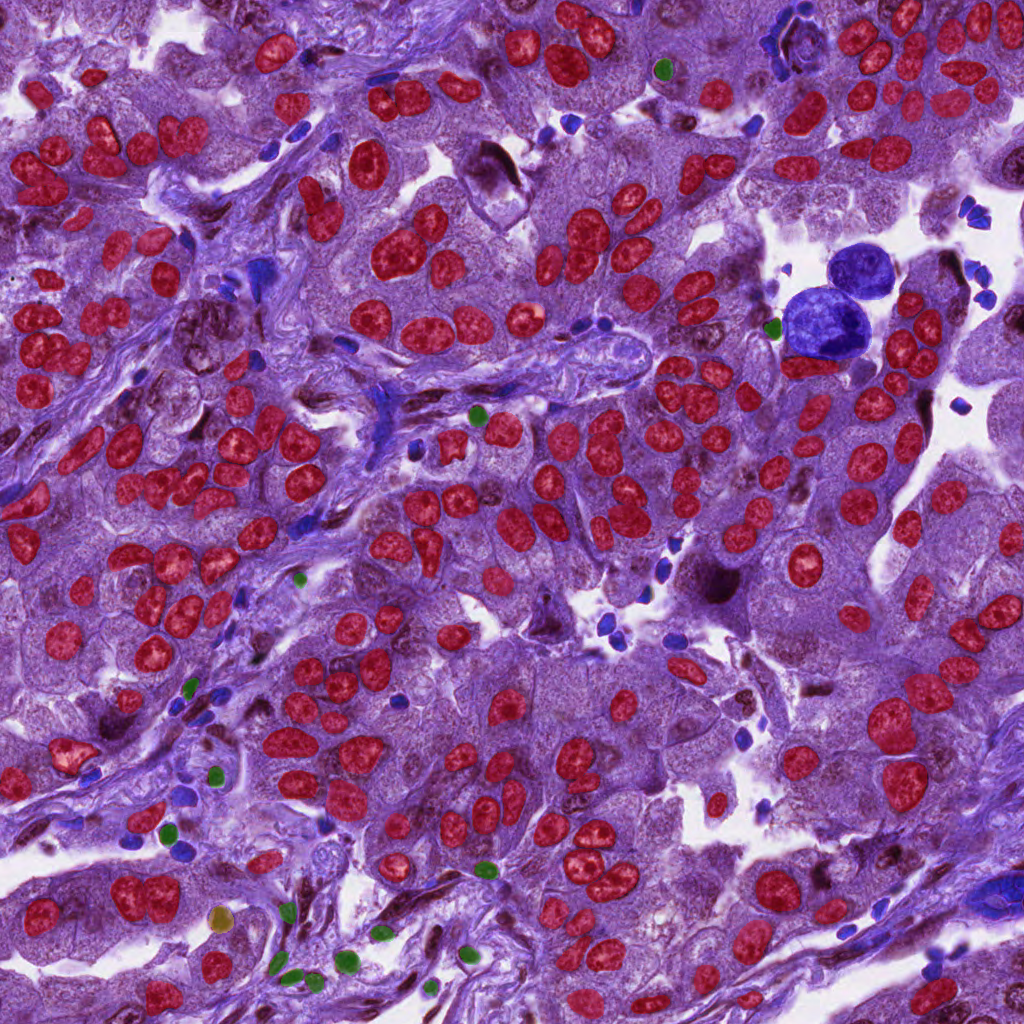
\includegraphics[width=\textwidth]{imgs/qual/monusac/gt3.overlay.png}
    \caption{GT}
    \label{fig:monusac-gt3}
  \end{subfigure}
  \hfill
  \begin{subfigure}[b]{0.45\textwidth}
    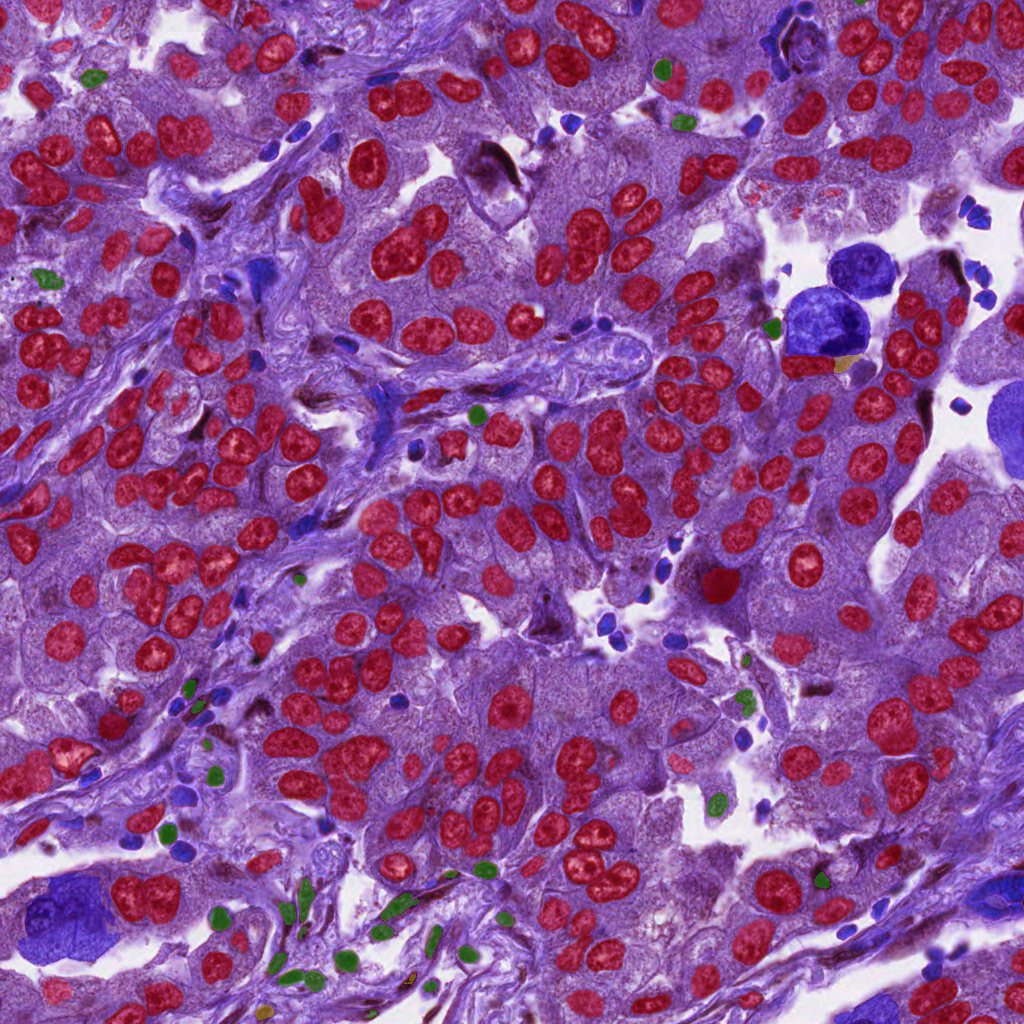
\includegraphics[width=\textwidth]{imgs/qual/monusac/hov3.png}
    \caption{Hovernet}
    \label{fig:monusac-hov3}
  \end{subfigure}
  \\
  \begin{subfigure}[b]{0.45\textwidth}
    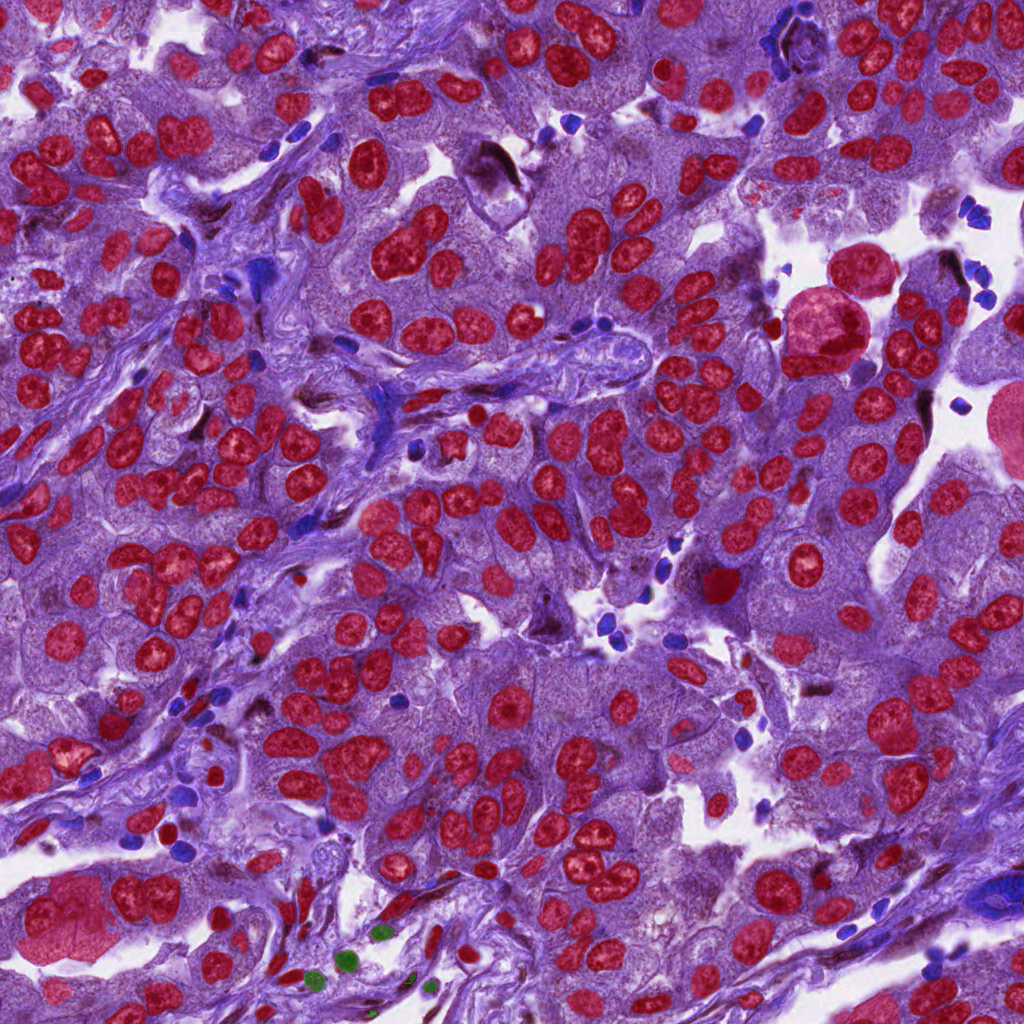
\includegraphics[width=\textwidth]{imgs/qual/monusac/gcn-full3.png}
    \caption{GCN}
    \label{fig:monusac-gcn3}
  \end{subfigure}
  \hfill
  \begin{subfigure}[b]{0.45\textwidth}
    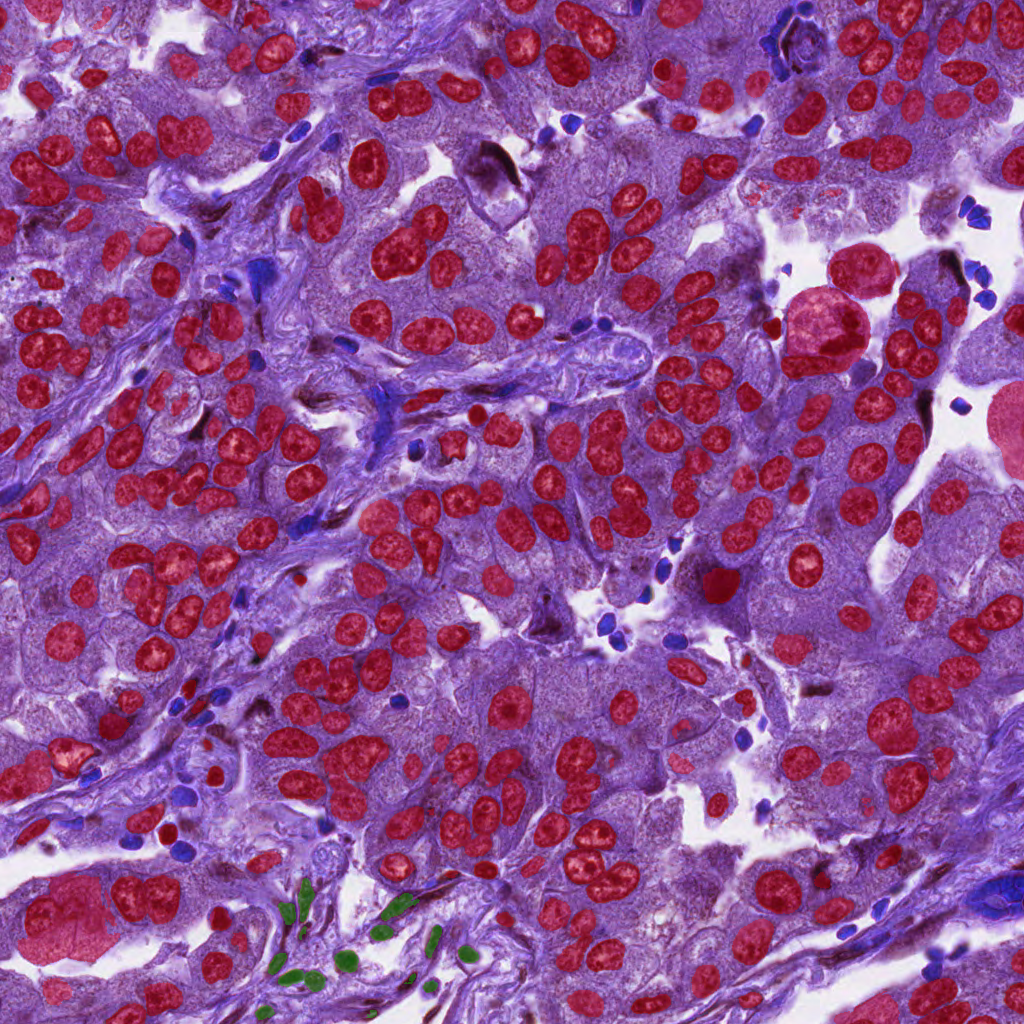
\includegraphics[width=\textwidth]{imgs/qual/monusac/no-morph3.png}
    \caption{Probabilities only}
    \label{fig:monusac-no-morph3}
  \end{subfigure}
  \\
  \begin{subfigure}[b]{0.45\textwidth}
    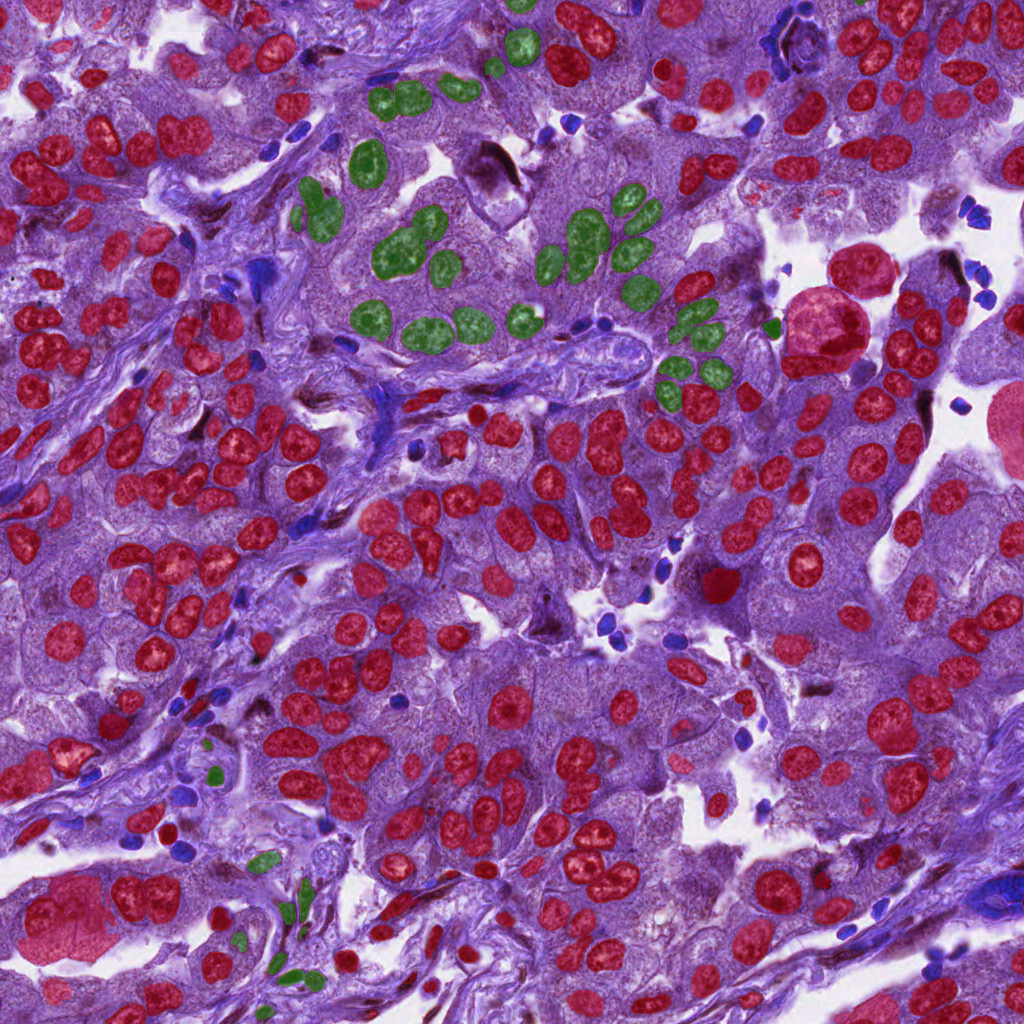
\includegraphics[width=\textwidth]{imgs/qual/monusac/no-prior3.png}
    \caption{Morphological features only}
    \label{fig:monusac-no-prior3}
  \end{subfigure}
  \hfill
  \begin{subfigure}[b]{0.45\textwidth}
    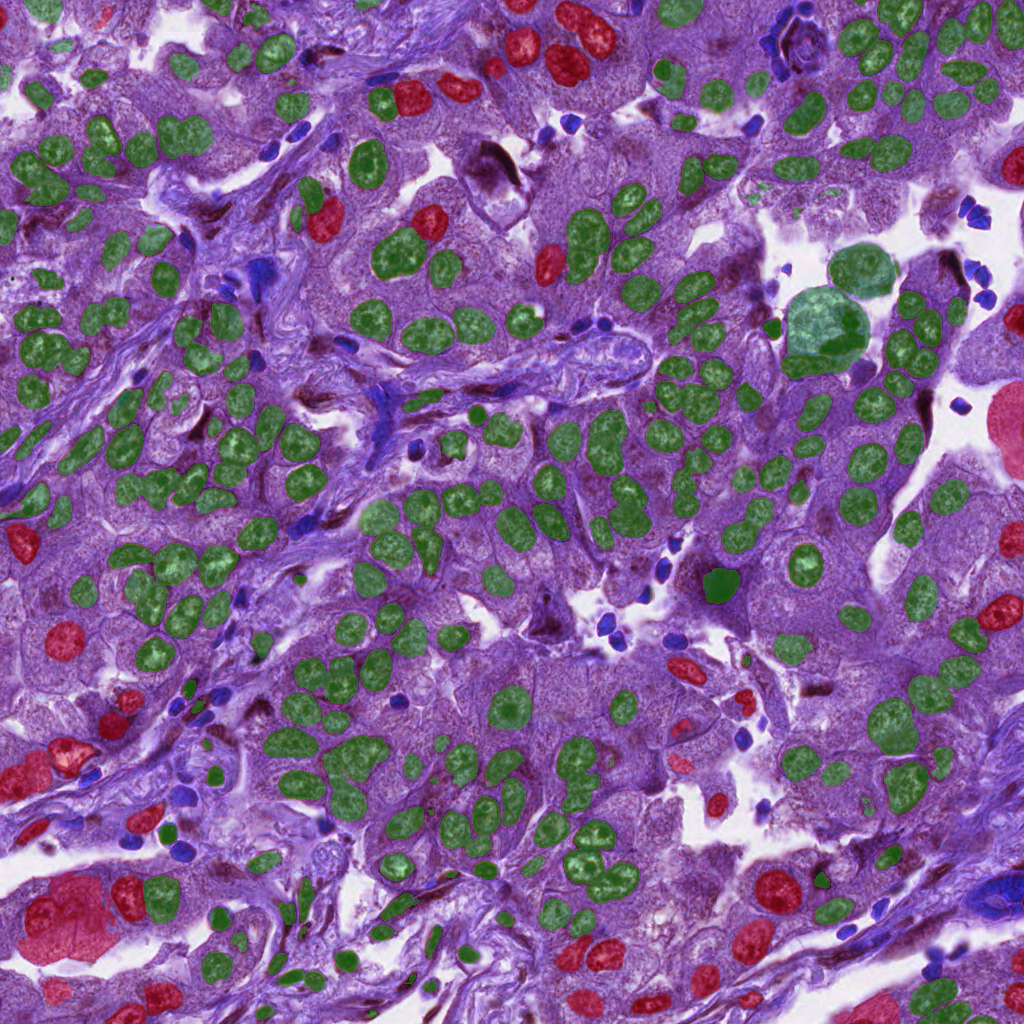
\includegraphics[width=\textwidth]{imgs/qual/monusac/void3.png}
    \caption{Void}
    \label{fig:monusac-void3}
  \end{subfigure}
  \caption{Another illustration of the behaviour of the different models.}
  \label{fig:monusac-qual3}
\end{figure}


\subsection{DigiPatics breast}

Let's start the qualitative analysis of this section with a question. Given the following three images with their ground truth on top. Which of them would you think is going to give less trouble to the graph neural networks? If you have read the previous two sections the answer should be obvious by now.

\begin{figure}[H]
    \centering
    \begin{subfigure}[b]{0.3\textwidth}
    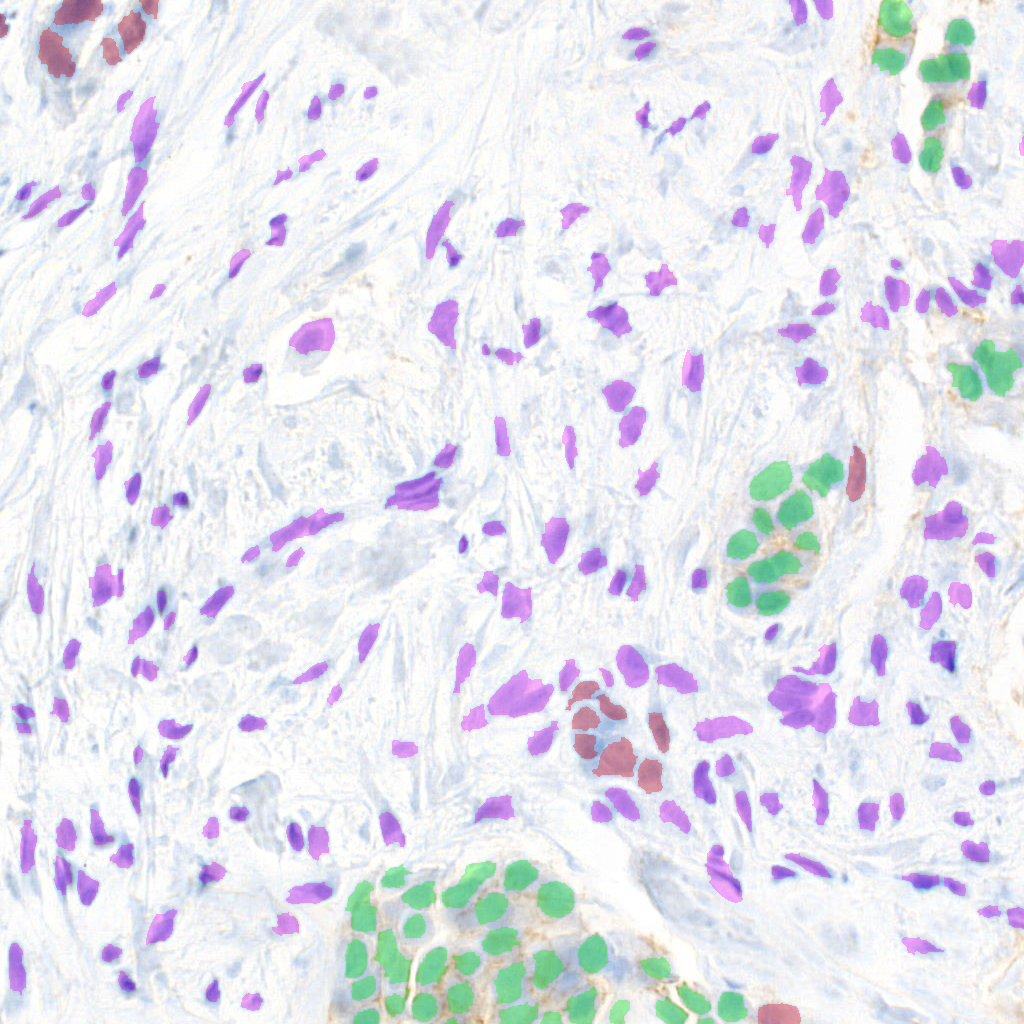
\includegraphics[width=\textwidth]{imgs/qual/breast/gt1.overlay.png}
    \label{fig:breast-gt1}
  \end{subfigure}
  \begin{subfigure}[b]{0.3\textwidth}
    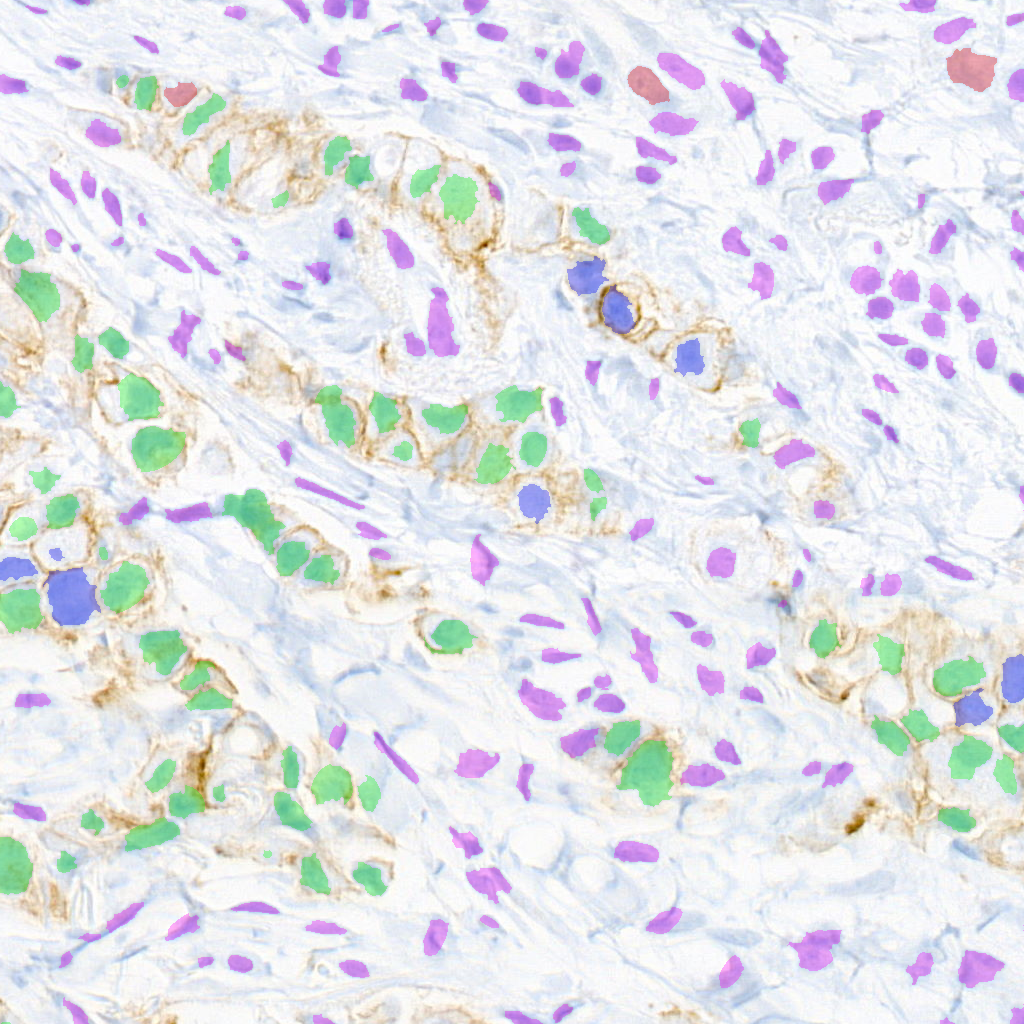
\includegraphics[width=\textwidth]{imgs/qual/breast/gt2.overlay.png}
    \label{fig:breast-gt2}
  \end{subfigure}
  \begin{subfigure}[b]{0.3\textwidth}
    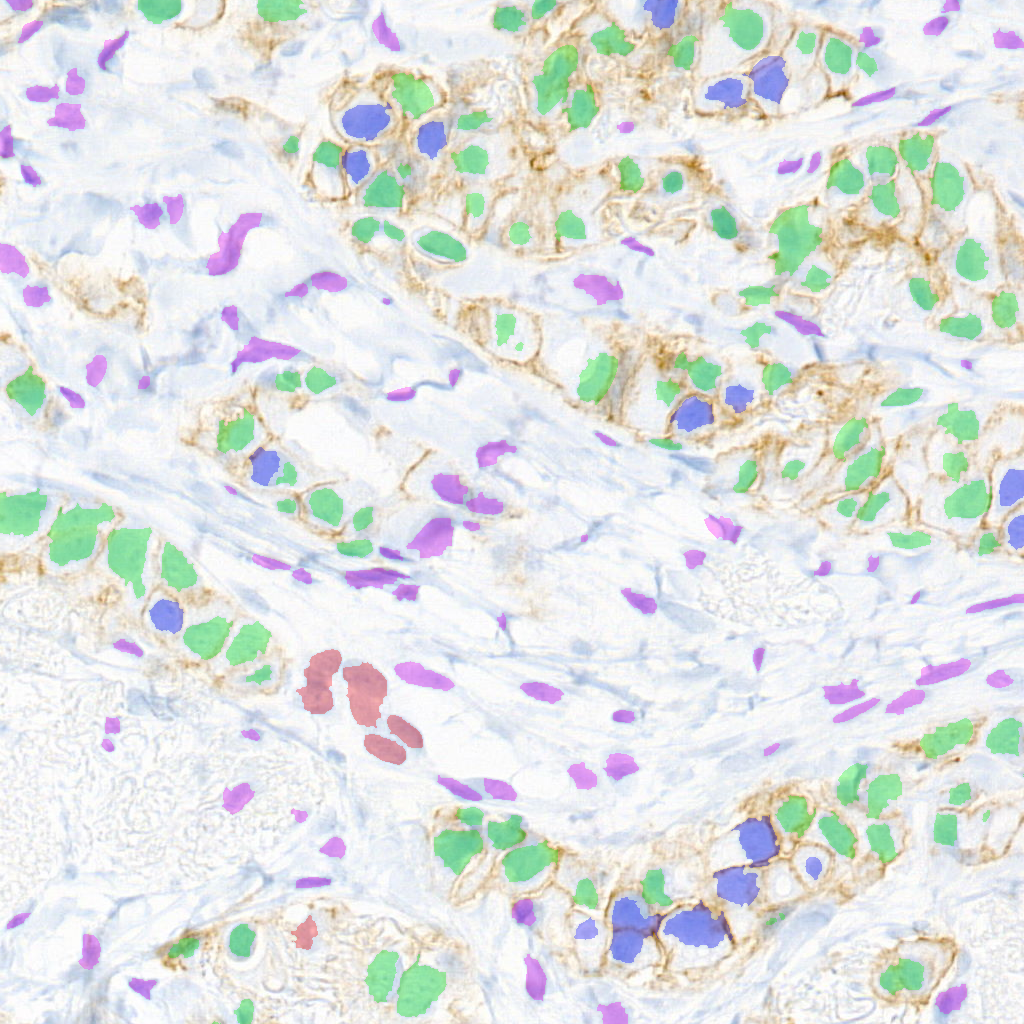
\includegraphics[width=\textwidth]{imgs/qual/breast/gt3.overlay.png}
    \label{fig:breast-gt3}
  \end{subfigure}
    \caption{Three examples with their ground truth overlayed on top.}
    \label{fig:breast-ex}
\end{figure}

That's right, the left one. It has clearly identifiable groups. The other two also have nests of cells but in between there are cells of other classes. In the first image the nests are clearly defined and separated between each others. Now comes the second question. Watch the next image in \autoref{fig:breast-hov1}, which is the output of Hovernet, and try to predict which are going to be the groups detected by the GCN trained with all the features, with probabilities only, with morphological features only and with features at all.

\begin{figure}[H]
    \centering
    \includegraphics[width=0.5\textwidth]{imgs/qual/breast/hov1.png}
    \caption{Output of Hovernet for the leftmost image of \autoref{fig:breast-ex}.}
    \label{fig:breast-hov1}
\end{figure}

This question was more tricky. Although GNNs behave predictably, there is still margin for uncertainty. The GCN with all the features has made the green cells eat their neighbours although it missed the group at top right which is detected by the model trained only with probabilities. On the other hand, the model that does not have Hovernet probabilities has predicted some red cells where the other predicted red or magenta. And the void model has played the safest of them all by just classifying everything with the dominant class. Note that being safe does not mean being good. It is just a poetic license to state that it did not bother trying to identify minority groups.

\begin{figure}[H]
  \centering
  \begin{subfigure}[b]{0.45\textwidth}
    \includegraphics[width=\textwidth]{imgs/qual/breast/gcn-full1.png}
    \caption{GT}
    \label{fig:breast-gt1}
  \end{subfigure}
  \hfill
  \begin{subfigure}[b]{0.45\textwidth}
    \includegraphics[width=\textwidth]{imgs/qual/breast/no-prior1.png}
    \caption{Morphological features}
    \label{fig:breast-no-prior1}
  \end{subfigure}
  \\
  \begin{subfigure}[b]{0.45\textwidth}
    \includegraphics[width=\textwidth]{imgs/qual/breast/no-morph1.png}
    \caption{Probabilities}
    \label{fig:breast-no-morph1}
  \end{subfigure}
  \hfill
  \begin{subfigure}[b]{0.45\textwidth}
    \includegraphics[width=\textwidth]{imgs/qual/breast/void1.png}
    \caption{Void}
    \label{fig:consep-void}
  \end{subfigure}
  \caption{Output of the GCN trained with different sets of input features.}
  \label{fig:breast-qual1}
\end{figure}

In \autoref{fig:breast-qual2} and \autoref{fig:breast-qual3} there are the outputs for the other two images from the beginning. Graph networks try to find clusters, sometimes they guess it right, sometimes they don't. Hovernet, as usual, tries to identify lonely cells correctly. Again, sometimes it works, sometimes it does not.


\begin{figure}[H]
  \centering
  \begin{subfigure}[b]{0.45\textwidth}
    \includegraphics[width=\textwidth]{imgs/qual/breast/gt2.overlay.png}
    \caption{GT}
    \label{fig:breast-gt2}
  \end{subfigure}
  \hfill
  \begin{subfigure}[b]{0.45\textwidth}
    \includegraphics[width=\textwidth]{imgs/qual/breast/hov2.png}
    \caption{Hovernet}
    \label{fig:breast-hov2}
  \end{subfigure}
  \\
  \begin{subfigure}[b]{0.45\textwidth}
    \includegraphics[width=\textwidth]{imgs/qual/breast/gcn-full2.png}
    \caption{GCN}
    \label{fig:breast-gcn2}
  \end{subfigure}
  \hfill
  \begin{subfigure}[b]{0.45\textwidth}
    \includegraphics[width=\textwidth]{imgs/qual/breast/no-morph2.png}
    \caption{Probabilities only}
    \label{fig:breast-no-morph2}
  \end{subfigure}
  \\
  \begin{subfigure}[b]{0.45\textwidth}
    \includegraphics[width=\textwidth]{imgs/qual/breast/no-prior2.png}
    \caption{Morphological features only}
    \label{fig:breast-no-prior2}
  \end{subfigure}
  \hfill
  \begin{subfigure}[b]{0.45\textwidth}
    \includegraphics[width=\textwidth]{imgs/qual/breast/void2.png}
    \caption{Void}
    \label{fig:breast-void2}
  \end{subfigure}
  \caption{Illustration of the behaviour of the different models.}
  \label{fig:breast-qual2}
\end{figure}


\begin{figure}[H]
  \centering
  \begin{subfigure}[b]{0.45\textwidth}
    \includegraphics[width=\textwidth]{imgs/qual/breast/gt3.overlay.png}
    \caption{GT}
    \label{fig:breast-gt3}
  \end{subfigure}
  \hfill
  \begin{subfigure}[b]{0.45\textwidth}
    \includegraphics[width=\textwidth]{imgs/qual/breast/hov3.png}
    \caption{Hovernet}
    \label{fig:breast-hov3}
  \end{subfigure}
  \\
  \begin{subfigure}[b]{0.45\textwidth}
    \includegraphics[width=\textwidth]{imgs/qual/breast/gcn-full3.png}
    \caption{GCN}
    \label{fig:breast-gcn3}
  \end{subfigure}
  \hfill
  \begin{subfigure}[b]{0.45\textwidth}
    \includegraphics[width=\textwidth]{imgs/qual/breast/no-morph3.png}
    \caption{Probabilities only}
    \label{fig:breast-no-morph3}
  \end{subfigure}
  \\
  \begin{subfigure}[b]{0.45\textwidth}
    \includegraphics[width=\textwidth]{imgs/qual/breast/no-prior3.png}
    \caption{Morphological features only}
    \label{fig:breast-no-prior3}
  \end{subfigure}
  \hfill
  \begin{subfigure}[b]{0.45\textwidth}
    \includegraphics[width=\textwidth]{imgs/qual/breast/void3.png}
    \caption{Void}
    \label{fig:breast-void3}
  \end{subfigure}
  \caption{Yet another illustration of the behaviour of the different models.}
  \label{fig:breast-qual3}
\end{figure}

To finish this section I will compare graph convolution to graph attention. Graph attention networks also create nests of cells. The difference now is that the attention network is trying to detect smaller groups and mixed groups. This may derive from the fact that the attention mechanism gives more flexibility in how labels are propagated through the graph. With the convolution everything gets spread equally likely. But with attention other patterns can emerge and, in fact, emerge. In \autoref{fig:breast-ex2} we can see that in the first pair the graph attention has surrounded a green group by a red group. That is quite unlikely for convolution to do. With the convolution cells get eaten by the biggest group. In the second pair there are some blue cells that are alone in the GAT case and more group diversity. If we consider graph networks to act as regularisers, then GCN penalizes more the existence of lonely cells than GAT.

\begin{figure}[H]
    \centering
    \begin{subfigure}[b]{0.45\textwidth}
    \includegraphics[width=\textwidth]{imgs/qual/breast/gcn-full1.png}
    \caption{GCN}
  \end{subfigure}
  \hfill
  \begin{subfigure}[b]{0.45\textwidth}
    \includegraphics[width=\textwidth]{imgs/qual/breast/gat-full1.png}
    \caption{GAT}
  \end{subfigure}
  \\
  \begin{subfigure}[b]{0.45\textwidth}
    \includegraphics[width=\textwidth]{imgs/qual/breast/gcn-full3.png}
    \caption{GCN}
  \end{subfigure}
  \hfill
  \begin{subfigure}[b]{0.45\textwidth}
    \includegraphics[width=\textwidth]{imgs/qual/breast/gat-full3.png}
    \caption{GAT}
  \end{subfigure}
    \caption{Comparison of graph convolution and graph attention predictions.}
    \label{fig:breast-ex2}
\end{figure}

\newpage
\subsection{DigiPatics lung}

I was personally involved in the creation of this dataset. This means that I know some information that is normally not documented in these databases. When labelling, the physician sometimes decided entirely based on information not present on the image itself. Or information present in the image but very subtle. One such case is the cilium. Cells near cilium are never tumoural but can be very similar to tumoural cells. In all the experiments we made, including those that are not documented here, the specific image in \autoref{fig:lung-cilium} was always predicted as tumoural. However, our best performing graph model somehow solved that problem. It is possible that it has been pure luck. But it is still remarkable because we didn't have such luck with Hovernet.

\begin{figure}[H]
    \centering
    \begin{subfigure}[b]{0.3\textwidth}
    \includegraphics[width=\textwidth]{imgs/qual/lung/cilio-gt.overlay.png}
    \caption{GT}
  \end{subfigure}
  \begin{subfigure}[b]{0.3\textwidth}
    \includegraphics[width=\textwidth]{imgs/qual/lung/cilio-hov.png}
    \caption{Hovernet}
  \end{subfigure}
  \begin{subfigure}[b]{0.3\textwidth}
    \includegraphics[width=\textwidth]{imgs/qual/lung/cilio-no-prior.png}
    \caption{GCN without probabilities}
  \end{subfigure}
    \caption{Example of an image containing cilium together with Hovernet and GNN predictions.}
    \label{fig:lung-cilium}
\end{figure}

Another special case is shown in \autoref{fig:lung-context}. When labelling this specific patch, Irene needed a few minutes to notice that it was not tumoural at all. And she discovered that by looking at the whole slide image. I was told that with that image alone it was not possible to be 100\% sure that all the cells were not tumoural. And we can see that both Hovernet and the GNN fail in this case. The cells marked in blue look so similar to tumoural cells that the models classify them as that because they lack the information needed to discard them from being tumoural.

\begin{figure}[H]
    \centering
    \begin{subfigure}[b]{0.3\textwidth}
    \includegraphics[width=\textwidth]{imgs/qual/lung/context-gt.overlay.png}
    \caption{GT}
  \end{subfigure}
  \begin{subfigure}[b]{0.3\textwidth}
    \includegraphics[width=\textwidth]{imgs/qual/lung/context-hov.png}
    \caption{Hovernet}
  \end{subfigure}
  \begin{subfigure}[b]{0.3\textwidth}
    \includegraphics[width=\textwidth]{imgs/qual/lung/context-no-prior.png}
    \caption{GCN without probabilities}
  \end{subfigure}
    \caption{Example of a patch that required extra context to label together with Hovernet and GNN predictions.}
    \label{fig:lung-context}
\end{figure}
\newpage
To finish this chapter I will leave a canonical example of when graphs are a good fit. The case depicted in \autoref{fig:lung-val} contains three groups perfectly separated from each other. Two nests of tumoural cells at both sides and in the middle a group of healthy cells. Hovernet struggles to detect some of the tumoural cells from the left and right. Probably because they are small, round and with a low nuclei to cytoplasm ratio, which are the properties typical of non-tumoural cells. But they are indeed tumoural, in part because they are all so close together. The graph network, on the other hand, leverages the fact that they are grouped together and propagates the dominant class of each cluster to all the cells of that cluster, perfectly classifying the whole patch.

\begin{figure}[H]
    \centering
    \begin{subfigure}[b]{0.3\textwidth}
    \includegraphics[width=\textwidth]{imgs/qual/lung/val-gt1.overlay.png}
    \caption{GT}
  \end{subfigure}
  \begin{subfigure}[b]{0.3\textwidth}
    \includegraphics[width=\textwidth]{imgs/qual/lung/val-hov1.png}
    \caption{Hovernet}
  \end{subfigure}
  \begin{subfigure}[b]{0.3\textwidth}
    \includegraphics[width=\textwidth]{imgs/qual/lung/val-no-prior1.png}
    \caption{GCN without probabilities}
  \end{subfigure}
    \caption{Another example from the validation dataset where the graph network is clearly better than Hovernet.}
    \label{fig:lung-val}
\end{figure}


\chapter{Conclusions}

Digital pathology can be very difficult to tackle. Our experiments have showed that there is not a single method that works properly in every setup. Each organ and stain requires their own specific and carefully designed model. For lung and H\&E stain the method proposed not only works better than previous state of the art models but our experiments have proven that it is properly leveraging extra information hidden to computer vision algorithms and tabular methods like XGBoost. Domain expertise was key for designing the algorithm. By talking to real experts on the topic I was able to discover how important the neighbourhood of a cell was to classify it as tumoural or not. Since in digital pathology data is so scarce, discovering such inductive biases can be very valuable. A simple vision transformer would easily solve this problem with billions of images. But we have hundreds. That is why the method presented in this thesis is so valuable, because of its sample efficiency.
\chapter{Future work}

The obvious lines of research here are improving the CNN backbone, improving the GNN head or training everything end-to-end instead of having two-phases as in this work. All of them would bring better metrics and more robust classification methods. However, the obvious is not always the best. Progress is made by impressive discoveries that few people expected. That is why I want to propose a different way of advancing science in this field. The classification paradigm has served us well, but a new paradigm is emerging nowadays. Multimodal models are on the rise. Image captioning models like BLIP \cite{li2022blip} or CLIP \cite{radford2021learning} have gained popularity in the last years. They provide a way of opening the black boxes that are neural networks. Captioning an image is just one step behind a model explaining itself and the reasoning about the result. Why not make a model explain cancer? Expert pathologist train new physicians showing them images and explaining them with voice or text. Why not train models the same way? Obviously those models won't be better than the experts, but they can outscale them. One person can only view a small amount of patients in a life. A model can be trained with billions of cases in months and can infer the result of millions of new cases in days given enough computational resources. So that is the non-obvious future work: Image captioning for medical image analysis.

I'll use the rest of the page to describe the roadmap to achieving the goal of medical images explaining themselves. First step: data. That is the most important part of the whole project. No data no models. Typically foundational models require billions of image-text pairs, or if only trained with text they require trillions of tokens. Such amount of medical data is not available yet, although it would be possible if experts were into it. But I'll assume physicians don't really want to spend time creating datasets (which is more or less my experience dealing with doctors). The good news is that one can fine-tune a foundational model with smaller amounts of data. With thousands of image-text pairs would be enough for a production ready model. To obtain such pairs pathologist would be required to think loud. That's it. We can automatically transcribe audio into text, so it is enough for them to record their voice while working. The next step is the model. In the previous paragraph I have shown two methods of jointly training a latent text-image space. But we can achieve much more than that, we want to speak to the images. Something like what is done in Mini-GPT4 \cite{zhu2023minigpt4}. Right now there is a wide variety of language models to be used as backbones. Stability AI recently released StableLM\footnote{\url{https://github.com/Stability-AI/StableLM}}, and we have the LLaMa family of models too\footnote{\url{https://ai.facebook.com/blog/large-language-model-llama-meta-ai/}}. We are not running out of open source LLMs anytime soon. Using them is a huge boost in performance and sample efficiency. Moreover, there is also DINOv2\footnote{\url{https://dinov2.metademolab.com/}} which can be used as image encoder to further reduce the burden of training. We just need to merge everything and finetune it with the appropiate data. Sounds easy, right?
\printbibliography[heading=bibintoc]
\appendix
\chapter{Sustainability and costs}

This project was carried out by a single student, which means the cost of it was very low. However, a project that depends on students is not a sustainable one since students are highly underpaid. For that reason I would like to provide a quantitative analysis on the real costs of carrying out this work. 

Let's start counting the hours of work required to just build the dataset. Even after using a semi-automatic procedure to label the data, many hours were needed to end up with 85 labelled images. Roughly 100 hours of human labour and 20 hours of compute power were employed to create segmentations. Another 15 hours of expert human labour were required to review the class annotations by the physician. Now, let's translate that into money. The first 100 hours required very low training, just the ability to paint circles. A fair salary for that can be 10€/h (if outsourced it could be less than 2€/h). That translates into a cost of 1000€. The compute power requires GPUs that consume at most 350W. Let's estimate the CPU, memory and GPU consumption by 300W on average, which means $4.5$kWh were consumed. That means $0.93$€ if the price of electricity is $0.15$€/kWh. And the expert work is typically paid more, let's estimate 20€/h which means 300€ in total. The total cost of creating the database would be $1300.93$€. If we divide by the number of images we have a total of $15.30$€ per image. 

Second, the salary of the technical workers. A project like this normally requires a software developer, a data engineer and a project manager. Depending on the experience the salaries may range. For simplicity, let's consider the software developer is junior (30K/year), the data engineer is senior (50K/year) and the project manager has nearly five years of experience (80K/year). Assuming the project is carried out in just one year, and taking into account the extra 30\% that needs to be payed to the social security, the total cost in salaries would be $208000$€.

Third, putting a machine learning model in production is more than just creating it. It needs to be maintained, and someone has to care about the drift. Models performs worse when time passes because the data distribution is not fixed. New patients means new training is needed. Hospitals would need to train their technicians to perform retrainings and physicians to relabel. The cost of relabelling is already estimated: $15.30$€ per image. Remains to estimate the cost of training technicians. 385\$ or 350€ per person is what a course on machine learning would cost\footnote{\url{https://www.ml.school/c/start-here} Accessed 8th April 2023}.

Finally, to show that the project is sustainable, it has to generate some value. I believe in open science and medicine. Putting a price in other people's lives is not ethical, so privatising this project is not an option. But someone has to pay the cost, in this case, the government. A project like this is only sustainable if public opinion is in favour of it. More data is needed to exactly estimate the social value this will bring. In my opinion, this product will reduce physician workloads, which is beneficial. By reducing the workload, the diagnostic process can be accelerated, and receiving faster diagnostics is something the public opinion will definitely be interested about.

\chapter{The problem of merging cells}\label{sec:merge_cells}

One of the problems that appeared when using Hovernet was broken cells. In many cases, big cells were predicted as various small cells. It is visually appalling and that is why we designed an algorithm to merge broken cells. The result is on \autoref{fig:morph_}.

\begin{figure}[ht]
\begin{subfigure}[b]{1\textwidth}
    \centering
    \includegraphics[width=\textwidth]{imgs/morph1.png}
    \caption{Before}
    \label{fig:morph1}
\end{subfigure}
\begin{subfigure}[b]{1\textwidth}
    \centering
    \includegraphics[width=\textwidth]{imgs/morph2.png}
    \caption{After}
    \label{fig:morph2}
\end{subfigure}
\caption{Example of cells that were not fully detected by Hovernet. After applying our algorithm all the smaller cells were merged into one.}
\label{fig:morph_}
\end{figure}

The algorithm leverages techniques of mathematical morphology. If we call $X_1$ the predicted image and $X_2$ the image that identifies the background with the value zero and the rest with one, then, the image $(\delta (X_1) - X_1)  \cdot X_2$ contains the frontiers of the cells, being $\delta$ a dilation. An illustration of the process is on \autoref{fig:morph}.

\begin{figure}[ht]
    \centering
    \includegraphics[width=0.5\textwidth]{imgs/morphInflam.png}
    \caption{Top-left is the original image, top-right is the dilation, bottom-left the gradient and bottom-right the masking which is the final result.}
    \label{fig:morph}
\end{figure}

The problem here is that different frontiers may end up with the same identifier. $X_1$ contains the identifier of each cell in every pixel of such cell. But, $(\delta (X_1) - X_1)  \cdot X_2$ contains the differences of identifiers in the position of the frontier. Differences of different pairs may end up with the same value. E.g.: $4-3 = 2-1$. To solve that, it is needed to properly set the identifiers so that each pair can be uniquely identified by the difference between the maximum and the minimum. One simple solution to that is to use powers of two. More concretely, applying the function $n \mapsto 2^n$ to the identifiers. This way $2^n-2^m$ is a function that can be inverted back to the pair $(n,m)$ where $n>m$. However, we can have up to 1500 cells, requiring identifiers up to $2^{1500}$ is clearly unfeasible and is not computationally optimal since to identify pairs we only need $1500 \choose 2$ $=1.124.250$ identifiers. The best function I have found so far is $n \mapsto n^5$, using other simple lower degree polynomials doesn't uniquely identify the difference for values up to 1500 \cite{4567383}.

\chapter{TumourKit}

The whole thesis dealt with the theory and the results of the experiments. Behind all that there was a lot of software needed to make it all work. I decided to build a python library that other people could use to replicate my experiments and design new ones. The library is called TumourKit. The code is available on GitHub\footnote{\url{https://github.com/Jerry-Master/lung-tumour-study}} under the Affero GPLv3 license. It is tested on Ubuntu and Windows for python versions 3.8, 3.9 and 3.10. It has more than ten thousands lines of code, counting comments. For a more detailed explanation on how to use it and what is offered, please, read the docs\footnote{\url{https://lung-tumour-study.readthedocs.io/en/latest/}}.

\chapter{Soft Labels}

One of the problems we encountered when reviewing the lung dataset was that the expert was not sure which label to give to some cells. It was solved by simply ignoring those cells since in practice it didn't really matter because we are interested in percentages and a cell with no label can be removed from the numerator and denominator. However, we do preserve that information in the dataset because it could be used to train the models with soft labels. Even though we didn't try it, we expect it could help further calibrate the resulting probabilities. For that reason, in this appendix I will be explaining how to adapt all the methods presented in the thesis to soft labels. 

The easiest ones to adapt are the graph neural networks. They are trained using the softmax, so they are already compatible with soft labels. It is only needed to substitute the one hot encoded vector of labels to a vector of probabilities and everything works exactly the same.

The XGBoost method requires a little trick. Although XGBoost also uses softmax for training, current implementations threshold the label so providing probabilities is of no use since the soft labels will be made into hard labels. Nonetheless, XGBoost supports a weight for each row in the dataset. This makes it possible to use the probabilities as weights. The trick consists of repeating rows one time for each class and assign that class probability to that repeated row weight. The idea was taken for an online forum\footnote{\url{https://stackoverflow.com/a/66481600}} and the explanation behind how this works is that XGBoost multiplies the gradient and hessian by the weight and not by the label, as explained in another online forum\footnote{\url{https://stats.stackexchange.com/a/365555/378093}}. 

The trickiest method to adapt is HoVerNet. Having soft labels does not affect neither the HV branch nor the NP branch but it does affect the NC branch. That branch is trained using the softmax and the dice loss. The first one is quite easy to adapt as described for the graph neural networks. However, the dice loss requires more thinking. In Zifu Wang et al. \cite{wang2023dice} they propose a way of extending the dice loss for soft labels with promising results. On a more technical and practical level, modifying the codebase to support this metric is too much of a hurdle given the expected benefits. But it is interesting on a theoretical perspective to know of the existence of such possibility. In the future, when it becomes a more refined technique with wider support on the main libraries, it may be a good way of training better models.

\chapter{Hyperparameter study}\label{chap:hyper}

Instead of showing the losses here which would be pretty useless since there are 32 configurations per dataset and for each configuration we track 5 or 6 metrics. That much information cannot be shown in a non-interactive way. Therefore, we provide public links to the tensorboard logs with all the training and validation metrics for every configuration. This way you can see how every configuration evolved in time and filter by hyperparameters. The naming convention is as follows. The first letters are either GCN or ATT meaning graph convolution of attention. Then, the next number is the number of layer, after that is the dropout value and then whether or not it used batch normalisation. So, ATT\_10\_0.3\_bn means graph attention with 10 layers and 30\% of dropout with batch normalisation. The links are below, if you do not see anything it may be because you need to select some configurations in the left bar.

\begin{itemize}
    \item DigiPatics lung: \url{https://tensorboard.dev/experiment/HVSvkl8LQyuNWIWw4dgNmg/} 
    \item DigiPatics breast: \url{https://tensorboard.dev/experiment/cQoaRA5GRZSEdYh3ijuPmw/}
    \item CoNSeP: \url{https://tensorboard.dev/experiment/Zb6YbBWWSO6q17DdMEVtZw/}
    \item MoNuSAC: \url{https://tensorboard.dev/experiment/rfvi7c48Q7CEU7yNvdxEGg/}
\end{itemize}

I am also providing links to the tensorboard logs of every void gnn experiment. For DigiPatics lung:

\begin{itemize}
    \item Probabilities: \url{https://tensorboard.dev/experiment/3Q9pt4KlSvWiv6xAeEE3cA/}
    \item Morphological: \url{https://tensorboard.dev/experiment/hgMqRfVbRr2XWs0xKmX2sQ/}
    \item Void: \url{https://tensorboard.dev/experiment/Ko52fAFqTRyKXwqXRQx4gQ/}
\end{itemize}

\noindent For DigiPatics breast:

\begin{itemize}
    \item Probabilities: \url{https://tensorboard.dev/experiment/tVB2jfeWR4yWuolpKaEBFg/}
    \item Morphological: \url{https://tensorboard.dev/experiment/o1QXFlsMSPGo6zmVNY7f1g/}
    \item Void: \url{https://tensorboard.dev/experiment/IMC4U8y9R7KXzwaJMlm2Qg/}
\end{itemize}

\noindent For CoNSeP:

\begin{itemize}
    \item Probabilities: \url{https://tensorboard.dev/experiment/uRu2tXp0Rr6HKVJ7bend0w/}
    \item Morphological: \url{https://tensorboard.dev/experiment/tBlaEjlqRJyTq5NfMGMWEg/}
    \item Void: \url{https://tensorboard.dev/experiment/aKsWfarRTYmw1CGyZY37RA/}
\end{itemize}

\noindent For MoNuSAC:

\begin{itemize}
    \item Probabilities: \url{https://tensorboard.dev/experiment/EPvvFnj1SGC5AgE7geJmRA/}
    \item Morphological: \url{https://tensorboard.dev/experiment/gS9WVXkHQTapbAZNT2lOjQ/}
    \item Void: \url{https://tensorboard.dev/experiment/e6lLbjeZRwCO4Avz2Ar03A/}
\end{itemize}

\noindent The best configuration of hyperparameters for each dataset can be found on \autoref{tab:E} and the test metrics of every configuration are presented in the remaining tables of this appendix. Keep in mind that these metrics are on the test set and provided only for curious readers. They were never used in the selection of the model nor configuration since we only used the validation set for that. In fact, you can see that the best metrics here are not always the same as the metrics presented. Also for curious readers, more tensorboard links are provided from the training of Hovernet below. Tensorboard dev does not support image visualisation so, even though I have image logs they cannot be shared easily. If you are interested on them, feel free to email me for it. Here, 00 is the first phase of the training where the encoder was frozen and 01 is the second phase of training which was done after 00 and had the encoder unfrozen.

\begin{itemize}
    \item DigiPatics lung: \url{https://tensorboard.dev/experiment/Ah3wt2t9Tl6ArIQ1qqGXDQ/}
    \item DigiPatics breast: \url{https://tensorboard.dev/experiment/W416onQiQbaAkWpplkm4TA/}
    \item CoNSeP: \url{https://tensorboard.dev/experiment/vcz3QWa2SouqvqYOGpVpXg/}
    \item MoNuSAC: \url{https://tensorboard.dev/experiment/3g6kp9xmTa6a6jKcxUAJcw/}
\end{itemize}

The main takeaway from all this information is that there is no golden rule. Do not try to find any pattern, there is not any. Sometimes more layers is better, sometimes is not. Sometimes dropout works sometimes it does not. You always need to optimise for those hyperparameters since every problem is different and no intuition can be obtained from empirical data about the behaviour of those hyperparameters. If you want better results you are forced to use more compute power.

\begin{table}[ht]
    \centering
    \caption{Best hyperparameter configurations.}
    \begin{tabular}{|c|c|c|c|}
    \hline
    Dataset & \#Layers & Dropout & Batch Normalisation\\ \hline
       DigiPatics lung  & 5 & 0.9 & Yes \\ \hline
       DigiPatics breast  & 1 & 0.6 & Yes \\ \hline
       CoNSeP  & 1 & 0.0 & Yes \\ \hline
       MoNuSAC  & 15 & 0.3 & No \\ \hline
    \end{tabular}
    \label{tab:E}
\end{table}

\begin{table}[ht]
    \centering
    \caption{Graph convolution hyperparameter optimization on DigiPatics lung.}
\begin{tabular}{|c|c|c|c|c|c|c|c|}
\hline
F1 & Acc & AUC & \%ERR & ECE & \#Layers & Dropout & Norm type\\ \hline
62.77\% & 82.67\% & 84.94\% & 6.96\% & 0.0711 & 1 & 0.0 & bn\\ \hline
69.44\% & 83.53\% & 90.06\% & 0.38\% & 0.0646 & 1 & 0.0 & None\\ \hline
61.95\% & 82.55\% & 87.01\% & 7.64\% & 0.0761 & 1 & 0.3 & bn\\ \hline
68.54\% & 84.13\% & \textbf{90.44\%} & 3.06\% & \textbf{0.0415} & 1 & 0.3 & None\\ \hline
63.00\% & 82.63\% & 88.05\% & 6.56\% & 0.0810 & 1 & 0.6 & bn\\ \hline
68.04\% & 83.23\% & 89.97\% & 1.04\% & 0.0593 & 1 & 0.6 & None\\ \hline
65.46\% & 83.15\% & 88.41\% & 4.72\% & 0.0544 & 1 & 0.9 & bn\\ \hline
66.94\% & 83.75\% & 89.89\% & 4.36\% & 0.0504 & 1 & 0.9 & None\\ \hline
62.83\% & 82.67\% & 86.84\% & 6.88\% & 0.0601 & 5 & 0.0 & bn\\ \hline
64.78\% & 83.03\% & 87.29\% & 5.32\% & 0.0902 & 5 & 0.0 & None\\ \hline
62.87\% & 82.63\% & 83.14\% & 6.72\% & 0.0746 & 5 & 0.3 & bn\\ \hline
64.21\% & 83.09\% & 87.43\% & 6.26\% & 0.0870 & 5 & 0.3 & None\\ \hline
63.74\% & 82.97\% & 85.23\% & 6.54\% & 0.0622 & 5 & 0.6 & bn\\ \hline
64.87\% & 83.33\% & 87.56\% & 6.06\% & 0.0951 & 5 & 0.6 & None\\ \hline
66.53\% & 83.27\% & 86.84\% & 3.52\% & 0.0884 & 5 & 0.9 & bn\\ \hline
66.43\% & 83.29\% & 88.50\% & 3.74\% & 0.1117 & 5 & 0.9 & None\\ \hline
56.93\% & 81.59\% & 86.89\% & 10.77\% & 0.0596 & 10 & 0.0 & bn\\ \hline
66.75\% & 83.63\% & 87.10\% & 4.28\% & 0.0873 & 10 & 0.0 & None\\ \hline
63.77\% & 82.81\% & 85.40\% & 6.06\% & 0.0451 & 10 & 0.3 & bn\\ \hline
67.15\% & 83.67\% & 86.78\% & 3.80\% & 0.0907 & 10 & 0.3 & None\\ \hline
66.48\% & 83.31\% & 86.34\% & 3.72\% & 0.0828 & 10 & 0.6 & bn\\ \hline
65.55\% & 83.13\% & 86.28\% & 4.54\% & 0.0924 & 10 & 0.6 & None\\ \hline
65.73\% & 83.35\% & 86.69\% & 4.92\% & 0.0846 & 10 & 0.9 & bn\\ \hline
71.42\% & 84.27\% & 86.95\% & 1.52\% & 0.1190 & 10 & 0.9 & None\\ \hline
66.06\% & 83.71\% & 89.08\% & 5.52\% & 0.0439 & 15 & 0.0 & bn\\ \hline
71.31\% & 84.57\% & 86.82\% & \textbf{0.26\%} & 0.0663 & 15 & 0.0 & None\\ \hline
57.77\% & 81.83\% & 81.31\% & 10.49\% & 0.0563 & 15 & 0.3 & bn\\ \hline
69.03\% & 84.27\% & 86.83\% & 2.72\% & 0.0612 & 15 & 0.3 & None\\ \hline
67.36\% & 83.07\% & 85.58\% & 1.64\% & 0.0686 & 15 & 0.6 & bn\\ \hline
68.74\% & 83.87\% & 86.79\% & 1.92\% & 0.0972 & 15 & 0.6 & None\\ \hline
70.74\% & \textbf{84.75\%} & 86.89\% & 1.40\% & 0.0842 & 15 & 0.9 & bn\\ \hline
\textbf{73.50\%} & 84.59\% & 87.66\% & 4.64\% & 0.1351 & 15 & 0.9 & None\\ \hline
\end{tabular}
\end{table}

\begin{table}[ht]
    \centering
    \caption{Graph attention hyperparameter optimization on DigiPatics lung.}
\begin{tabular}{|c|c|c|c|c|c|c|c|}
\hline
F1 & Acc & AUC & \%ERR & ECE & \#Layers & Dropout & Norm type\\ \hline
56.81\% & 81.59\% & 84.26\% & 10.89\% & 0.0356 & 1 & 0.0 & bn\\ \hline
61.03\% & 82.37\% & 90.23\% & 8.26\% & 0.0910 & 1 & 0.0 & None\\ \hline
60.63\% & 82.43\% & 86.74\% & 8.89\% & 0.0795 & 1 & 0.3 & bn\\ \hline
55.89\% & 81.49\% & 89.34\% & 11.55\% & 0.0982 & 1 & 0.3 & None\\ \hline
64.28\% & 83.03\% & 88.51\% & 6.00\% & 0.1065 & 1 & 0.6 & bn\\ \hline
65.02\% & 83.03\% & 89.35\% & 5.00\% & 0.0817 & 1 & 0.6 & None\\ \hline
3.67\% & 73.74\% & 88.90\% & 26.26\% & 0.1446 & 1 & 0.9 & bn\\ \hline
41.83\% & 78.63\% & 86.76\% & 16.77\% & 0.1009 & 1 & 0.9 & None\\ \hline
59.73\% & 82.11\% & 85.68\% & 9.09\% & 0.0548 & 5 & 0.0 & bn\\ \hline
63.85\% & 82.87\% & 87.43\% & 6.12\% & 0.1014 & 5 & 0.0 & None\\ \hline
47.42\% & 80.25\% & 87.61\% & 15.95\% & 0.1143 & 5 & 0.3 & bn\\ \hline
67.32\% & 83.97\% & 87.78\% & 4.46\% & 0.1376 & 5 & 0.3 & None\\ \hline
67.84\% & 84.29\% & \textbf{91.34\%} & 4.66\% & 0.1086 & 5 & 0.6 & bn\\ \hline
68.88\% & 83.71\% & 89.21\% & 1.16\% & 0.1233 & 5 & 0.6 & None\\ \hline
0.00\% & 73.24\% & 76.25\% & 26.76\% & \textbf{0.0171} & 5 & 0.9 & bn\\ \hline
0.00\% & 73.24\% & 39.62\% & 26.76\% & 0.2574 & 5 & 0.9 & None\\ \hline
53.42\% & 80.95\% & 89.55\% & 12.61\% & 0.1048 & 10 & 0.0 & bn\\ \hline
55.01\% & 81.77\% & 86.10\% & 12.99\% & 0.1321 & 10 & 0.0 & None\\ \hline
68.69\% & 84.09\% & 89.74\% & 2.70\% & 0.0499 & 10 & 0.3 & bn\\ \hline
67.44\% & 83.63\% & 90.76\% & 3.24\% & 0.0791 & 10 & 0.3 & None\\ \hline
0.00\% & 73.24\% & 89.37\% & 26.76\% & 0.0914 & 10 & 0.6 & bn\\ \hline
0.00\% & 73.24\% & 31.83\% & 26.76\% & 0.2673 & 10 & 0.6 & None\\ \hline
0.00\% & 73.24\% & 50.00\% & 26.76\% & 0.1027 & 10 & 0.9 & bn\\ \hline
0.00\% & 73.24\% & 37.30\% & 26.76\% & 0.2674 & 10 & 0.9 & None\\ \hline
71.79\% & 84.57\% & 89.85\% & 1.18\% & 0.0526 & 15 & 0.0 & bn\\ \hline
71.71\% & \textbf{84.87\%} & 89.95\% & \textbf{0.04\%} & 0.0863 & 15 & 0.0 & None\\ \hline
67.23\% & 84.51\% & 89.59\% & 6.24\% & 0.0727 & 15 & 0.3 & bn\\ \hline
\textbf{73.56\%} & 84.69\% & 89.90\% & 4.38\% & 0.0750 & 15 & 0.3 & None\\ \hline
0.00\% & 73.24\% & 75.87\% & 26.76\% & 0.0691 & 15 & 0.6 & bn\\ \hline
11.18\% & 60.58\% & 39.72\% & 9.13\% & 0.2755 & 15 & 0.6 & None\\ \hline
0.00\% & 73.24\% & 54.20\% & 26.76\% & 0.0490 & 15 & 0.9 & bn\\ \hline
0.00\% & 73.24\% & 22.17\% & 26.76\% & 0.2676 & 15 & 0.9 & None\\ \hline
\end{tabular}
\end{table}

\begin{table}[ht]
    \centering
    \caption{Graph convolution hyperparameter optimization on DigiPatics breast.}
\begin{tabular}{|c|c|c|c|c|c|c|}
\hline
Micro F1 & Macro F1 & Weighted F1 & ECE & \#Layers & Dropout & Norm type\\ \hline
70.56\% & 41.00\% & 70.63\% & 0.2542 & 1 & 0.0 & bn\\ \hline
68.57\% & 41.16\% & 68.07\% & 0.2712 & 1 & 0.0 & None\\ \hline
68.84\% & 40.92\% & 68.72\% & 0.2674 & 1 & 0.3 & bn\\ \hline
\textbf{70.62\%} & 42.32\% & 70.52\% & 0.2565 & 1 & 0.3 & None\\ \hline
70.47\% & 42.53\% & 71.13\% & 0.2501 & 1 & 0.6 & bn\\ \hline
70.61\% & \textbf{42.81\%} & \textbf{71.87\%} & 0.2694 & 1 & 0.6 & None\\ \hline
69.35\% & 41.50\% & 69.37\% & 0.2587 & 1 & 0.9 & bn\\ \hline
70.04\% & 42.26\% & 70.13\% & 0.2571 & 1 & 0.9 & None\\ \hline
61.34\% & 41.90\% & 59.75\% & 0.2816 & 5 & 0.0 & bn\\ \hline
61.94\% & 41.87\% & 60.57\% & 0.2891 & 5 & 0.0 & None\\ \hline
55.93\% & 34.51\% & 54.45\% & 0.3007 & 5 & 0.3 & bn\\ \hline
55.42\% & 37.74\% & 53.37\% & 0.3143 & 5 & 0.3 & None\\ \hline
62.31\% & 42.61\% & 62.76\% & 0.2798 & 5 & 0.6 & bn\\ \hline
53.93\% & 34.59\% & 52.27\% & 0.3183 & 5 & 0.6 & None\\ \hline
69.40\% & 34.25\% & 67.53\% & \textbf{0.2423} & 5 & 0.9 & bn\\ \hline
61.47\% & 42.49\% & 61.90\% & 0.2881 & 5 & 0.9 & None\\ \hline
51.30\% & 29.90\% & 46.98\% & 0.3230 & 10 & 0.0 & bn\\ \hline
54.86\% & 34.87\% & 53.42\% & 0.3051 & 10 & 0.0 & None\\ \hline
51.57\% & 35.26\% & 50.82\% & 0.3037 & 10 & 0.3 & bn\\ \hline
55.64\% & 34.09\% & 54.02\% & 0.3004 & 10 & 0.3 & None\\ \hline
56.13\% & 37.90\% & 56.80\% & 0.2877 & 10 & 0.6 & bn\\ \hline
53.83\% & 32.87\% & 53.88\% & 0.3157 & 10 & 0.6 & None\\ \hline
65.87\% & 35.59\% & 62.88\% & 0.2681 & 10 & 0.9 & bn\\ \hline
65.58\% & 35.72\% & 62.66\% & 0.2938 & 10 & 0.9 & None\\ \hline
54.70\% & 36.89\% & 52.84\% & 0.2831 & 15 & 0.0 & bn\\ \hline
49.67\% & 31.46\% & 47.47\% & 0.3174 & 15 & 0.0 & None\\ \hline
57.22\% & 36.64\% & 55.77\% & 0.2797 & 15 & 0.3 & bn\\ \hline
54.38\% & 33.52\% & 54.51\% & 0.3062 & 15 & 0.3 & None\\ \hline
49.15\% & 29.97\% & 46.72\% & 0.3226 & 15 & 0.6 & bn\\ \hline
51.00\% & 31.14\% & 50.70\% & 0.3064 & 15 & 0.6 & None\\ \hline
64.98\% & 34.08\% & 61.82\% & 0.2581 & 15 & 0.9 & bn\\ \hline
64.20\% & 33.50\% & 60.95\% & 0.3143 & 15 & 0.9 & None\\ \hline
\end{tabular}
\end{table}

\begin{table}[ht]
    \centering
    \caption{Graph attention hyperparameter optimization on DigiPatics breast.}
\begin{tabular}{|c|c|c|c|c|c|c|}
\hline
Micro F1 & Macro F1 & Weighted F1 & ECE & \#Layers & Dropout & Norm type\\ \hline
64.57\% & 38.40\% & 65.43\% & 0.2772 & 1 & 0.0 & bn\\ \hline
61.67\% & 36.83\% & 60.40\% & 0.2867 & 1 & 0.0 & None\\ \hline
71.38\% & 40.58\% & 70.53\% & 0.2536 & 1 & 0.3 & bn\\ \hline
64.72\% & 38.37\% & 64.66\% & 0.2740 & 1 & 0.3 & None\\ \hline
69.49\% & \textbf{41.55\%} & 70.46\% & 0.2751 & 1 & 0.6 & bn\\ \hline
70.59\% & 41.34\% & 70.82\% & 0.2574 & 1 & 0.6 & None\\ \hline
44.75\% & 24.36\% & 31.87\% & 0.3307 & 1 & 0.9 & bn\\ \hline
\textbf{72.16\%} & 39.09\% & \textbf{71.57\%} & 0.2428 & 1 & 0.9 & None\\ \hline
52.85\% & 38.19\% & 49.38\% & 0.3166 & 5 & 0.0 & bn\\ \hline
55.56\% & 34.86\% & 52.16\% & 0.3158 & 5 & 0.0 & None\\ \hline
64.40\% & 37.01\% & 64.90\% & 0.2472 & 5 & 0.3 & bn\\ \hline
60.73\% & 38.45\% & 60.38\% & 0.2901 & 5 & 0.3 & None\\ \hline
66.05\% & 32.22\% & 63.85\% & 0.2583 & 5 & 0.6 & bn\\ \hline
59.78\% & 38.04\% & 55.77\% & 0.3445 & 5 & 0.6 & None\\ \hline
42.08\% & 14.81\% & 24.92\% & 0.2713 & 5 & 0.9 & bn\\ \hline
41.92\% & 14.77\% & 24.86\% & 0.3512 & 5 & 0.9 & None\\ \hline
40.25\% & 18.55\% & 32.70\% & 0.3634 & 10 & 0.0 & bn\\ \hline
46.88\% & 30.67\% & 44.74\% & 0.3398 & 10 & 0.0 & None\\ \hline
50.99\% & 27.44\% & 52.42\% & 0.3007 & 10 & 0.3 & bn\\ \hline
24.88\% & 22.21\% & 33.39\% & 0.4510 & 10 & 0.3 & None\\ \hline
42.08\% & 14.81\% & 24.92\% & 0.2850 & 10 & 0.6 & bn\\ \hline
48.18\% & 18.78\% & 35.70\% & 0.3670 & 10 & 0.6 & None\\ \hline
42.08\% & 14.81\% & 24.92\% & 0.2588 & 10 & 0.9 & bn\\ \hline
6.60\% & 3.09\% & 0.82\% & 0.5596 & 10 & 0.9 & None\\ \hline
43.95\% & 28.14\% & 46.56\% & 0.3415 & 15 & 0.0 & bn\\ \hline
45.56\% & 26.04\% & 41.67\% & 0.3567 & 15 & 0.0 & None\\ \hline
58.08\% & 27.71\% & 55.01\% & 0.3047 & 15 & 0.3 & bn\\ \hline
2.61\% & 1.96\% & 4.77\% & \textbf{0.2060} & 15 & 0.3 & None\\ \hline
42.08\% & 14.81\% & 24.92\% & 0.2838 & 15 & 0.6 & bn\\ \hline
25.31\% & 11.16\% & 23.68\% & 0.2399 & 15 & 0.6 & None\\ \hline
42.08\% & 14.81\% & 24.92\% & 0.2670 & 15 & 0.9 & bn\\ \hline
47.19\% & 19.39\% & 43.47\% & 0.2700 & 15 & 0.9 & None\\ \hline
\end{tabular}
\end{table}

\begin{table}[ht]
    \centering
    \caption{Graph convolution hyperparameter optimization on CoNSeP.}
\begin{tabular}{|c|c|c|c|c|c|c|}
\hline
Micro F1 & Macro F1 & Weighted F1 & ECE & \#Layers & Dropout & Norm type\\ \hline
64.31\% & 46.71\% & 61.36\% & 0.0530 & 1 & 0.0 & bn\\ \hline
63.67\% & 45.25\% & 60.02\% & 0.0419 & 1 & 0.0 & None\\ \hline
64.17\% & 47.01\% & 61.46\% & 0.0541 & 1 & 0.3 & bn\\ \hline
63.75\% & 46.39\% & 60.78\% & 0.0394 & 1 & 0.3 & None\\ \hline
61.74\% & 46.78\% & 59.18\% & 0.0637 & 1 & 0.6 & bn\\ \hline
\textbf{64.67\%} & \textbf{48.24\%} & \textbf{61.82\%} & 0.0415 & 1 & 0.6 & None\\ \hline
57.46\% & 26.66\% & 51.03\% & 0.0681 & 1 & 0.9 & bn\\ \hline
58.98\% & 26.46\% & 52.75\% & \textbf{0.0376} & 1 & 0.9 & None\\ \hline
62.66\% & 42.05\% & 59.30\% & 0.0544 & 5 & 0.0 & bn\\ \hline
58.77\% & 39.85\% & 56.42\% & 0.0589 & 5 & 0.0 & None\\ \hline
58.08\% & 32.41\% & 51.75\% & 0.0759 & 5 & 0.3 & bn\\ \hline
64.01\% & 46.02\% & 60.56\% & 0.0654 & 5 & 0.3 & None\\ \hline
46.21\% & 18.21\% & 34.93\% & 0.0879 & 5 & 0.6 & bn\\ \hline
49.08\% & 32.92\% & 46.46\% & 0.1057 & 5 & 0.6 & None\\ \hline
31.58\% & 6.86\% & 15.15\% & 0.0960 & 5 & 0.9 & bn\\ \hline
35.13\% & 15.62\% & 28.62\% & 0.0683 & 5 & 0.9 & None\\ \hline
45.16\% & 35.88\% & 43.11\% & 0.1235 & 10 & 0.0 & bn\\ \hline
57.76\% & 38.56\% & 55.33\% & 0.0884 & 10 & 0.0 & None\\ \hline
61.63\% & 43.54\% & 58.23\% & 0.0562 & 10 & 0.3 & bn\\ \hline
61.84\% & 42.40\% & 57.42\% & 0.0704 & 10 & 0.3 & None\\ \hline
21.27\% & 5.01\% & 7.46\% & 0.0758 & 10 & 0.6 & bn\\ \hline
15.65\% & 5.56\% & 11.84\% & 0.1898 & 10 & 0.6 & None\\ \hline
21.27\% & 5.01\% & 7.46\% & 0.0812 & 10 & 0.9 & bn\\ \hline
25.86\% & 9.86\% & 17.46\% & 0.1449 & 10 & 0.9 & None\\ \hline
29.28\% & 21.74\% & 29.48\% & 0.1663 & 15 & 0.0 & bn\\ \hline
51.08\% & 38.71\% & 47.74\% & 0.1195 & 15 & 0.0 & None\\ \hline
55.27\% & 32.16\% & 48.99\% & 0.1047 & 15 & 0.3 & bn\\ \hline
21.66\% & 12.53\% & 16.38\% & 0.1571 & 15 & 0.3 & None\\ \hline
21.27\% & 5.01\% & 7.46\% & 0.0660 & 15 & 0.6 & bn\\ \hline
29.18\% & 6.50\% & 13.40\% & 0.1931 & 15 & 0.6 & None\\ \hline
31.58\% & 6.86\% & 15.15\% & 0.0883 & 15 & 0.9 & bn\\ \hline
11.90\% & 5.04\% & 8.82\% & 0.2094 & 15 & 0.9 & None\\ \hline
\end{tabular}
\end{table}

\begin{table}[ht]
    \centering
    \caption{Graph convolution hyperparameter optimization on MoNuSAC.}
\begin{tabular}{|c|c|c|c|c|c|c|}
\hline
Micro F1 & Macro F1 & Weighted F1 & ECE & \#Layers & Dropout & Norm type\\ \hline
83.60\% & 72.26\% & 83.67\% & 0.0549 & 1 & 0.0 & bn\\ \hline
85.48\% & 75.53\% & 85.49\% & 0.0436 & 1 & 0.0 & None\\ \hline
84.54\% & 74.18\% & 84.62\% & 0.0509 & 1 & 0.3 & bn\\ \hline
86.67\% & 74.19\% & 86.75\% & 0.0386 & 1 & 0.3 & None\\ \hline
84.46\% & 75.41\% & 84.42\% & 0.0577 & 1 & 0.6 & bn\\ \hline
87.21\% & 75.98\% & 87.28\% & 0.0394 & 1 & 0.6 & None\\ \hline
83.89\% & 74.60\% & 83.92\% & 0.0503 & 1 & 0.9 & bn\\ \hline
87.32\% & 76.17\% & 87.42\% & 0.0429 & 1 & 0.9 & None\\ \hline
86.38\% & \textbf{76.62\%} & 86.36\% & 0.0344 & 5 & 0.0 & bn\\ \hline
84.63\% & 73.59\% & 84.66\% & 0.0436 & 5 & 0.0 & None\\ \hline
83.59\% & 71.47\% & 83.59\% & 0.0604 & 5 & 0.3 & bn\\ \hline
84.49\% & 73.06\% & 84.56\% & 0.0436 & 5 & 0.3 & None\\ \hline
83.53\% & 71.09\% & 83.46\% & 0.0533 & 5 & 0.6 & bn\\ \hline
84.41\% & 73.95\% & 84.44\% & 0.0446 & 5 & 0.6 & None\\ \hline
83.92\% & 45.29\% & 82.79\% & 0.0663 & 5 & 0.9 & bn\\ \hline
84.88\% & 69.20\% & 84.76\% & 0.0511 & 5 & 0.9 & None\\ \hline
87.11\% & 72.21\% & 87.32\% & 0.0418 & 10 & 0.0 & bn\\ \hline
87.07\% & 73.01\% & 87.26\% & \textbf{0.0244} & 10 & 0.0 & None\\ \hline
85.16\% & 74.56\% & 85.23\% & 0.0537 & 10 & 0.3 & bn\\ \hline
85.44\% & 75.31\% & 85.44\% & 0.0427 & 10 & 0.3 & None\\ \hline
84.66\% & 70.08\% & 84.67\% & 0.0484 & 10 & 0.6 & bn\\ \hline
85.95\% & 73.55\% & 86.04\% & 0.0422 & 10 & 0.6 & None\\ \hline
84.00\% & 42.56\% & 82.75\% & 0.0719 & 10 & 0.9 & bn\\ \hline
87.90\% & 44.56\% & 86.67\% & 0.0440 & 10 & 0.9 & None\\ \hline
82.32\% & 68.89\% & 82.44\% & 0.0689 & 15 & 0.0 & bn\\ \hline
87.11\% & 72.75\% & 87.32\% & 0.0364 & 15 & 0.0 & None\\ \hline
79.96\% & 63.06\% & 80.48\% & 0.0907 & 15 & 0.3 & bn\\ \hline
\textbf{88.71\%} & 69.72\% & \textbf{89.05\%} & 0.0251 & 15 & 0.3 & None\\ \hline
85.39\% & 70.00\% & 85.40\% & 0.0283 & 15 & 0.6 & bn\\ \hline
88.37\% & 75.00\% & 88.41\% & 0.0400 & 15 & 0.6 & None\\ \hline
84.25\% & 42.69\% & 82.99\% & 0.0689 & 15 & 0.9 & bn\\ \hline
87.16\% & 44.19\% & 85.97\% & 0.1254 & 15 & 0.9 & None\\ \hline
\end{tabular}
\end{table}

\end{document}
